\documentclass{book}
\usepackage[a4paper,top=2.5cm,bottom=2.5cm,left=2.5cm,right=2.5cm]{geometry}
\usepackage{makeidx}
\usepackage{natbib}
\usepackage{graphicx}
\usepackage{multicol}
\usepackage{float}
\usepackage{listings}
\usepackage{color}
\usepackage{ifthen}
\usepackage[table]{xcolor}
\usepackage{textcomp}
\usepackage{alltt}
\usepackage{ifpdf}
\ifpdf
\usepackage[pdftex,
            pagebackref=true,
            colorlinks=true,
            linkcolor=blue,
            unicode
           ]{hyperref}
\else
\usepackage[ps2pdf,
            pagebackref=true,
            colorlinks=true,
            linkcolor=blue,
            unicode
           ]{hyperref}
\usepackage{pspicture}
\fi
\usepackage[utf8]{inputenc}
\usepackage{mathptmx}
\usepackage[scaled=.90]{helvet}
\usepackage{courier}
\usepackage{sectsty}
\usepackage[titles]{tocloft}
\usepackage{doxygen}
\lstset{language=C++,inputencoding=utf8,basicstyle=\footnotesize,breaklines=true,breakatwhitespace=true,tabsize=8,numbers=left }
\makeindex
\setcounter{tocdepth}{3}
\renewcommand{\footrulewidth}{0.4pt}
\renewcommand{\familydefault}{\sfdefault}
\hfuzz=15pt
\setlength{\emergencystretch}{15pt}
\hbadness=750
\tolerance=750
\begin{document}
\hypersetup{pageanchor=false,citecolor=blue}
\begin{titlepage}
\vspace*{7cm}
\begin{center}
{\Large L\-O21-\/\-Calculatrice }\\
\vspace*{1cm}
{\large Generated by Doxygen 1.8.1}\\
\vspace*{0.5cm}
{\small Mon Jun 11 2012 21:41:10}\\
\end{center}
\end{titlepage}
\clearemptydoublepage
\pagenumbering{roman}
\tableofcontents
\clearemptydoublepage
\pagenumbering{arabic}
\hypersetup{pageanchor=true,citecolor=blue}
\chapter{Class Index}
\section{Class Hierarchy}
This inheritance list is sorted roughly, but not completely, alphabetically\-:\begin{DoxyCompactList}
\item \contentsline{section}{Collection\-\_\-pile}{\pageref{class_collection__pile}}{}
\item \contentsline{section}{Dom}{\pageref{class_dom}}{}
\item \contentsline{section}{gardien}{\pageref{classgardien}}{}
\item \contentsline{section}{Main\-Window}{\pageref{class_main_window}}{}
\item \contentsline{section}{Operation}{\pageref{class_operation}}{}
\begin{DoxyCompactList}
\item \contentsline{section}{Pile\-Addition}{\pageref{class_pile_addition}}{}
\end{DoxyCompactList}
\item \contentsline{section}{Pile}{\pageref{class_pile}}{}
\item \contentsline{section}{reglages}{\pageref{classreglages}}{}
\item \contentsline{section}{type}{\pageref{classtype}}{}
\begin{DoxyCompactList}
\item \contentsline{section}{constante}{\pageref{classconstante}}{}
\begin{DoxyCompactList}
\item \contentsline{section}{complexe}{\pageref{classcomplexe}}{}
\item \contentsline{section}{nocomplex}{\pageref{classnocomplex}}{}
\begin{DoxyCompactList}
\item \contentsline{section}{entier}{\pageref{classentier}}{}
\item \contentsline{section}{rationnel}{\pageref{classrationnel}}{}
\item \contentsline{section}{reel}{\pageref{classreel}}{}
\end{DoxyCompactList}
\end{DoxyCompactList}
\item \contentsline{section}{Expression}{\pageref{class_expression}}{}
\end{DoxyCompactList}
\item \contentsline{section}{type\-\_\-factory}{\pageref{classtype__factory}}{}
\end{DoxyCompactList}

\chapter{Class Index}
\section{Class List}
Here are the classes, structs, unions and interfaces with brief descriptions\-:\begin{DoxyCompactList}
\item\contentsline{section}{\hyperlink{class_collection__pile}{Collection\-\_\-pile} \\*Classe conteneur de piles }{\pageref{class_collection__pile}}{}
\item\contentsline{section}{\hyperlink{classcomplexe}{complexe} \\*Classe representant un complexe }{\pageref{classcomplexe}}{}
\item\contentsline{section}{\hyperlink{classconstante}{constante} \\*Classe representant une constante }{\pageref{classconstante}}{}
\item\contentsline{section}{\hyperlink{class_dom}{Dom} }{\pageref{class_dom}}{}
\item\contentsline{section}{\hyperlink{classentier}{entier} }{\pageref{classentier}}{}
\item\contentsline{section}{\hyperlink{class_expression}{Expression} }{\pageref{class_expression}}{}
\item\contentsline{section}{\hyperlink{classgardien}{gardien} }{\pageref{classgardien}}{}
\item\contentsline{section}{\hyperlink{class_main_window}{Main\-Window} }{\pageref{class_main_window}}{}
\item\contentsline{section}{\hyperlink{classnocomplex}{nocomplex} }{\pageref{classnocomplex}}{}
\item\contentsline{section}{\hyperlink{class_operation}{Operation} }{\pageref{class_operation}}{}
\item\contentsline{section}{\hyperlink{class_pile}{Pile} }{\pageref{class_pile}}{}
\item\contentsline{section}{\hyperlink{class_pile_addition}{Pile\-Addition} }{\pageref{class_pile_addition}}{}
\item\contentsline{section}{\hyperlink{classrationnel}{rationnel} }{\pageref{classrationnel}}{}
\item\contentsline{section}{\hyperlink{classreel}{reel} }{\pageref{classreel}}{}
\item\contentsline{section}{\hyperlink{classreglages}{reglages} }{\pageref{classreglages}}{}
\item\contentsline{section}{\hyperlink{classtype}{type} }{\pageref{classtype}}{}
\item\contentsline{section}{\hyperlink{classtype__factory}{type\-\_\-factory} }{\pageref{classtype__factory}}{}
\end{DoxyCompactList}

\chapter{File Index}
\section{File List}
Here is a list of all files with brief descriptions\-:\begin{DoxyCompactList}
\item\contentsline{section}{Code/projet\-\_\-lo21/\hyperlink{collection__pile_8cpp}{collection\-\_\-pile.\-cpp} }{\pageref{collection__pile_8cpp}}{}
\item\contentsline{section}{Code/projet\-\_\-lo21/\hyperlink{collection__pile_8h}{collection\-\_\-pile.\-h} \\*Conteneur de piles }{\pageref{collection__pile_8h}}{}
\item\contentsline{section}{Code/projet\-\_\-lo21/\hyperlink{complexe_8cpp}{complexe.\-cpp} }{\pageref{complexe_8cpp}}{}
\item\contentsline{section}{Code/projet\-\_\-lo21/\hyperlink{complexe_8h}{complexe.\-h} }{\pageref{complexe_8h}}{}
\item\contentsline{section}{Code/projet\-\_\-lo21/\hyperlink{constante_8cpp}{constante.\-cpp} }{\pageref{constante_8cpp}}{}
\item\contentsline{section}{Code/projet\-\_\-lo21/\hyperlink{constante_8h}{constante.\-h} }{\pageref{constante_8h}}{}
\item\contentsline{section}{Code/projet\-\_\-lo21/\hyperlink{dom_8cpp}{dom.\-cpp} }{\pageref{dom_8cpp}}{}
\item\contentsline{section}{Code/projet\-\_\-lo21/\hyperlink{dom_8h}{dom.\-h} }{\pageref{dom_8h}}{}
\item\contentsline{section}{Code/projet\-\_\-lo21/\hyperlink{entier_8cpp}{entier.\-cpp} }{\pageref{entier_8cpp}}{}
\item\contentsline{section}{Code/projet\-\_\-lo21/\hyperlink{entier_8h}{entier.\-h} }{\pageref{entier_8h}}{}
\item\contentsline{section}{Code/projet\-\_\-lo21/\hyperlink{expression_8cpp}{expression.\-cpp} }{\pageref{expression_8cpp}}{}
\item\contentsline{section}{Code/projet\-\_\-lo21/\hyperlink{expression_8h}{expression.\-h} }{\pageref{expression_8h}}{}
\item\contentsline{section}{Code/projet\-\_\-lo21/\hyperlink{gardien_8cpp}{gardien.\-cpp} }{\pageref{gardien_8cpp}}{}
\item\contentsline{section}{Code/projet\-\_\-lo21/\hyperlink{gardien_8h}{gardien.\-h} }{\pageref{gardien_8h}}{}
\item\contentsline{section}{Code/projet\-\_\-lo21/\hyperlink{invoker_8cpp}{invoker.\-cpp} }{\pageref{invoker_8cpp}}{}
\item\contentsline{section}{Code/projet\-\_\-lo21/\hyperlink{invoker_8h}{invoker.\-h} }{\pageref{invoker_8h}}{}
\item\contentsline{section}{Code/projet\-\_\-lo21/\hyperlink{main_8cpp}{main.\-cpp} }{\pageref{main_8cpp}}{}
\item\contentsline{section}{Code/projet\-\_\-lo21/\hyperlink{mainwindow_8cpp}{mainwindow.\-cpp} }{\pageref{mainwindow_8cpp}}{}
\item\contentsline{section}{Code/projet\-\_\-lo21/\hyperlink{mainwindow_8h}{mainwindow.\-h} }{\pageref{mainwindow_8h}}{}
\item\contentsline{section}{Code/projet\-\_\-lo21/\hyperlink{memento_8cpp}{memento.\-cpp} }{\pageref{memento_8cpp}}{}
\item\contentsline{section}{Code/projet\-\_\-lo21/\hyperlink{memento_8h}{memento.\-h} }{\pageref{memento_8h}}{}
\item\contentsline{section}{Code/projet\-\_\-lo21/\hyperlink{nocomplex_8cpp}{nocomplex.\-cpp} }{\pageref{nocomplex_8cpp}}{}
\item\contentsline{section}{Code/projet\-\_\-lo21/\hyperlink{nocomplex_8h}{nocomplex.\-h} }{\pageref{nocomplex_8h}}{}
\item\contentsline{section}{Code/projet\-\_\-lo21/\hyperlink{operation_8cpp}{operation.\-cpp} }{\pageref{operation_8cpp}}{}
\item\contentsline{section}{Code/projet\-\_\-lo21/\hyperlink{operation_8h}{operation.\-h} }{\pageref{operation_8h}}{}
\item\contentsline{section}{Code/projet\-\_\-lo21/\hyperlink{pile_8cpp}{pile.\-cpp} }{\pageref{pile_8cpp}}{}
\item\contentsline{section}{Code/projet\-\_\-lo21/\hyperlink{pile_8h}{pile.\-h} }{\pageref{pile_8h}}{}
\item\contentsline{section}{Code/projet\-\_\-lo21/\hyperlink{pileaddition_8cpp}{pileaddition.\-cpp} }{\pageref{pileaddition_8cpp}}{}
\item\contentsline{section}{Code/projet\-\_\-lo21/\hyperlink{pileaddition_8h}{pileaddition.\-h} }{\pageref{pileaddition_8h}}{}
\item\contentsline{section}{Code/projet\-\_\-lo21/\hyperlink{rationnel_8cpp}{rationnel.\-cpp} }{\pageref{rationnel_8cpp}}{}
\item\contentsline{section}{Code/projet\-\_\-lo21/\hyperlink{rationnel_8h}{rationnel.\-h} }{\pageref{rationnel_8h}}{}
\item\contentsline{section}{Code/projet\-\_\-lo21/\hyperlink{reel_8cpp}{reel.\-cpp} }{\pageref{reel_8cpp}}{}
\item\contentsline{section}{Code/projet\-\_\-lo21/\hyperlink{reel_8h}{reel.\-h} }{\pageref{reel_8h}}{}
\item\contentsline{section}{Code/projet\-\_\-lo21/\hyperlink{reglages_8cpp}{reglages.\-cpp} }{\pageref{reglages_8cpp}}{}
\item\contentsline{section}{Code/projet\-\_\-lo21/\hyperlink{reglages_8h}{reglages.\-h} }{\pageref{reglages_8h}}{}
\item\contentsline{section}{Code/projet\-\_\-lo21/\hyperlink{type_8cpp}{type.\-cpp} }{\pageref{type_8cpp}}{}
\item\contentsline{section}{Code/projet\-\_\-lo21/\hyperlink{type_8h}{type.\-h} }{\pageref{type_8h}}{}
\item\contentsline{section}{Code/projet\-\_\-lo21/\hyperlink{type__factory_8cpp}{type\-\_\-factory.\-cpp} }{\pageref{type__factory_8cpp}}{}
\item\contentsline{section}{Code/projet\-\_\-lo21/\hyperlink{type__factory_8h}{type\-\_\-factory.\-h} }{\pageref{type__factory_8h}}{}
\end{DoxyCompactList}

\chapter{Class Documentation}
\hypertarget{class_collection__pile}{\section{Collection\-\_\-pile Class Reference}
\label{class_collection__pile}\index{Collection\-\_\-pile@{Collection\-\_\-pile}}
}


Classe conteneur de piles.  




{\ttfamily \#include $<$collection\-\_\-pile.\-h$>$}

\subsection*{Public Member Functions}
\begin{DoxyCompactItemize}
\item 
void \hyperlink{class_collection__pile_a238773780820333983c0683700e0ff55}{add\-Pile} (\hyperlink{class_pile}{Pile} $\ast$\-\_\-pile)
\begin{DoxyCompactList}\small\item\em add\-Pile Methode permettant l'ajout d'une pile dans la collection \end{DoxyCompactList}\item 
void \hyperlink{class_collection__pile_ab376d28ce132a2704dd8b663f9a3bf71}{set\-Actif} (int a)
\begin{DoxyCompactList}\small\item\em set\-Actif Methode permettant de modifier la donnee membre \char`\"{}actif\char`\"{} \end{DoxyCompactList}\item 
int \hyperlink{class_collection__pile_af59e6609f30e907eb617e7a30319a03f}{get\-Actif} ()
\begin{DoxyCompactList}\small\item\em get\-Actif Methode permettant de recuperer la donnee membre \char`\"{}actif\char`\"{} \end{DoxyCompactList}\end{DoxyCompactItemize}
\subsection*{Static Public Member Functions}
\begin{DoxyCompactItemize}
\item 
static \hyperlink{class_collection__pile}{Collection\-\_\-pile} \& \hyperlink{class_collection__pile_a68b75361b3956c5540dbe6172ce06645}{get\-Instance} ()
\begin{DoxyCompactList}\small\item\em get\-Instance Methode retournant l'instance unique de la classe \end{DoxyCompactList}\item 
static void \hyperlink{class_collection__pile_adf48e98599e4632a4c8bde6baa24af72}{release\-Instance} ()
\begin{DoxyCompactList}\small\item\em release\-Instance Methode liberant l'instance unique de la classe \end{DoxyCompactList}\end{DoxyCompactItemize}


\subsection{Detailed Description}
Classe conteneur de piles. 

La classe est un singleton, et derive de std\-::vector 

\subsection{Member Function Documentation}
\hypertarget{class_collection__pile_a238773780820333983c0683700e0ff55}{\index{Collection\-\_\-pile@{Collection\-\_\-pile}!add\-Pile@{add\-Pile}}
\index{add\-Pile@{add\-Pile}!Collection_pile@{Collection\-\_\-pile}}
\subsubsection[{add\-Pile}]{\setlength{\rightskip}{0pt plus 5cm}void Collection\-\_\-pile\-::add\-Pile (
\begin{DoxyParamCaption}
\item[{{\bf Pile} $\ast$}]{\-\_\-pile}
\end{DoxyParamCaption}
)}}\label{class_collection__pile_a238773780820333983c0683700e0ff55}


add\-Pile Methode permettant l'ajout d'une pile dans la collection 


\begin{DoxyParams}{Parameters}
{\em \-\_\-pile} & \-: pile � ajouter \\
\hline
\end{DoxyParams}
\hypertarget{class_collection__pile_af59e6609f30e907eb617e7a30319a03f}{\index{Collection\-\_\-pile@{Collection\-\_\-pile}!get\-Actif@{get\-Actif}}
\index{get\-Actif@{get\-Actif}!Collection_pile@{Collection\-\_\-pile}}
\subsubsection[{get\-Actif}]{\setlength{\rightskip}{0pt plus 5cm}int Collection\-\_\-pile\-::get\-Actif (
\begin{DoxyParamCaption}
{}
\end{DoxyParamCaption}
)\hspace{0.3cm}{\ttfamily [inline]}}}\label{class_collection__pile_af59e6609f30e907eb617e7a30319a03f}


get\-Actif Methode permettant de recuperer la donnee membre \char`\"{}actif\char`\"{} 

\begin{DoxyReturn}{Returns}
entier representant la position de la pile � rendre active dans le vector 
\end{DoxyReturn}
\hypertarget{class_collection__pile_a68b75361b3956c5540dbe6172ce06645}{\index{Collection\-\_\-pile@{Collection\-\_\-pile}!get\-Instance@{get\-Instance}}
\index{get\-Instance@{get\-Instance}!Collection_pile@{Collection\-\_\-pile}}
\subsubsection[{get\-Instance}]{\setlength{\rightskip}{0pt plus 5cm}{\bf Collection\-\_\-pile} \& Collection\-\_\-pile\-::get\-Instance (
\begin{DoxyParamCaption}
{}
\end{DoxyParamCaption}
)\hspace{0.3cm}{\ttfamily [static]}}}\label{class_collection__pile_a68b75361b3956c5540dbe6172ce06645}


get\-Instance Methode retournant l'instance unique de la classe 

\begin{DoxyReturn}{Returns}
Instance unique de la classe 
\end{DoxyReturn}
\hypertarget{class_collection__pile_adf48e98599e4632a4c8bde6baa24af72}{\index{Collection\-\_\-pile@{Collection\-\_\-pile}!release\-Instance@{release\-Instance}}
\index{release\-Instance@{release\-Instance}!Collection_pile@{Collection\-\_\-pile}}
\subsubsection[{release\-Instance}]{\setlength{\rightskip}{0pt plus 5cm}void Collection\-\_\-pile\-::release\-Instance (
\begin{DoxyParamCaption}
{}
\end{DoxyParamCaption}
)\hspace{0.3cm}{\ttfamily [static]}}}\label{class_collection__pile_adf48e98599e4632a4c8bde6baa24af72}


release\-Instance Methode liberant l'instance unique de la classe 

\hypertarget{class_collection__pile_ab376d28ce132a2704dd8b663f9a3bf71}{\index{Collection\-\_\-pile@{Collection\-\_\-pile}!set\-Actif@{set\-Actif}}
\index{set\-Actif@{set\-Actif}!Collection_pile@{Collection\-\_\-pile}}
\subsubsection[{set\-Actif}]{\setlength{\rightskip}{0pt plus 5cm}void Collection\-\_\-pile\-::set\-Actif (
\begin{DoxyParamCaption}
\item[{int}]{a}
\end{DoxyParamCaption}
)\hspace{0.3cm}{\ttfamily [inline]}}}\label{class_collection__pile_ab376d28ce132a2704dd8b663f9a3bf71}


set\-Actif Methode permettant de modifier la donnee membre \char`\"{}actif\char`\"{} 


\begin{DoxyParams}{Parameters}
{\em a} & \-: entier representant la position de la pile � rendre active dans le vector \\
\hline
\end{DoxyParams}


The documentation for this class was generated from the following files\-:\begin{DoxyCompactItemize}
\item 
Code/projet\-\_\-lo21/\hyperlink{collection__pile_8h}{collection\-\_\-pile.\-h}\item 
Code/projet\-\_\-lo21/\hyperlink{collection__pile_8cpp}{collection\-\_\-pile.\-cpp}\end{DoxyCompactItemize}

\hypertarget{classcomplexe}{\section{complexe Class Reference}
\label{classcomplexe}\index{complexe@{complexe}}
}


Classe representant un complexe.  




{\ttfamily \#include $<$complexe.\-h$>$}

Inheritance diagram for complexe\-:\begin{figure}[H]
\begin{center}
\leavevmode
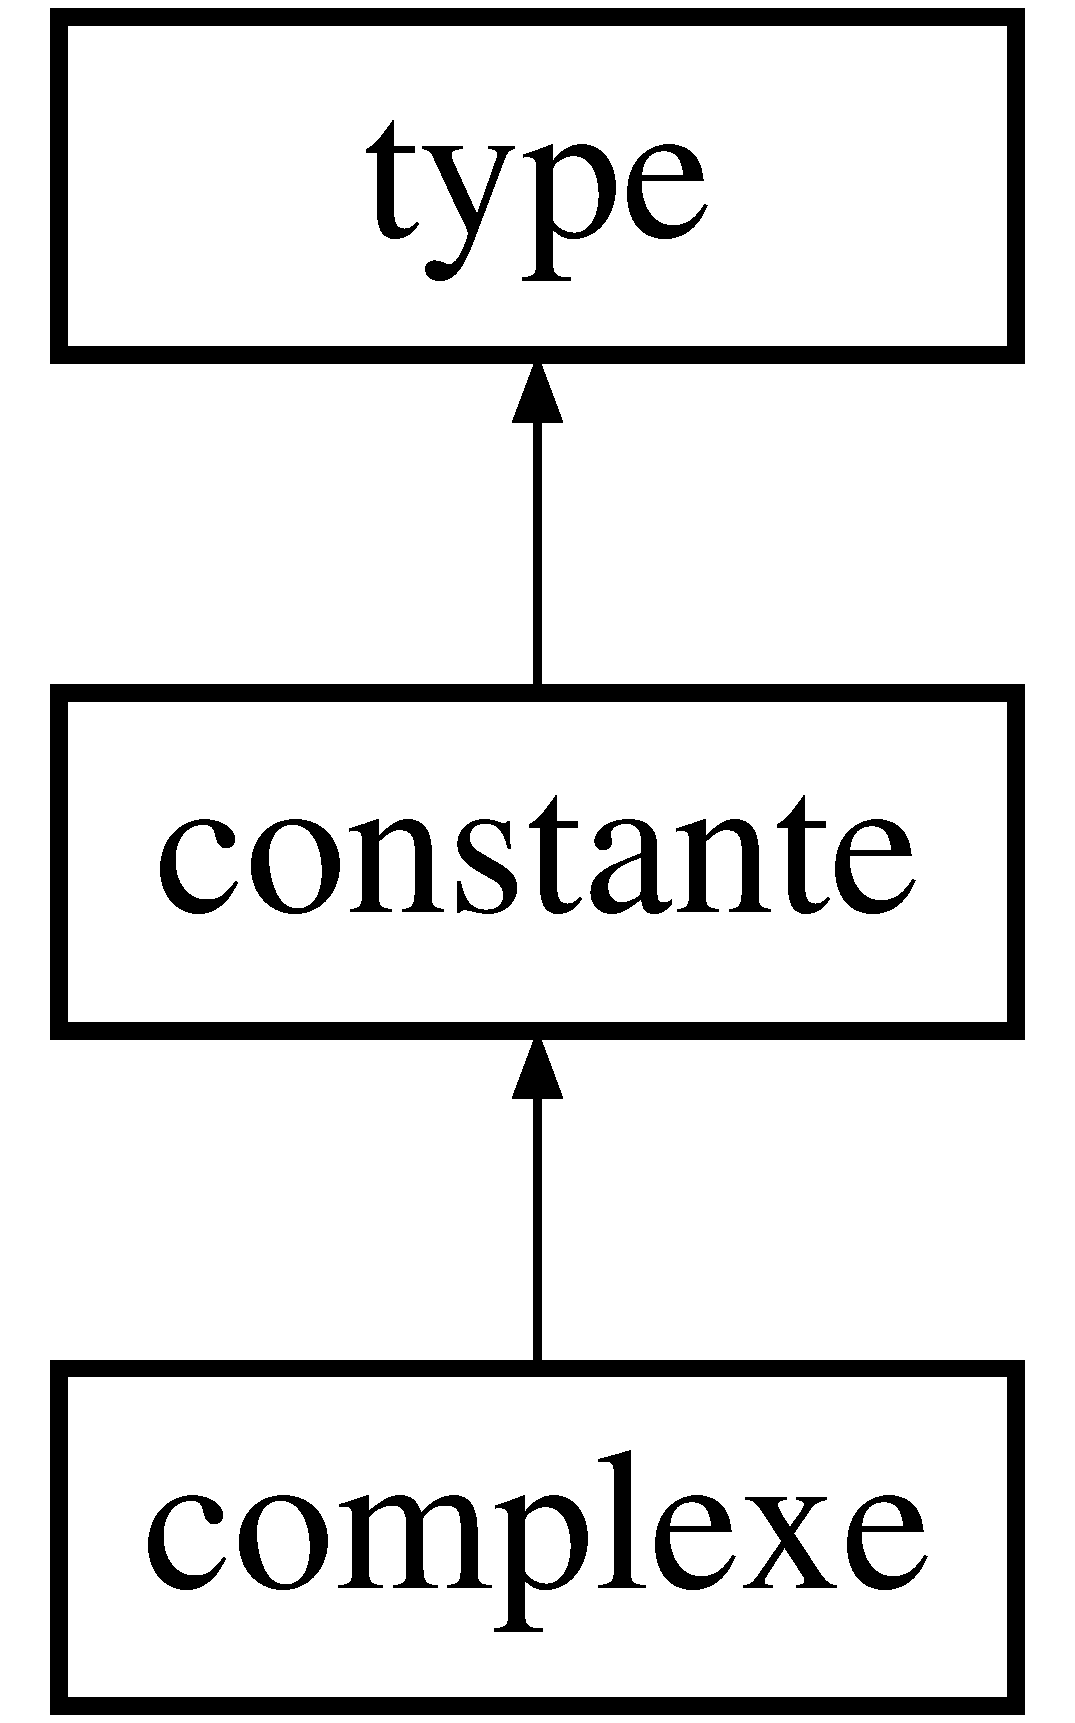
\includegraphics[height=3.000000cm]{classcomplexe}
\end{center}
\end{figure}
\subsection*{Public Member Functions}
\begin{DoxyCompactItemize}
\item 
\hyperlink{classcomplexe_adc78653349f4c9d9c649fcc3dd40ee41}{complexe} (\hyperlink{classnocomplex}{nocomplex} $\ast$\-\_\-re=0, \hyperlink{classnocomplex}{nocomplex} $\ast$\-\_\-im=0)
\begin{DoxyCompactList}\small\item\em Constructeur. \end{DoxyCompactList}\item 
\hypertarget{classcomplexe_a2f8b146111837f4b2f60e704ee6e0632}{\hyperlink{classtype}{type} $\ast$ {\bfseries conjugue} ()}\label{classcomplexe_a2f8b146111837f4b2f60e704ee6e0632}

\item 
\hyperlink{classcomplexe_ac69dfe1d10fc970cab943111831c5e59}{complexe} (const Q\-String \&s)
\begin{DoxyCompactList}\small\item\em Constructeur. \end{DoxyCompactList}\item 
\hyperlink{classtype}{type} $\ast$ \hyperlink{classcomplexe_a9f98da0548d8b73f1f10f248061d196b}{operator+} (\hyperlink{classtype}{type} \&t)
\begin{DoxyCompactList}\small\item\em Operateur +. \end{DoxyCompactList}\item 
\hyperlink{classtype}{type} $\ast$ \hyperlink{classcomplexe_af2faf54f25b3e58699ecf1d0b6409603}{operator/} (\hyperlink{classtype}{type} \&t)
\begin{DoxyCompactList}\small\item\em Operateur /. \end{DoxyCompactList}\item 
\hyperlink{classtype}{type} $\ast$ \hyperlink{classcomplexe_a02371b6578996af8af11f260931259b4}{operator$\ast$} (\hyperlink{classtype}{type} \&t)
\begin{DoxyCompactList}\small\item\em Operateur $\ast$. \end{DoxyCompactList}\item 
\hyperlink{classtype}{type} $\ast$ \hyperlink{classcomplexe_ae74ae6a7236ccbdaf74e88e5464ffb43}{operator-\/} (\hyperlink{classtype}{type} \&t)
\begin{DoxyCompactList}\small\item\em Operateur -\/. \end{DoxyCompactList}\item 
\hyperlink{classtype}{type} $\ast$ \hyperlink{classcomplexe_a9e7f59cfa1dd74f77891d7bfd1c1c62b}{sign} ()
\begin{DoxyCompactList}\small\item\em sign Operateur unaire sign Methode virtuelle \end{DoxyCompactList}\item 
\hyperlink{classnocomplex}{nocomplex} $\ast$ \hyperlink{classcomplexe_aed1ac631e9354b052b89913a8bc18b1d}{get\-Re} ()
\begin{DoxyCompactList}\small\item\em get\-Re \end{DoxyCompactList}\item 
\hyperlink{classnocomplex}{nocomplex} $\ast$ \hyperlink{classcomplexe_a3a2b9bf78d9e6cdbf2c533c2392fef4c}{get\-Im} ()
\begin{DoxyCompactList}\small\item\em get\-Im \end{DoxyCompactList}\item 
Q\-String \hyperlink{classcomplexe_a5fc10d08facdcbd833d91d0c765c9c18}{to\-Q\-String} ()
\begin{DoxyCompactList}\small\item\em to\-Q\-String \end{DoxyCompactList}\end{DoxyCompactItemize}


\subsection{Detailed Description}
Classe representant un complexe. 

La classe gere la partie reelle et la partie imaginaire des complexes et permet les operations classiques. Derive de la classe constante 

\subsection{Constructor \& Destructor Documentation}
\hypertarget{classcomplexe_adc78653349f4c9d9c649fcc3dd40ee41}{\index{complexe@{complexe}!complexe@{complexe}}
\index{complexe@{complexe}!complexe@{complexe}}
\subsubsection[{complexe}]{\setlength{\rightskip}{0pt plus 5cm}complexe\-::complexe (
\begin{DoxyParamCaption}
\item[{{\bf nocomplex} $\ast$}]{\-\_\-re = {\ttfamily 0}, }
\item[{{\bf nocomplex} $\ast$}]{\-\_\-im = {\ttfamily 0}}
\end{DoxyParamCaption}
)\hspace{0.3cm}{\ttfamily [inline]}}}\label{classcomplexe_adc78653349f4c9d9c649fcc3dd40ee41}


Constructeur. 

Constructeur a partir de pointeurs sur \char`\"{}nocomplex\char`\"{} 
\begin{DoxyParams}{Parameters}
{\em \-\_\-re} & \-: partie relle, pointeur sur nocomplex,0 par defaut \-\_\-im \-: partie imagianaire, pointeur sur nocomplex,0 par defaut \\
\hline
\end{DoxyParams}
\hypertarget{classcomplexe_ac69dfe1d10fc970cab943111831c5e59}{\index{complexe@{complexe}!complexe@{complexe}}
\index{complexe@{complexe}!complexe@{complexe}}
\subsubsection[{complexe}]{\setlength{\rightskip}{0pt plus 5cm}complexe\-::complexe (
\begin{DoxyParamCaption}
\item[{const Q\-String \&}]{s}
\end{DoxyParamCaption}
)\hspace{0.3cm}{\ttfamily [inline]}}}\label{classcomplexe_ac69dfe1d10fc970cab943111831c5e59}


Constructeur. 

Constructeur a partir de Qstring. Parse la chaine pour construire un complexe 
\begin{DoxyParams}{Parameters}
{\em s} & \-: Qstring, par reference \\
\hline
\end{DoxyParams}


\subsection{Member Function Documentation}
\hypertarget{classcomplexe_a3a2b9bf78d9e6cdbf2c533c2392fef4c}{\index{complexe@{complexe}!get\-Im@{get\-Im}}
\index{get\-Im@{get\-Im}!complexe@{complexe}}
\subsubsection[{get\-Im}]{\setlength{\rightskip}{0pt plus 5cm}{\bf nocomplex}$\ast$ complexe\-::get\-Im (
\begin{DoxyParamCaption}
{}
\end{DoxyParamCaption}
)\hspace{0.3cm}{\ttfamily [inline]}}}\label{classcomplexe_a3a2b9bf78d9e6cdbf2c533c2392fef4c}


get\-Im 

Accesseur de la partie reelle \begin{DoxyReturn}{Returns}
Pointeur sur nocomplex, partie imaginaire de l'objet appelant 
\end{DoxyReturn}
\hypertarget{classcomplexe_aed1ac631e9354b052b89913a8bc18b1d}{\index{complexe@{complexe}!get\-Re@{get\-Re}}
\index{get\-Re@{get\-Re}!complexe@{complexe}}
\subsubsection[{get\-Re}]{\setlength{\rightskip}{0pt plus 5cm}{\bf nocomplex}$\ast$ complexe\-::get\-Re (
\begin{DoxyParamCaption}
{}
\end{DoxyParamCaption}
)\hspace{0.3cm}{\ttfamily [inline]}}}\label{classcomplexe_aed1ac631e9354b052b89913a8bc18b1d}


get\-Re 

Accesseur de la partie reelle \begin{DoxyReturn}{Returns}
Pointeur sur nocomplex, partie reelle de l'objet appelant 
\end{DoxyReturn}
\hypertarget{classcomplexe_a02371b6578996af8af11f260931259b4}{\index{complexe@{complexe}!operator$\ast$@{operator$\ast$}}
\index{operator$\ast$@{operator$\ast$}!complexe@{complexe}}
\subsubsection[{operator$\ast$}]{\setlength{\rightskip}{0pt plus 5cm}{\bf type} $\ast$ complexe\-::operator$\ast$ (
\begin{DoxyParamCaption}
\item[{{\bf type} \&}]{t}
\end{DoxyParamCaption}
)\hspace{0.3cm}{\ttfamily [virtual]}}}\label{classcomplexe_a02371b6578996af8af11f260931259b4}


Operateur $\ast$. 

Implementation de l'operateur binaire $\ast$ (methode virtuelle dans la classe mere) 
\begin{DoxyParams}{Parameters}
{\em t} & \-: Pointeur sur un type \\
\hline
\end{DoxyParams}
\begin{DoxyReturn}{Returns}
Pointeur sur type, resultat de l'operation 
\end{DoxyReturn}


Implements \hyperlink{classtype_a9e275d2b8465d6085515f58aaf631ea7}{type}.

\hypertarget{classcomplexe_a9f98da0548d8b73f1f10f248061d196b}{\index{complexe@{complexe}!operator+@{operator+}}
\index{operator+@{operator+}!complexe@{complexe}}
\subsubsection[{operator+}]{\setlength{\rightskip}{0pt plus 5cm}{\bf type} $\ast$ complexe\-::operator+ (
\begin{DoxyParamCaption}
\item[{{\bf type} \&}]{t}
\end{DoxyParamCaption}
)\hspace{0.3cm}{\ttfamily [virtual]}}}\label{classcomplexe_a9f98da0548d8b73f1f10f248061d196b}


Operateur +. 

Implementation de l'operateur binaire + (methode virtuelle dans la classe mere) 
\begin{DoxyParams}{Parameters}
{\em t} & \-: Pointeur sur un type \\
\hline
\end{DoxyParams}
\begin{DoxyReturn}{Returns}
Pointeur sur type, resultat de l'operation 
\end{DoxyReturn}


Implements \hyperlink{classtype_aae435de533d21af297434702fd71d04d}{type}.

\hypertarget{classcomplexe_ae74ae6a7236ccbdaf74e88e5464ffb43}{\index{complexe@{complexe}!operator-\/@{operator-\/}}
\index{operator-\/@{operator-\/}!complexe@{complexe}}
\subsubsection[{operator-\/}]{\setlength{\rightskip}{0pt plus 5cm}{\bf type} $\ast$ complexe\-::operator-\/ (
\begin{DoxyParamCaption}
\item[{{\bf type} \&}]{t}
\end{DoxyParamCaption}
)\hspace{0.3cm}{\ttfamily [virtual]}}}\label{classcomplexe_ae74ae6a7236ccbdaf74e88e5464ffb43}


Operateur -\/. 

Implementation de l'operateur binaire -\/ (methode virtuelle dans la classe mere) 
\begin{DoxyParams}{Parameters}
{\em t} & \-: Pointeur sur un type \\
\hline
\end{DoxyParams}
\begin{DoxyReturn}{Returns}
Pointeur sur type, resultat de l'operation 
\end{DoxyReturn}


Implements \hyperlink{classtype_a4d440ee89d624d7314786d8d18751588}{type}.

\hypertarget{classcomplexe_af2faf54f25b3e58699ecf1d0b6409603}{\index{complexe@{complexe}!operator/@{operator/}}
\index{operator/@{operator/}!complexe@{complexe}}
\subsubsection[{operator/}]{\setlength{\rightskip}{0pt plus 5cm}{\bf type} $\ast$ complexe\-::operator/ (
\begin{DoxyParamCaption}
\item[{{\bf type} \&}]{t}
\end{DoxyParamCaption}
)\hspace{0.3cm}{\ttfamily [virtual]}}}\label{classcomplexe_af2faf54f25b3e58699ecf1d0b6409603}


Operateur /. 

Implementation de l'operateur binaire / (methode virtuelle dans la classe mere) 
\begin{DoxyParams}{Parameters}
{\em t} & \-: Pointeur sur un type \\
\hline
\end{DoxyParams}
\begin{DoxyReturn}{Returns}
Pointeur sur type, resultat de l'operation 
\end{DoxyReturn}


Implements \hyperlink{classtype_a0fad8179d45b9bbde90b48e1950ce639}{type}.

\hypertarget{classcomplexe_a9e7f59cfa1dd74f77891d7bfd1c1c62b}{\index{complexe@{complexe}!sign@{sign}}
\index{sign@{sign}!complexe@{complexe}}
\subsubsection[{sign}]{\setlength{\rightskip}{0pt plus 5cm}{\bf type} $\ast$ complexe\-::sign (
\begin{DoxyParamCaption}
{}
\end{DoxyParamCaption}
)\hspace{0.3cm}{\ttfamily [virtual]}}}\label{classcomplexe_a9e7f59cfa1dd74f77891d7bfd1c1c62b}


sign Operateur unaire sign Methode virtuelle 

\begin{DoxyReturn}{Returns}
Pointeur sur type, resultat de l'operation 
\end{DoxyReturn}


Reimplemented from \hyperlink{classtype_a3ec9f31aec3ddc52efe2adff634a671a}{type}.

\hypertarget{classcomplexe_a5fc10d08facdcbd833d91d0c765c9c18}{\index{complexe@{complexe}!to\-Q\-String@{to\-Q\-String}}
\index{to\-Q\-String@{to\-Q\-String}!complexe@{complexe}}
\subsubsection[{to\-Q\-String}]{\setlength{\rightskip}{0pt plus 5cm}Q\-String complexe\-::to\-Q\-String (
\begin{DoxyParamCaption}
{}
\end{DoxyParamCaption}
)\hspace{0.3cm}{\ttfamily [virtual]}}}\label{classcomplexe_a5fc10d08facdcbd833d91d0c765c9c18}


to\-Q\-String 

Transforme l'objet Qstring. Permet ensuite l'affichage dans des widget \begin{DoxyReturn}{Returns}
Qstring \-: chaine resultat 
\end{DoxyReturn}


Implements \hyperlink{classtype_ab61f01d56f3896cc99788a1a18c4b0c2}{type}.



The documentation for this class was generated from the following files\-:\begin{DoxyCompactItemize}
\item 
Code/projet\-\_\-lo21/\hyperlink{complexe_8h}{complexe.\-h}\item 
Code/projet\-\_\-lo21/complexe.\-cpp\end{DoxyCompactItemize}

\hypertarget{classconstante}{\section{constante Class Reference}
\label{classconstante}\index{constante@{constante}}
}


Classe representant une constante.  




{\ttfamily \#include $<$constante.\-h$>$}

Inheritance diagram for constante\-:\begin{figure}[H]
\begin{center}
\leavevmode
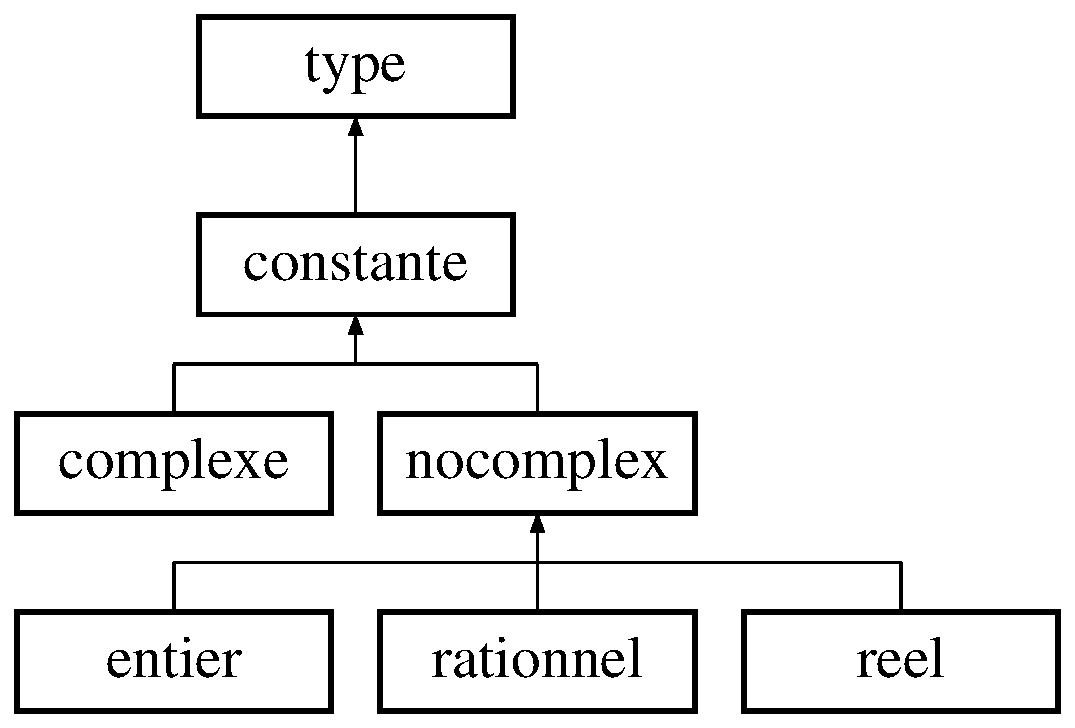
\includegraphics[height=4.000000cm]{classconstante}
\end{center}
\end{figure}
\subsection*{Additional Inherited Members}


\subsection{Detailed Description}
Classe representant une constante. 

La classe derive de type. Permet d'obtenir une arborescence classe coherente 

The documentation for this class was generated from the following file\-:\begin{DoxyCompactItemize}
\item 
Code/projet\-\_\-lo21/constante.\-h\end{DoxyCompactItemize}

\hypertarget{class_dom}{\section{Dom Class Reference}
\label{class_dom}\index{Dom@{Dom}}
}


{\ttfamily \#include $<$dom.\-h$>$}

\subsection*{Public Member Functions}
\begin{DoxyCompactItemize}
\item 
\hyperlink{class_dom_a76622d9817909851b9e7ba8a9b3d2614}{Dom} (\hyperlink{class_pile}{Pile} \&p)
\item 
\hyperlink{class_dom_a5f1552721661519991b402047c661881}{$\sim$\-Dom} ()
\item 
void \hyperlink{class_dom_ae871a6f3df66dd25a60dc6473849afa4}{demande\-\_\-ajout} (Q\-String, Q\-String)
\item 
void \hyperlink{class_dom_a6ee5457023816c5ed79606e3e9abc17e}{lire} ()
\item 
void \hyperlink{class_dom_a502b476ad2ff4b00c5139694f29994af}{newfic} ()
\end{DoxyCompactItemize}


\subsection{Constructor \& Destructor Documentation}
\hypertarget{class_dom_a76622d9817909851b9e7ba8a9b3d2614}{\index{Dom@{Dom}!Dom@{Dom}}
\index{Dom@{Dom}!Dom@{Dom}}
\subsubsection[{Dom}]{\setlength{\rightskip}{0pt plus 5cm}Dom\-::\-Dom (
\begin{DoxyParamCaption}
\item[{{\bf Pile} \&}]{p}
\end{DoxyParamCaption}
)}}\label{class_dom_a76622d9817909851b9e7ba8a9b3d2614}
\hypertarget{class_dom_a5f1552721661519991b402047c661881}{\index{Dom@{Dom}!$\sim$\-Dom@{$\sim$\-Dom}}
\index{$\sim$\-Dom@{$\sim$\-Dom}!Dom@{Dom}}
\subsubsection[{$\sim$\-Dom}]{\setlength{\rightskip}{0pt plus 5cm}Dom\-::$\sim$\-Dom (
\begin{DoxyParamCaption}
{}
\end{DoxyParamCaption}
)}}\label{class_dom_a5f1552721661519991b402047c661881}


\subsection{Member Function Documentation}
\hypertarget{class_dom_ae871a6f3df66dd25a60dc6473849afa4}{\index{Dom@{Dom}!demande\-\_\-ajout@{demande\-\_\-ajout}}
\index{demande\-\_\-ajout@{demande\-\_\-ajout}!Dom@{Dom}}
\subsubsection[{demande\-\_\-ajout}]{\setlength{\rightskip}{0pt plus 5cm}void Dom\-::demande\-\_\-ajout (
\begin{DoxyParamCaption}
\item[{Q\-String}]{n, }
\item[{Q\-String}]{t}
\end{DoxyParamCaption}
)}}\label{class_dom_ae871a6f3df66dd25a60dc6473849afa4}
\hypertarget{class_dom_a6ee5457023816c5ed79606e3e9abc17e}{\index{Dom@{Dom}!lire@{lire}}
\index{lire@{lire}!Dom@{Dom}}
\subsubsection[{lire}]{\setlength{\rightskip}{0pt plus 5cm}void Dom\-::lire (
\begin{DoxyParamCaption}
{}
\end{DoxyParamCaption}
)}}\label{class_dom_a6ee5457023816c5ed79606e3e9abc17e}
\hypertarget{class_dom_a502b476ad2ff4b00c5139694f29994af}{\index{Dom@{Dom}!newfic@{newfic}}
\index{newfic@{newfic}!Dom@{Dom}}
\subsubsection[{newfic}]{\setlength{\rightskip}{0pt plus 5cm}void Dom\-::newfic (
\begin{DoxyParamCaption}
{}
\end{DoxyParamCaption}
)}}\label{class_dom_a502b476ad2ff4b00c5139694f29994af}


The documentation for this class was generated from the following files\-:\begin{DoxyCompactItemize}
\item 
Code/projet\-\_\-lo21/\hyperlink{dom_8h}{dom.\-h}\item 
Code/projet\-\_\-lo21/\hyperlink{dom_8cpp}{dom.\-cpp}\end{DoxyCompactItemize}

\hypertarget{classentier}{\section{entier Class Reference}
\label{classentier}\index{entier@{entier}}
}


Classe representant une constante.  




{\ttfamily \#include $<$entier.\-h$>$}

Inheritance diagram for entier\-:\begin{figure}[H]
\begin{center}
\leavevmode
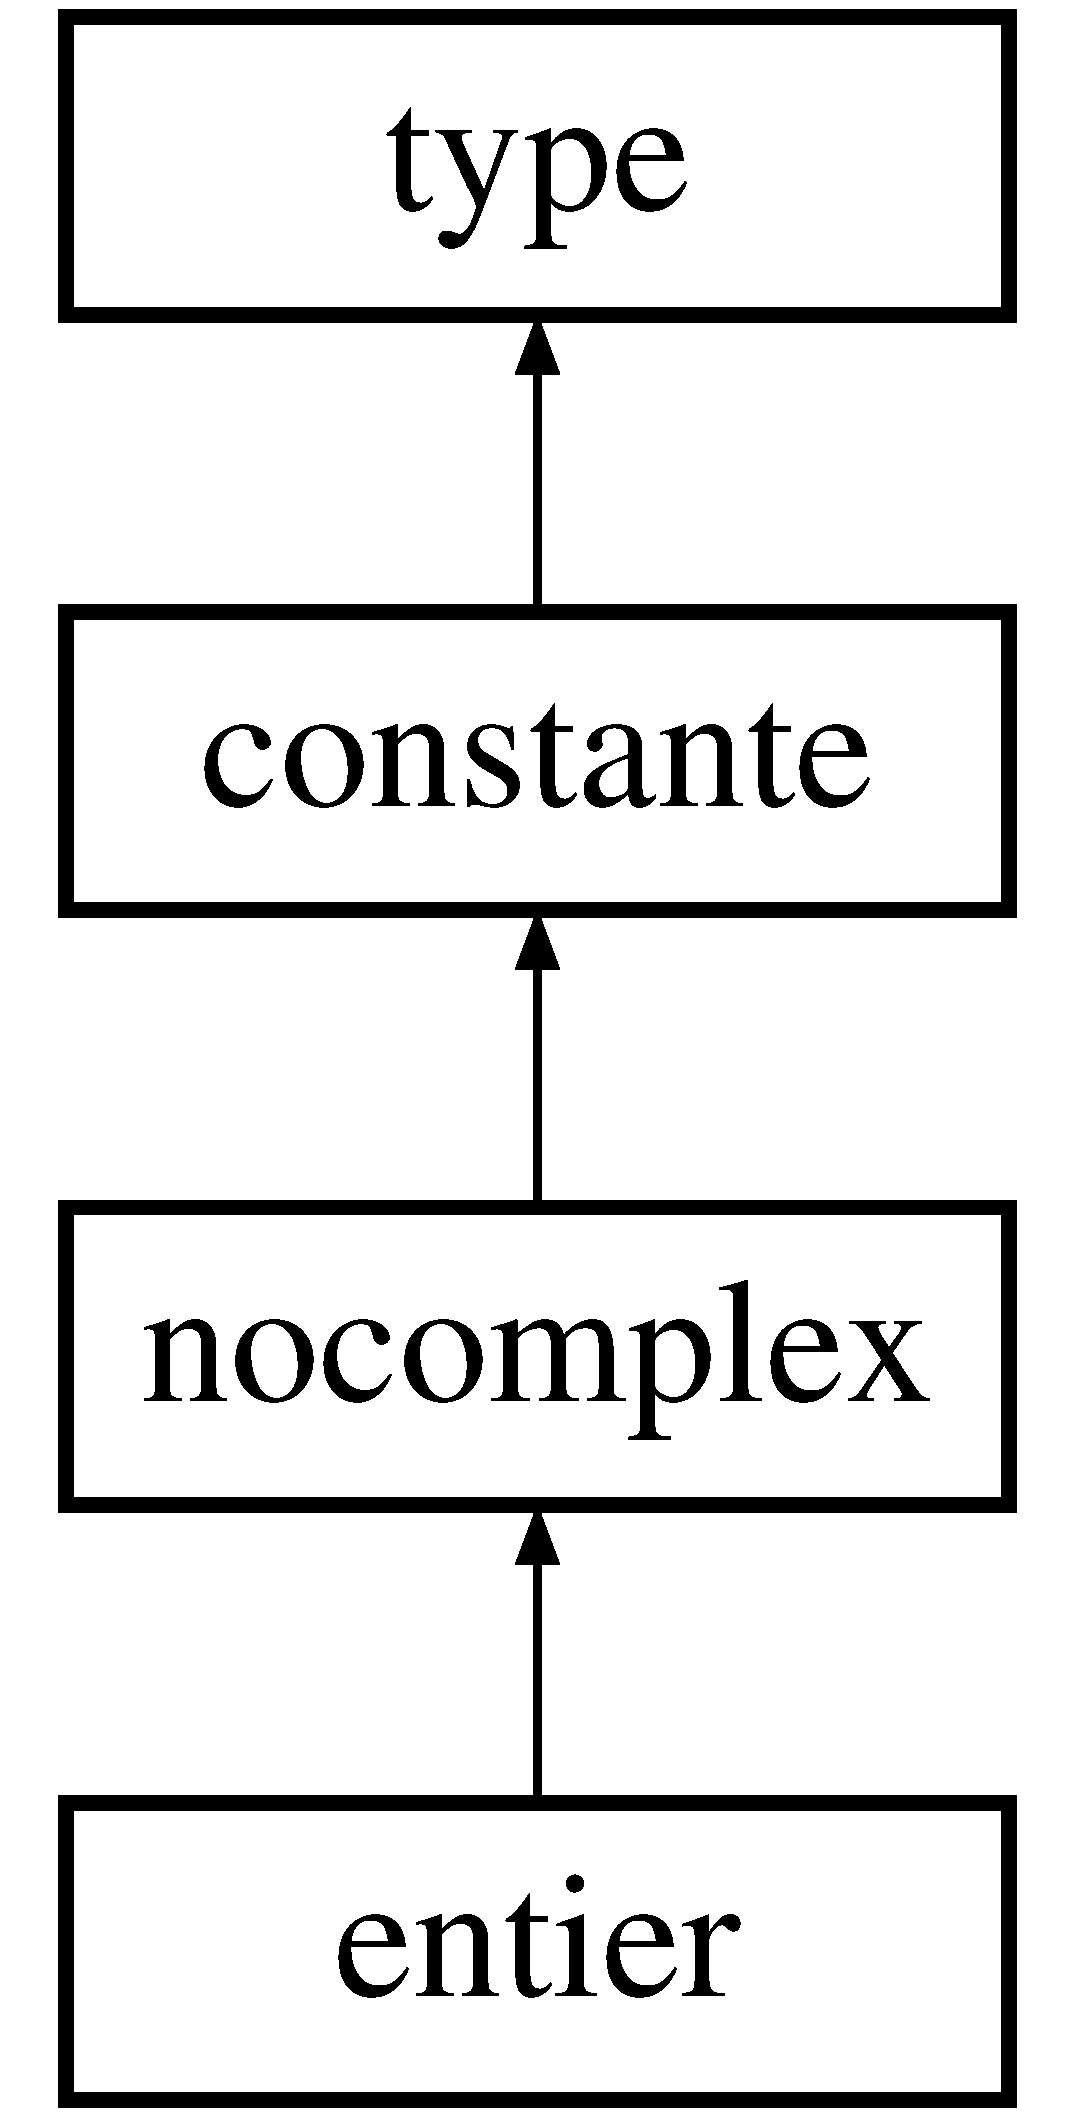
\includegraphics[height=4.000000cm]{classentier}
\end{center}
\end{figure}
\subsection*{Public Member Functions}
\begin{DoxyCompactItemize}
\item 
\hyperlink{classentier_ad1b9eb5e221dfc5006527edda8c19f8a}{entier} (int val=0)
\begin{DoxyCompactList}\small\item\em Constructeur. \end{DoxyCompactList}\item 
\hyperlink{classentier_aeee175a8cb61246f25e1ddafefebe820}{entier} (const Q\-String \&s)
\begin{DoxyCompactList}\small\item\em Constructeur. \end{DoxyCompactList}\item 
int \hyperlink{classentier_a738d3684bb420ffb5bbee2187845af85}{get\-Data} ()
\begin{DoxyCompactList}\small\item\em get\-Data \end{DoxyCompactList}\item 
\hyperlink{classtype}{type} $\ast$ \hyperlink{classentier_a531e654172d6e2fe225fad108dbb84a7}{operator+} (\hyperlink{classtype}{type} \&t)
\begin{DoxyCompactList}\small\item\em Operateur +. \end{DoxyCompactList}\item 
\hyperlink{classtype}{type} $\ast$ \hyperlink{classentier_a3bfd34b6998c5c09df0dbbadead47867}{operator/} (\hyperlink{classtype}{type} \&t)
\begin{DoxyCompactList}\small\item\em Operateur /. \end{DoxyCompactList}\item 
\hyperlink{classtype}{type} $\ast$ \hyperlink{classentier_a7314a5aad4a2c997eaea01e3aa42092a}{operator$\ast$} (\hyperlink{classtype}{type} \&t)
\begin{DoxyCompactList}\small\item\em Operateur $\ast$. \end{DoxyCompactList}\item 
\hyperlink{classtype}{type} $\ast$ \hyperlink{classentier_ac0acf2b6156ef6f5f2e034c0425e1114}{operator-\/} (\hyperlink{classtype}{type} \&t)
\begin{DoxyCompactList}\small\item\em Operateur -\/. \end{DoxyCompactList}\item 
\hyperlink{classtype}{type} $\ast$ \hyperlink{classentier_a5dd86ffdc48bf745871ac2f65199d2ce}{sinus} (bool degre=false)
\begin{DoxyCompactList}\small\item\em Sinus. \end{DoxyCompactList}\item 
\hyperlink{classtype}{type} $\ast$ \hyperlink{classentier_adc71e10e6ea385f7c1aa1de06e2d1b4c}{pow} (\hyperlink{classtype}{type} \&t)
\begin{DoxyCompactList}\small\item\em Pow. \end{DoxyCompactList}\item 
\hyperlink{classtype}{type} $\ast$ \hyperlink{classentier_a4e5c25c0ed52135136bb75563a9337e7}{mod} (\hyperlink{classtype}{type} \&t)
\begin{DoxyCompactList}\small\item\em mod \end{DoxyCompactList}\item 
\hyperlink{classtype}{type} $\ast$ \hyperlink{classentier_a4a25b08f29eba0a531bebadeaf77ee04}{sign} ()
\begin{DoxyCompactList}\small\item\em sign \end{DoxyCompactList}\item 
\hyperlink{classtype}{type} $\ast$ \hyperlink{classentier_a1313e6cfa480cab69942f9b97418e491}{cosinus} (bool degre=false)
\begin{DoxyCompactList}\small\item\em Cosinus. \end{DoxyCompactList}\item 
\hyperlink{classtype}{type} $\ast$ \hyperlink{classentier_a600a48ecf8280f0ab465ab3f3c253662}{tangente} (bool degre=false)
\begin{DoxyCompactList}\small\item\em Tangente. \end{DoxyCompactList}\item 
\hyperlink{classtype}{type} $\ast$ \hyperlink{classentier_abfb8840f088a4771520fd48a78c01434}{sinush} (bool degre=false)
\begin{DoxyCompactList}\small\item\em Sinush. \end{DoxyCompactList}\item 
\hyperlink{classtype}{type} $\ast$ \hyperlink{classentier_af111db8d7c89d47f20c59e3bd0ef1dfd}{cosinush} (bool degre=false)
\begin{DoxyCompactList}\small\item\em Cosinush. \end{DoxyCompactList}\item 
\hyperlink{classtype}{type} $\ast$ \hyperlink{classentier_abd47ffc368af385550ed2db6ce289ded}{tangenteh} (bool degre=false)
\begin{DoxyCompactList}\small\item\em Tangenteh. \end{DoxyCompactList}\item 
\hyperlink{classtype}{type} $\ast$ \hyperlink{classentier_aef2c65b9f379c5ea7857fcaabca30dba}{ln} ()
\begin{DoxyCompactList}\small\item\em Ln. \end{DoxyCompactList}\item 
\hyperlink{classtype}{type} $\ast$ \hyperlink{classentier_aeca6cf72ceaa32cfc7b52f00d962d3cc}{log} ()
\begin{DoxyCompactList}\small\item\em Log. \end{DoxyCompactList}\item 
\hyperlink{classtype}{type} $\ast$ \hyperlink{classentier_abaa5775172cf9c417ccdb174304056b3}{inv} ()
\begin{DoxyCompactList}\small\item\em Inv. \end{DoxyCompactList}\item 
\hyperlink{classtype}{type} $\ast$ \hyperlink{classentier_a9058b76c3fae96fb3a9ade24e6c33926}{sqrt} ()
\begin{DoxyCompactList}\small\item\em Sqrt. \end{DoxyCompactList}\item 
\hyperlink{classtype}{type} $\ast$ \hyperlink{classentier_a33b0b2b13a0fdc767a809df33b934dd6}{sqr} ()
\begin{DoxyCompactList}\small\item\em Sqr. \end{DoxyCompactList}\item 
\hyperlink{classtype}{type} $\ast$ \hyperlink{classentier_a4c726d947d2f7464ec858f50054118e8}{cube} ()
\begin{DoxyCompactList}\small\item\em Cube. \end{DoxyCompactList}\item 
\hyperlink{classtype}{type} $\ast$ \hyperlink{classentier_a8a475a326fc2c4e1b2a03ec437270144}{fact} ()
\begin{DoxyCompactList}\small\item\em Fact. \end{DoxyCompactList}\item 
Q\-String \hyperlink{classentier_a47b7c0d899f24e9117e123165648686b}{to\-Q\-String} ()
\begin{DoxyCompactList}\small\item\em to\-Q\-String \end{DoxyCompactList}\end{DoxyCompactItemize}


\subsection{Detailed Description}
Classe representant une constante. 

La classe derive de nocomplex. Permet de representer un entier 

\subsection{Constructor \& Destructor Documentation}
\hypertarget{classentier_ad1b9eb5e221dfc5006527edda8c19f8a}{\index{entier@{entier}!entier@{entier}}
\index{entier@{entier}!entier@{entier}}
\subsubsection[{entier}]{\setlength{\rightskip}{0pt plus 5cm}entier\-::entier (
\begin{DoxyParamCaption}
\item[{int}]{val = {\ttfamily 0}}
\end{DoxyParamCaption}
)\hspace{0.3cm}{\ttfamily [inline]}}}\label{classentier_ad1b9eb5e221dfc5006527edda8c19f8a}


Constructeur. 

Constructeur a partir d'un entier 
\begin{DoxyParams}{Parameters}
{\em val} & \-: valeur de l'entier \\
\hline
\end{DoxyParams}
\hypertarget{classentier_aeee175a8cb61246f25e1ddafefebe820}{\index{entier@{entier}!entier@{entier}}
\index{entier@{entier}!entier@{entier}}
\subsubsection[{entier}]{\setlength{\rightskip}{0pt plus 5cm}entier\-::entier (
\begin{DoxyParamCaption}
\item[{const Q\-String \&}]{s}
\end{DoxyParamCaption}
)\hspace{0.3cm}{\ttfamily [inline]}}}\label{classentier_aeee175a8cb61246f25e1ddafefebe820}


Constructeur. 

Constructeur a partir d'une Qstring 
\begin{DoxyParams}{Parameters}
{\em s} & \-: chaine source \\
\hline
\end{DoxyParams}


\subsection{Member Function Documentation}
\hypertarget{classentier_a1313e6cfa480cab69942f9b97418e491}{\index{entier@{entier}!cosinus@{cosinus}}
\index{cosinus@{cosinus}!entier@{entier}}
\subsubsection[{cosinus}]{\setlength{\rightskip}{0pt plus 5cm}{\bf type} $\ast$ entier\-::cosinus (
\begin{DoxyParamCaption}
\item[{bool}]{degre = {\ttfamily false}}
\end{DoxyParamCaption}
)\hspace{0.3cm}{\ttfamily [virtual]}}}\label{classentier_a1313e6cfa480cab69942f9b97418e491}


Cosinus. 

Implementation de l'operateur unaire cosinus (methode virtuelle dans la classe mere) \begin{DoxyReturn}{Returns}
Pointeur sur type, resultat de l'operation 
\end{DoxyReturn}


Implements \hyperlink{classnocomplex_a2c3aa4791fe0c123079b0332a5978939}{nocomplex}.

\hypertarget{classentier_af111db8d7c89d47f20c59e3bd0ef1dfd}{\index{entier@{entier}!cosinush@{cosinush}}
\index{cosinush@{cosinush}!entier@{entier}}
\subsubsection[{cosinush}]{\setlength{\rightskip}{0pt plus 5cm}{\bf type} $\ast$ entier\-::cosinush (
\begin{DoxyParamCaption}
\item[{bool}]{degre = {\ttfamily false}}
\end{DoxyParamCaption}
)\hspace{0.3cm}{\ttfamily [virtual]}}}\label{classentier_af111db8d7c89d47f20c59e3bd0ef1dfd}


Cosinush. 

Implementation de l'operateur unaire cosinush (methode virtuelle dans la classe mere) 
\begin{DoxyParams}{Parameters}
{\em degre} & \-: booleen, vrai si utilisation des degre, faux si utilisation des radians \\
\hline
\end{DoxyParams}
\begin{DoxyReturn}{Returns}
Pointeur sur type, resultat de l'operation 
\end{DoxyReturn}


Implements \hyperlink{classnocomplex_ae92516f1c7c78298a11e8e34355b9f81}{nocomplex}.

\hypertarget{classentier_a4c726d947d2f7464ec858f50054118e8}{\index{entier@{entier}!cube@{cube}}
\index{cube@{cube}!entier@{entier}}
\subsubsection[{cube}]{\setlength{\rightskip}{0pt plus 5cm}{\bf type} $\ast$ entier\-::cube (
\begin{DoxyParamCaption}
{}
\end{DoxyParamCaption}
)\hspace{0.3cm}{\ttfamily [virtual]}}}\label{classentier_a4c726d947d2f7464ec858f50054118e8}


Cube. 

Implementation de l'operateur unaire Cube (methode virtuelle dans la classe mere) \begin{DoxyReturn}{Returns}
Pointeur sur type, resultat de l'operation 
\end{DoxyReturn}


Implements \hyperlink{classnocomplex_ad84e4a7a269024da4551a8e99078e41d}{nocomplex}.

\hypertarget{classentier_a8a475a326fc2c4e1b2a03ec437270144}{\index{entier@{entier}!fact@{fact}}
\index{fact@{fact}!entier@{entier}}
\subsubsection[{fact}]{\setlength{\rightskip}{0pt plus 5cm}{\bf type} $\ast$ entier\-::fact (
\begin{DoxyParamCaption}
{}
\end{DoxyParamCaption}
)\hspace{0.3cm}{\ttfamily [virtual]}}}\label{classentier_a8a475a326fc2c4e1b2a03ec437270144}


Fact. 

Implementation de l'operateur unaire fact (methode virtuelle dans la classe mere) \begin{DoxyReturn}{Returns}
Pointeur sur type, resultat de l'operation 
\end{DoxyReturn}


Reimplemented from \hyperlink{classtype_adfeadf5e6478f3687bcaba9cf9aaf8d9}{type}.

\hypertarget{classentier_a738d3684bb420ffb5bbee2187845af85}{\index{entier@{entier}!get\-Data@{get\-Data}}
\index{get\-Data@{get\-Data}!entier@{entier}}
\subsubsection[{get\-Data}]{\setlength{\rightskip}{0pt plus 5cm}int entier\-::get\-Data (
\begin{DoxyParamCaption}
{}
\end{DoxyParamCaption}
)\hspace{0.3cm}{\ttfamily [inline]}}}\label{classentier_a738d3684bb420ffb5bbee2187845af85}


get\-Data 

Accesseur de la donnee membre data \begin{DoxyReturn}{Returns}
entier 
\end{DoxyReturn}
\hypertarget{classentier_abaa5775172cf9c417ccdb174304056b3}{\index{entier@{entier}!inv@{inv}}
\index{inv@{inv}!entier@{entier}}
\subsubsection[{inv}]{\setlength{\rightskip}{0pt plus 5cm}{\bf type} $\ast$ entier\-::inv (
\begin{DoxyParamCaption}
{}
\end{DoxyParamCaption}
)\hspace{0.3cm}{\ttfamily [virtual]}}}\label{classentier_abaa5775172cf9c417ccdb174304056b3}


Inv. 

Implementation de l'operateur unaire inv (methode virtuelle dans la classe mere) \begin{DoxyReturn}{Returns}
Pointeur sur type, resultat de l'operation 
\end{DoxyReturn}


Implements \hyperlink{classnocomplex_a9e0f97f51c50b11022c6d0b409c26ecf}{nocomplex}.

\hypertarget{classentier_aef2c65b9f379c5ea7857fcaabca30dba}{\index{entier@{entier}!ln@{ln}}
\index{ln@{ln}!entier@{entier}}
\subsubsection[{ln}]{\setlength{\rightskip}{0pt plus 5cm}{\bf type} $\ast$ entier\-::ln (
\begin{DoxyParamCaption}
{}
\end{DoxyParamCaption}
)\hspace{0.3cm}{\ttfamily [virtual]}}}\label{classentier_aef2c65b9f379c5ea7857fcaabca30dba}


Ln. 

Implementation de l'operateur unaire ln (methode virtuelle dans la classe mere) \begin{DoxyReturn}{Returns}
Pointeur sur type, resultat de l'operation 
\end{DoxyReturn}


Implements \hyperlink{classnocomplex_ab3e91b96595fef9d53a5cfb93291c8f0}{nocomplex}.

\hypertarget{classentier_aeca6cf72ceaa32cfc7b52f00d962d3cc}{\index{entier@{entier}!log@{log}}
\index{log@{log}!entier@{entier}}
\subsubsection[{log}]{\setlength{\rightskip}{0pt plus 5cm}{\bf type} $\ast$ entier\-::log (
\begin{DoxyParamCaption}
{}
\end{DoxyParamCaption}
)\hspace{0.3cm}{\ttfamily [virtual]}}}\label{classentier_aeca6cf72ceaa32cfc7b52f00d962d3cc}


Log. 

Implementation de l'operateur unaire log (methode virtuelle dans la classe mere) \begin{DoxyReturn}{Returns}
Pointeur sur type, resultat de l'operation 
\end{DoxyReturn}


Implements \hyperlink{classnocomplex_a0f7a5802123786d1461271d5c05158ca}{nocomplex}.

\hypertarget{classentier_a4e5c25c0ed52135136bb75563a9337e7}{\index{entier@{entier}!mod@{mod}}
\index{mod@{mod}!entier@{entier}}
\subsubsection[{mod}]{\setlength{\rightskip}{0pt plus 5cm}{\bf type} $\ast$ entier\-::mod (
\begin{DoxyParamCaption}
\item[{{\bf type} \&}]{t}
\end{DoxyParamCaption}
)\hspace{0.3cm}{\ttfamily [virtual]}}}\label{classentier_a4e5c25c0ed52135136bb75563a9337e7}


mod 

Implementation de l'operateur binaire modulo (methode virtuelle dans la classe mere) 
\begin{DoxyParams}{Parameters}
{\em t} & \-: Pointeur sur un type \\
\hline
\end{DoxyParams}
\begin{DoxyReturn}{Returns}
Pointeur sur type, resultat de l'operation 
\end{DoxyReturn}


Reimplemented from \hyperlink{classtype_aed752df353b43b17d3f993d4b02f216b}{type}.

\hypertarget{classentier_a7314a5aad4a2c997eaea01e3aa42092a}{\index{entier@{entier}!operator$\ast$@{operator$\ast$}}
\index{operator$\ast$@{operator$\ast$}!entier@{entier}}
\subsubsection[{operator$\ast$}]{\setlength{\rightskip}{0pt plus 5cm}{\bf type} $\ast$ entier\-::operator$\ast$ (
\begin{DoxyParamCaption}
\item[{{\bf type} \&}]{t}
\end{DoxyParamCaption}
)\hspace{0.3cm}{\ttfamily [virtual]}}}\label{classentier_a7314a5aad4a2c997eaea01e3aa42092a}


Operateur $\ast$. 

Implementation de l'operateur binaire $\ast$ (methode virtuelle dans la classe mere) 
\begin{DoxyParams}{Parameters}
{\em t} & \-: Pointeur sur un type \\
\hline
\end{DoxyParams}
\begin{DoxyReturn}{Returns}
Pointeur sur type, resultat de l'operation 
\end{DoxyReturn}


Implements \hyperlink{classnocomplex_ac84954cbe0bd9c77eab88c0b97b34c2b}{nocomplex}.

\hypertarget{classentier_a531e654172d6e2fe225fad108dbb84a7}{\index{entier@{entier}!operator+@{operator+}}
\index{operator+@{operator+}!entier@{entier}}
\subsubsection[{operator+}]{\setlength{\rightskip}{0pt plus 5cm}{\bf type} $\ast$ entier\-::operator+ (
\begin{DoxyParamCaption}
\item[{{\bf type} \&}]{t}
\end{DoxyParamCaption}
)\hspace{0.3cm}{\ttfamily [virtual]}}}\label{classentier_a531e654172d6e2fe225fad108dbb84a7}


Operateur +. 

Implementation de l'operateur binaire + (methode virtuelle dans la classe mere) 
\begin{DoxyParams}{Parameters}
{\em t} & \-: Pointeur sur un type \\
\hline
\end{DoxyParams}
\begin{DoxyReturn}{Returns}
Pointeur sur type, resultat de l'operation 
\end{DoxyReturn}


Implements \hyperlink{classnocomplex_af3d04b00f4f82d3a35cad0ca023093f4}{nocomplex}.

\hypertarget{classentier_ac0acf2b6156ef6f5f2e034c0425e1114}{\index{entier@{entier}!operator-\/@{operator-\/}}
\index{operator-\/@{operator-\/}!entier@{entier}}
\subsubsection[{operator-\/}]{\setlength{\rightskip}{0pt plus 5cm}{\bf type} $\ast$ entier\-::operator-\/ (
\begin{DoxyParamCaption}
\item[{{\bf type} \&}]{t}
\end{DoxyParamCaption}
)\hspace{0.3cm}{\ttfamily [virtual]}}}\label{classentier_ac0acf2b6156ef6f5f2e034c0425e1114}


Operateur -\/. 

Implementation de l'operateur binaire -\/ (methode virtuelle dans la classe mere) 
\begin{DoxyParams}{Parameters}
{\em t} & \-: Pointeur sur un type \\
\hline
\end{DoxyParams}
\begin{DoxyReturn}{Returns}
Pointeur sur type, resultat de l'operation 
\end{DoxyReturn}


Implements \hyperlink{classnocomplex_a2005c3a0fcaa1f360561539931ffc578}{nocomplex}.

\hypertarget{classentier_a3bfd34b6998c5c09df0dbbadead47867}{\index{entier@{entier}!operator/@{operator/}}
\index{operator/@{operator/}!entier@{entier}}
\subsubsection[{operator/}]{\setlength{\rightskip}{0pt plus 5cm}{\bf type} $\ast$ entier\-::operator/ (
\begin{DoxyParamCaption}
\item[{{\bf type} \&}]{t}
\end{DoxyParamCaption}
)\hspace{0.3cm}{\ttfamily [virtual]}}}\label{classentier_a3bfd34b6998c5c09df0dbbadead47867}


Operateur /. 

Implementation de l'operateur binaire / (methode virtuelle dans la classe mere) 
\begin{DoxyParams}{Parameters}
{\em t} & \-: Pointeur sur un type \\
\hline
\end{DoxyParams}
\begin{DoxyReturn}{Returns}
Pointeur sur type, resultat de l'operation 
\end{DoxyReturn}


Implements \hyperlink{classnocomplex_a47942bdcc78cfc5d5e867c9f9836a465}{nocomplex}.

\hypertarget{classentier_adc71e10e6ea385f7c1aa1de06e2d1b4c}{\index{entier@{entier}!pow@{pow}}
\index{pow@{pow}!entier@{entier}}
\subsubsection[{pow}]{\setlength{\rightskip}{0pt plus 5cm}{\bf type} $\ast$ entier\-::pow (
\begin{DoxyParamCaption}
\item[{{\bf type} \&}]{t}
\end{DoxyParamCaption}
)\hspace{0.3cm}{\ttfamily [virtual]}}}\label{classentier_adc71e10e6ea385f7c1aa1de06e2d1b4c}


Pow. 

Implementation de l'operateur binaire pow (methode virtuelle dans la classe mere) 
\begin{DoxyParams}{Parameters}
{\em t} & \-: Pointeur sur un type \\
\hline
\end{DoxyParams}
\begin{DoxyReturn}{Returns}
Pointeur sur type, resultat de l'operation 
\end{DoxyReturn}


Implements \hyperlink{classnocomplex_a1ad1b692783c8449efb03cc0dc5d1f3c}{nocomplex}.

\hypertarget{classentier_a4a25b08f29eba0a531bebadeaf77ee04}{\index{entier@{entier}!sign@{sign}}
\index{sign@{sign}!entier@{entier}}
\subsubsection[{sign}]{\setlength{\rightskip}{0pt plus 5cm}{\bf type} $\ast$ entier\-::sign (
\begin{DoxyParamCaption}
{}
\end{DoxyParamCaption}
)\hspace{0.3cm}{\ttfamily [virtual]}}}\label{classentier_a4a25b08f29eba0a531bebadeaf77ee04}


sign 

Implementation de l'operateur unaire sign (methode virtuelle dans la classe mere) Inverse le signe de la constante \begin{DoxyReturn}{Returns}
Pointeur sur type, resultat de l'operation 
\end{DoxyReturn}


Implements \hyperlink{classnocomplex_acd1c0365d1a2ed160934320cff01cecd}{nocomplex}.

\hypertarget{classentier_a5dd86ffdc48bf745871ac2f65199d2ce}{\index{entier@{entier}!sinus@{sinus}}
\index{sinus@{sinus}!entier@{entier}}
\subsubsection[{sinus}]{\setlength{\rightskip}{0pt plus 5cm}{\bf type} $\ast$ entier\-::sinus (
\begin{DoxyParamCaption}
\item[{bool}]{degre = {\ttfamily false}}
\end{DoxyParamCaption}
)\hspace{0.3cm}{\ttfamily [virtual]}}}\label{classentier_a5dd86ffdc48bf745871ac2f65199d2ce}


Sinus. 

Implementation de l'operateur unaire sinus (methode virtuelle dans la classe mere) 
\begin{DoxyParams}{Parameters}
{\em degre} & \-: booleen, vrai si utilisation des degre, faux si utilisation des radians \\
\hline
\end{DoxyParams}
\begin{DoxyReturn}{Returns}
Pointeur sur type, resultat de l'operation 
\end{DoxyReturn}


Implements \hyperlink{classnocomplex_aea2ba416f34c37ad2cf751b6220d53b8}{nocomplex}.

\hypertarget{classentier_abfb8840f088a4771520fd48a78c01434}{\index{entier@{entier}!sinush@{sinush}}
\index{sinush@{sinush}!entier@{entier}}
\subsubsection[{sinush}]{\setlength{\rightskip}{0pt plus 5cm}{\bf type} $\ast$ entier\-::sinush (
\begin{DoxyParamCaption}
\item[{bool}]{degre = {\ttfamily false}}
\end{DoxyParamCaption}
)\hspace{0.3cm}{\ttfamily [virtual]}}}\label{classentier_abfb8840f088a4771520fd48a78c01434}


Sinush. 

Implementation de l'operateur unaire sinush (methode virtuelle dans la classe mere) 
\begin{DoxyParams}{Parameters}
{\em degre} & \-: booleen, vrai si utilisation des degre, faux si utilisation des radians \\
\hline
\end{DoxyParams}
\begin{DoxyReturn}{Returns}
Pointeur sur type, resultat de l'operation 
\end{DoxyReturn}


Implements \hyperlink{classnocomplex_a4df698a9ee147b77aaab9f63840b1012}{nocomplex}.

\hypertarget{classentier_a33b0b2b13a0fdc767a809df33b934dd6}{\index{entier@{entier}!sqr@{sqr}}
\index{sqr@{sqr}!entier@{entier}}
\subsubsection[{sqr}]{\setlength{\rightskip}{0pt plus 5cm}{\bf type} $\ast$ entier\-::sqr (
\begin{DoxyParamCaption}
{}
\end{DoxyParamCaption}
)\hspace{0.3cm}{\ttfamily [virtual]}}}\label{classentier_a33b0b2b13a0fdc767a809df33b934dd6}


Sqr. 

Implementation de l'operateur unaire sqr (methode virtuelle dans la classe mere) \begin{DoxyReturn}{Returns}
Pointeur sur type, resultat de l'operation 
\end{DoxyReturn}


Implements \hyperlink{classnocomplex_a5665f2bcf5ad839e92c31f38f3dfc7b7}{nocomplex}.

\hypertarget{classentier_a9058b76c3fae96fb3a9ade24e6c33926}{\index{entier@{entier}!sqrt@{sqrt}}
\index{sqrt@{sqrt}!entier@{entier}}
\subsubsection[{sqrt}]{\setlength{\rightskip}{0pt plus 5cm}{\bf type} $\ast$ entier\-::sqrt (
\begin{DoxyParamCaption}
{}
\end{DoxyParamCaption}
)\hspace{0.3cm}{\ttfamily [virtual]}}}\label{classentier_a9058b76c3fae96fb3a9ade24e6c33926}


Sqrt. 

Implementation de l'operateur unaire sqrt (methode virtuelle dans la classe mere) \begin{DoxyReturn}{Returns}
Pointeur sur type, resultat de l'operation 
\end{DoxyReturn}


Implements \hyperlink{classnocomplex_a7f693a0869814705bcc3b8add799e6cd}{nocomplex}.

\hypertarget{classentier_a600a48ecf8280f0ab465ab3f3c253662}{\index{entier@{entier}!tangente@{tangente}}
\index{tangente@{tangente}!entier@{entier}}
\subsubsection[{tangente}]{\setlength{\rightskip}{0pt plus 5cm}{\bf type} $\ast$ entier\-::tangente (
\begin{DoxyParamCaption}
\item[{bool}]{degre = {\ttfamily false}}
\end{DoxyParamCaption}
)\hspace{0.3cm}{\ttfamily [virtual]}}}\label{classentier_a600a48ecf8280f0ab465ab3f3c253662}


Tangente. 

Implementation de l'operateur unaire tangente (methode virtuelle dans la classe mere) 
\begin{DoxyParams}{Parameters}
{\em degre} & \-: booleen, vrai si utilisation des degre, faux si utilisation des radians \\
\hline
\end{DoxyParams}
\begin{DoxyReturn}{Returns}
Pointeur sur type, resultat de l'operation 
\end{DoxyReturn}


Implements \hyperlink{classnocomplex_a2e7f4563e7d602c79e356dcb5472e341}{nocomplex}.

\hypertarget{classentier_abd47ffc368af385550ed2db6ce289ded}{\index{entier@{entier}!tangenteh@{tangenteh}}
\index{tangenteh@{tangenteh}!entier@{entier}}
\subsubsection[{tangenteh}]{\setlength{\rightskip}{0pt plus 5cm}{\bf type} $\ast$ entier\-::tangenteh (
\begin{DoxyParamCaption}
\item[{bool}]{degre = {\ttfamily false}}
\end{DoxyParamCaption}
)\hspace{0.3cm}{\ttfamily [virtual]}}}\label{classentier_abd47ffc368af385550ed2db6ce289ded}


Tangenteh. 

Implementation de l'operateur unaire tangenteh (methode virtuelle dans la classe mere) 
\begin{DoxyParams}{Parameters}
{\em degre} & \-: booleen, vrai si utilisation des degre, faux si utilisation des radians \\
\hline
\end{DoxyParams}
\begin{DoxyReturn}{Returns}
Pointeur sur type, resultat de l'operation 
\end{DoxyReturn}


Implements \hyperlink{classnocomplex_a79aa6c234a5a66bfe18c39794e56c277}{nocomplex}.

\hypertarget{classentier_a47b7c0d899f24e9117e123165648686b}{\index{entier@{entier}!to\-Q\-String@{to\-Q\-String}}
\index{to\-Q\-String@{to\-Q\-String}!entier@{entier}}
\subsubsection[{to\-Q\-String}]{\setlength{\rightskip}{0pt plus 5cm}Q\-String entier\-::to\-Q\-String (
\begin{DoxyParamCaption}
{}
\end{DoxyParamCaption}
)\hspace{0.3cm}{\ttfamily [virtual]}}}\label{classentier_a47b7c0d899f24e9117e123165648686b}


to\-Q\-String 

Transforme l'objet Qstring. Permet ensuite l'affichage dans des widget \begin{DoxyReturn}{Returns}
Qstring \-: chaine resultat 
\end{DoxyReturn}


Implements \hyperlink{classtype_ab61f01d56f3896cc99788a1a18c4b0c2}{type}.



The documentation for this class was generated from the following files\-:\begin{DoxyCompactItemize}
\item 
Code/projet\-\_\-lo21/\hyperlink{entier_8h}{entier.\-h}\item 
Code/projet\-\_\-lo21/entier.\-cpp\end{DoxyCompactItemize}

\hypertarget{class_expression}{\section{Expression Class Reference}
\label{class_expression}\index{Expression@{Expression}}
}


Classe representant une expression.  




{\ttfamily \#include $<$expression.\-h$>$}

Inheritance diagram for Expression\-:\begin{figure}[H]
\begin{center}
\leavevmode
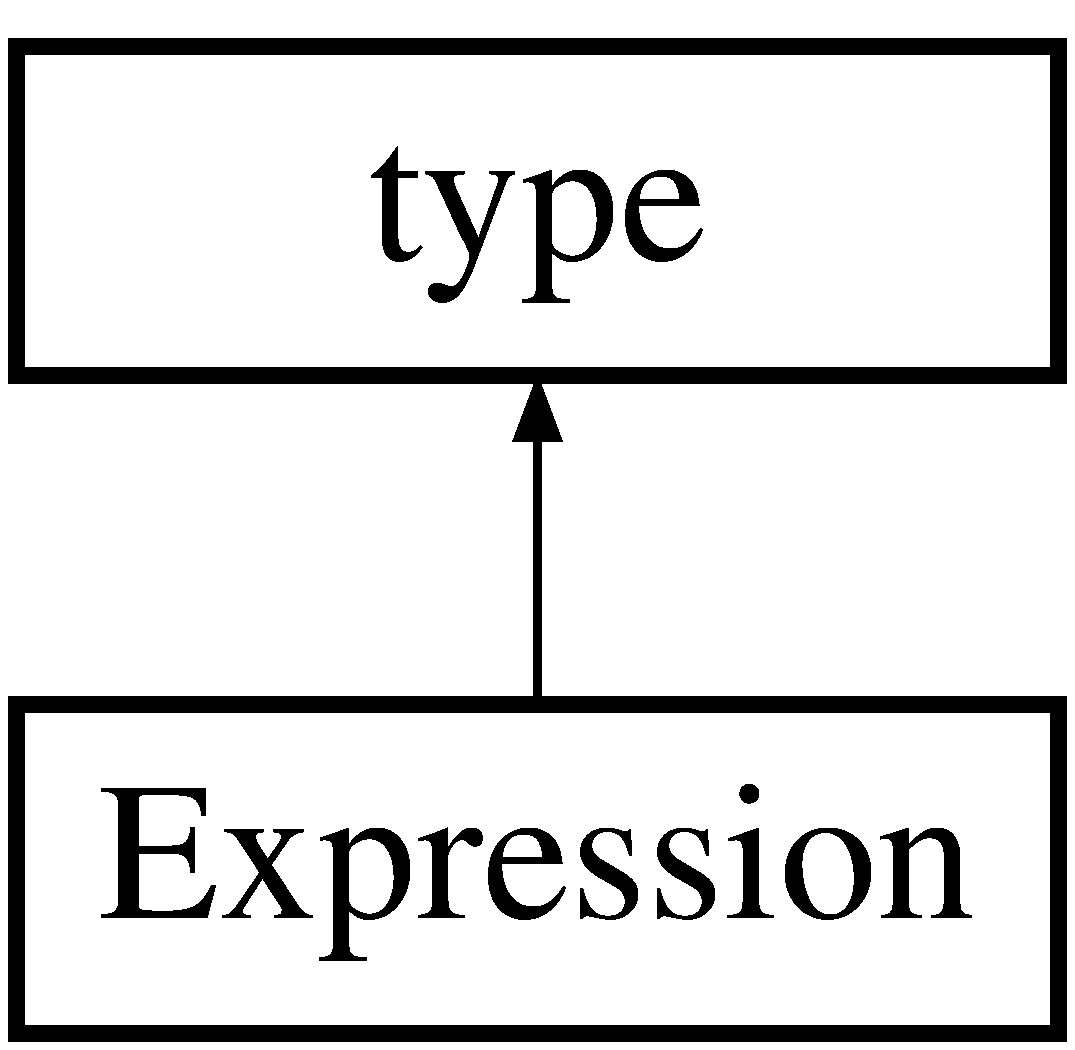
\includegraphics[height=2.000000cm]{class_expression}
\end{center}
\end{figure}
\subsection*{Public Member Functions}
\begin{DoxyCompactItemize}
\item 
\hyperlink{class_expression_a2dfc0f1fe384a18adb7064f44aca0bed}{Expression} (Q\-String \&exp1)
\begin{DoxyCompactList}\small\item\em Constructeur. \end{DoxyCompactList}\item 
\hyperlink{classtype}{type} $\ast$ \hyperlink{class_expression_a1572f9f1d8b2619b14d7d58f72a63e22}{operator+} (\hyperlink{classtype}{type} \&t)
\begin{DoxyCompactList}\small\item\em Operateur +. \end{DoxyCompactList}\item 
\hyperlink{classtype}{type} $\ast$ \hyperlink{class_expression_aeb3e786f0524b1b1e2c5b238c8d2e50c}{operator/} (\hyperlink{classtype}{type} \&t)
\begin{DoxyCompactList}\small\item\em Operateur /. \end{DoxyCompactList}\item 
\hyperlink{classtype}{type} $\ast$ \hyperlink{class_expression_a9f63512e41bb2e498951342759a6fa1e}{operator$\ast$} (\hyperlink{classtype}{type} \&t)
\begin{DoxyCompactList}\small\item\em Operateur $\ast$. \end{DoxyCompactList}\item 
\hyperlink{classtype}{type} $\ast$ \hyperlink{class_expression_adb495f245e3652e3605b290d7d41acb5}{operator-\/} (\hyperlink{classtype}{type} \&t)
\begin{DoxyCompactList}\small\item\em Operateur -\/. \end{DoxyCompactList}\item 
\hyperlink{classtype}{type} $\ast$ \hyperlink{class_expression_a67a5046f6af705fef094ff5e4a78880d}{sinus} (bool degre=false)
\begin{DoxyCompactList}\small\item\em Sinus. \end{DoxyCompactList}\item 
\hyperlink{classtype}{type} $\ast$ \hyperlink{class_expression_aeaf521221894a0012b604cc0033518b9}{pow} (\hyperlink{classtype}{type} \&t)
\begin{DoxyCompactList}\small\item\em Pow. \end{DoxyCompactList}\item 
\hyperlink{classtype}{type} $\ast$ \hyperlink{class_expression_ac46a4b88a1b08206e08da229fdbfd3e9}{mod} (\hyperlink{classtype}{type} \&t)
\begin{DoxyCompactList}\small\item\em mod \end{DoxyCompactList}\item 
\hyperlink{classtype}{type} $\ast$ \hyperlink{class_expression_aa654b4e71cfafd29af080020a77dc1e0}{sign} ()
\begin{DoxyCompactList}\small\item\em sign \end{DoxyCompactList}\item 
\hyperlink{classtype}{type} $\ast$ \hyperlink{class_expression_ab33831fb9207ba778ae46f49b2f0f7ac}{cosinus} (bool degre=false)
\begin{DoxyCompactList}\small\item\em Cosinus. \end{DoxyCompactList}\item 
\hyperlink{classtype}{type} $\ast$ \hyperlink{class_expression_ae47f82ffeefff823064141174ba5c3ac}{tangente} (bool degre=false)
\begin{DoxyCompactList}\small\item\em Tangente. \end{DoxyCompactList}\item 
\hyperlink{classtype}{type} $\ast$ \hyperlink{class_expression_a45aef44cb37e21e99614053bf80801f6}{sinush} (bool degre=false)
\begin{DoxyCompactList}\small\item\em Sinush. \end{DoxyCompactList}\item 
\hyperlink{classtype}{type} $\ast$ \hyperlink{class_expression_a032591ce129e8d11b9a75c55287323d8}{cosinush} (bool degre=false)
\begin{DoxyCompactList}\small\item\em Cosinush. \end{DoxyCompactList}\item 
\hyperlink{classtype}{type} $\ast$ \hyperlink{class_expression_a0d0acd016a909609e451836060d4e676}{tangenteh} (bool degre=false)
\begin{DoxyCompactList}\small\item\em Tangenteh. \end{DoxyCompactList}\item 
\hyperlink{classtype}{type} $\ast$ \hyperlink{class_expression_a1f6cd71d574995f2c3e80c3033ca2940}{ln} ()
\begin{DoxyCompactList}\small\item\em Ln. \end{DoxyCompactList}\item 
\hyperlink{classtype}{type} $\ast$ \hyperlink{class_expression_a9eb28aee26ef54093fc83f89ef3c1523}{log} ()
\begin{DoxyCompactList}\small\item\em Log. \end{DoxyCompactList}\item 
\hyperlink{classtype}{type} $\ast$ \hyperlink{class_expression_ab3dc93b84bb845663383b4347550c9d5}{inv} ()
\begin{DoxyCompactList}\small\item\em Inv. \end{DoxyCompactList}\item 
\hyperlink{classtype}{type} $\ast$ \hyperlink{class_expression_ac5b9d54cc3699ccec579001a9e954bd3}{sqrt} ()
\begin{DoxyCompactList}\small\item\em Sqrt. \end{DoxyCompactList}\item 
\hyperlink{classtype}{type} $\ast$ \hyperlink{class_expression_a172e59bd44c5ddf668fd8027f0733d8d}{sqr} ()
\begin{DoxyCompactList}\small\item\em Sqr. \end{DoxyCompactList}\item 
\hyperlink{classtype}{type} $\ast$ \hyperlink{class_expression_afaa9e88c0eedebcd346859b7593f5b48}{cube} ()
\begin{DoxyCompactList}\small\item\em Cube. \end{DoxyCompactList}\item 
Q\-String \hyperlink{class_expression_a7312cb958b6366f84fb4e01f58cd2119}{eval} ()
\begin{DoxyCompactList}\small\item\em eval \end{DoxyCompactList}\item 
Q\-String \hyperlink{class_expression_a4404792ff4997e7c06a3242062825f5c}{to\-Q\-String} ()
\begin{DoxyCompactList}\small\item\em to\-Q\-String \end{DoxyCompactList}\end{DoxyCompactItemize}
\subsection*{Additional Inherited Members}


\subsection{Detailed Description}
Classe representant une expression. 

La classe derive de type. Permet de representer une expression 

\subsection{Constructor \& Destructor Documentation}
\hypertarget{class_expression_a2dfc0f1fe384a18adb7064f44aca0bed}{\index{Expression@{Expression}!Expression@{Expression}}
\index{Expression@{Expression}!Expression@{Expression}}
\subsubsection[{Expression}]{\setlength{\rightskip}{0pt plus 5cm}Expression\-::\-Expression (
\begin{DoxyParamCaption}
\item[{Q\-String \&}]{exp1}
\end{DoxyParamCaption}
)}}\label{class_expression_a2dfc0f1fe384a18adb7064f44aca0bed}


Constructeur. 

Constructeur a partir de Qstring 
\begin{DoxyParams}{Parameters}
{\em exp1s} & \-: chaine source \\
\hline
\end{DoxyParams}


\subsection{Member Function Documentation}
\hypertarget{class_expression_ab33831fb9207ba778ae46f49b2f0f7ac}{\index{Expression@{Expression}!cosinus@{cosinus}}
\index{cosinus@{cosinus}!Expression@{Expression}}
\subsubsection[{cosinus}]{\setlength{\rightskip}{0pt plus 5cm}{\bf type} $\ast$ Expression\-::cosinus (
\begin{DoxyParamCaption}
\item[{bool}]{degre = {\ttfamily false}}
\end{DoxyParamCaption}
)\hspace{0.3cm}{\ttfamily [virtual]}}}\label{class_expression_ab33831fb9207ba778ae46f49b2f0f7ac}


Cosinus. 

Implementation de l'operateur unaire cosinus (methode virtuelle dans la classe mere) 
\begin{DoxyParams}{Parameters}
{\em degre} & \-: booleen, vrai si utilisation des degre, faux si utilisation des radians \\
\hline
\end{DoxyParams}
\begin{DoxyReturn}{Returns}
Pointeur sur type, resultat de l'operation 
\end{DoxyReturn}


Reimplemented from \hyperlink{classtype_a4bf0be87d5e0314cc6a29ce86930d34e}{type}.

\hypertarget{class_expression_a032591ce129e8d11b9a75c55287323d8}{\index{Expression@{Expression}!cosinush@{cosinush}}
\index{cosinush@{cosinush}!Expression@{Expression}}
\subsubsection[{cosinush}]{\setlength{\rightskip}{0pt plus 5cm}{\bf type} $\ast$ Expression\-::cosinush (
\begin{DoxyParamCaption}
\item[{bool}]{degre = {\ttfamily false}}
\end{DoxyParamCaption}
)\hspace{0.3cm}{\ttfamily [virtual]}}}\label{class_expression_a032591ce129e8d11b9a75c55287323d8}


Cosinush. 

Implementation de l'operateur unaire cosinush (methode virtuelle dans la classe mere) 
\begin{DoxyParams}{Parameters}
{\em degre} & \-: booleen, vrai si utilisation des degre, faux si utilisation des radians \\
\hline
\end{DoxyParams}
\begin{DoxyReturn}{Returns}
Pointeur sur type, resultat de l'operation 
\end{DoxyReturn}


Reimplemented from \hyperlink{classtype_a387836cc1a0dd2a20ece2f721fab822a}{type}.

\hypertarget{class_expression_afaa9e88c0eedebcd346859b7593f5b48}{\index{Expression@{Expression}!cube@{cube}}
\index{cube@{cube}!Expression@{Expression}}
\subsubsection[{cube}]{\setlength{\rightskip}{0pt plus 5cm}{\bf type} $\ast$ Expression\-::cube (
\begin{DoxyParamCaption}
{}
\end{DoxyParamCaption}
)\hspace{0.3cm}{\ttfamily [virtual]}}}\label{class_expression_afaa9e88c0eedebcd346859b7593f5b48}


Cube. 

Implementation de l'operateur unaire Cube (methode virtuelle dans la classe mere) \begin{DoxyReturn}{Returns}
Pointeur sur type, resultat de l'operation 
\end{DoxyReturn}


Reimplemented from \hyperlink{classtype_ac470662477ea88722b58e98fee3e1ec0}{type}.

\hypertarget{class_expression_a7312cb958b6366f84fb4e01f58cd2119}{\index{Expression@{Expression}!eval@{eval}}
\index{eval@{eval}!Expression@{Expression}}
\subsubsection[{eval}]{\setlength{\rightskip}{0pt plus 5cm}Q\-String Expression\-::eval (
\begin{DoxyParamCaption}
{}
\end{DoxyParamCaption}
)\hspace{0.3cm}{\ttfamily [virtual]}}}\label{class_expression_a7312cb958b6366f84fb4e01f58cd2119}


eval 

Implementation de l'operateur unaire eval (methode virtuelle dans la classe mere) \begin{DoxyReturn}{Returns}
Pointeur sur type, resultat de l'operation 
\end{DoxyReturn}


Reimplemented from \hyperlink{classtype_a8288e5361dba59212d1f2490f6531793}{type}.

\hypertarget{class_expression_ab3dc93b84bb845663383b4347550c9d5}{\index{Expression@{Expression}!inv@{inv}}
\index{inv@{inv}!Expression@{Expression}}
\subsubsection[{inv}]{\setlength{\rightskip}{0pt plus 5cm}{\bf type} $\ast$ Expression\-::inv (
\begin{DoxyParamCaption}
{}
\end{DoxyParamCaption}
)\hspace{0.3cm}{\ttfamily [virtual]}}}\label{class_expression_ab3dc93b84bb845663383b4347550c9d5}


Inv. 

Implementation de l'operateur unaire inv (methode virtuelle dans la classe mere) \begin{DoxyReturn}{Returns}
Pointeur sur type, resultat de l'operation 
\end{DoxyReturn}


Reimplemented from \hyperlink{classtype_af4bf1a878929fb77f6e1edf90d33a275}{type}.

\hypertarget{class_expression_a1f6cd71d574995f2c3e80c3033ca2940}{\index{Expression@{Expression}!ln@{ln}}
\index{ln@{ln}!Expression@{Expression}}
\subsubsection[{ln}]{\setlength{\rightskip}{0pt plus 5cm}{\bf type} $\ast$ Expression\-::ln (
\begin{DoxyParamCaption}
{}
\end{DoxyParamCaption}
)\hspace{0.3cm}{\ttfamily [virtual]}}}\label{class_expression_a1f6cd71d574995f2c3e80c3033ca2940}


Ln. 

Implementation de l'operateur unaire ln (methode virtuelle dans la classe mere) \begin{DoxyReturn}{Returns}
Pointeur sur type, resultat de l'operation 
\end{DoxyReturn}


Reimplemented from \hyperlink{classtype_aba57b52b37f984806842df5478b2489c}{type}.

\hypertarget{class_expression_a9eb28aee26ef54093fc83f89ef3c1523}{\index{Expression@{Expression}!log@{log}}
\index{log@{log}!Expression@{Expression}}
\subsubsection[{log}]{\setlength{\rightskip}{0pt plus 5cm}{\bf type} $\ast$ Expression\-::log (
\begin{DoxyParamCaption}
{}
\end{DoxyParamCaption}
)\hspace{0.3cm}{\ttfamily [virtual]}}}\label{class_expression_a9eb28aee26ef54093fc83f89ef3c1523}


Log. 

Implementation de l'operateur unaire log (methode virtuelle dans la classe mere) \begin{DoxyReturn}{Returns}
Pointeur sur type, resultat de l'operation 
\end{DoxyReturn}


Reimplemented from \hyperlink{classtype_ab02a7131b07f81a545beb9ae499bcef6}{type}.

\hypertarget{class_expression_ac46a4b88a1b08206e08da229fdbfd3e9}{\index{Expression@{Expression}!mod@{mod}}
\index{mod@{mod}!Expression@{Expression}}
\subsubsection[{mod}]{\setlength{\rightskip}{0pt plus 5cm}{\bf type} $\ast$ Expression\-::mod (
\begin{DoxyParamCaption}
\item[{{\bf type} \&}]{t}
\end{DoxyParamCaption}
)\hspace{0.3cm}{\ttfamily [virtual]}}}\label{class_expression_ac46a4b88a1b08206e08da229fdbfd3e9}


mod 

Implementation de l'operateur binaire modulo (methode virtuelle dans la classe mere) \begin{DoxyReturn}{Returns}
Pointeur sur type, resultat de l'operation 
\end{DoxyReturn}


Reimplemented from \hyperlink{classtype_aed752df353b43b17d3f993d4b02f216b}{type}.

\hypertarget{class_expression_a9f63512e41bb2e498951342759a6fa1e}{\index{Expression@{Expression}!operator$\ast$@{operator$\ast$}}
\index{operator$\ast$@{operator$\ast$}!Expression@{Expression}}
\subsubsection[{operator$\ast$}]{\setlength{\rightskip}{0pt plus 5cm}{\bf type} $\ast$ Expression\-::operator$\ast$ (
\begin{DoxyParamCaption}
\item[{{\bf type} \&}]{t}
\end{DoxyParamCaption}
)\hspace{0.3cm}{\ttfamily [virtual]}}}\label{class_expression_a9f63512e41bb2e498951342759a6fa1e}


Operateur $\ast$. 

Implementation de l'operateur binaire $\ast$ (methode virtuelle dans la classe mere) 
\begin{DoxyParams}{Parameters}
{\em t} & \-: Pointeur sur un type \\
\hline
\end{DoxyParams}
\begin{DoxyReturn}{Returns}
Pointeur sur type, resultat de l'operation 
\end{DoxyReturn}


Implements \hyperlink{classtype_a9e275d2b8465d6085515f58aaf631ea7}{type}.

\hypertarget{class_expression_a1572f9f1d8b2619b14d7d58f72a63e22}{\index{Expression@{Expression}!operator+@{operator+}}
\index{operator+@{operator+}!Expression@{Expression}}
\subsubsection[{operator+}]{\setlength{\rightskip}{0pt plus 5cm}{\bf type} $\ast$ Expression\-::operator+ (
\begin{DoxyParamCaption}
\item[{{\bf type} \&}]{t}
\end{DoxyParamCaption}
)\hspace{0.3cm}{\ttfamily [virtual]}}}\label{class_expression_a1572f9f1d8b2619b14d7d58f72a63e22}


Operateur +. 

Implementation de l'operateur binaire + (methode virtuelle dans la classe mere) 
\begin{DoxyParams}{Parameters}
{\em t} & \-: Pointeur sur un type \\
\hline
\end{DoxyParams}
\begin{DoxyReturn}{Returns}
Pointeur sur type, resultat de l'operation 
\end{DoxyReturn}


Implements \hyperlink{classtype_aae435de533d21af297434702fd71d04d}{type}.

\hypertarget{class_expression_adb495f245e3652e3605b290d7d41acb5}{\index{Expression@{Expression}!operator-\/@{operator-\/}}
\index{operator-\/@{operator-\/}!Expression@{Expression}}
\subsubsection[{operator-\/}]{\setlength{\rightskip}{0pt plus 5cm}{\bf type} $\ast$ Expression\-::operator-\/ (
\begin{DoxyParamCaption}
\item[{{\bf type} \&}]{t}
\end{DoxyParamCaption}
)\hspace{0.3cm}{\ttfamily [virtual]}}}\label{class_expression_adb495f245e3652e3605b290d7d41acb5}


Operateur -\/. 

Implementation de l'operateur binaire -\/ (methode virtuelle dans la classe mere) 
\begin{DoxyParams}{Parameters}
{\em t} & \-: Pointeur sur un type \\
\hline
\end{DoxyParams}
\begin{DoxyReturn}{Returns}
Pointeur sur type, resultat de l'operation 
\end{DoxyReturn}


Implements \hyperlink{classtype_a4d440ee89d624d7314786d8d18751588}{type}.

\hypertarget{class_expression_aeb3e786f0524b1b1e2c5b238c8d2e50c}{\index{Expression@{Expression}!operator/@{operator/}}
\index{operator/@{operator/}!Expression@{Expression}}
\subsubsection[{operator/}]{\setlength{\rightskip}{0pt plus 5cm}{\bf type} $\ast$ Expression\-::operator/ (
\begin{DoxyParamCaption}
\item[{{\bf type} \&}]{t}
\end{DoxyParamCaption}
)\hspace{0.3cm}{\ttfamily [virtual]}}}\label{class_expression_aeb3e786f0524b1b1e2c5b238c8d2e50c}


Operateur /. 

Implementation de l'operateur binaire / (methode virtuelle dans la classe mere) 
\begin{DoxyParams}{Parameters}
{\em t} & \-: Pointeur sur un type \\
\hline
\end{DoxyParams}
\begin{DoxyReturn}{Returns}
Pointeur sur type, resultat de l'operation 
\end{DoxyReturn}


Implements \hyperlink{classtype_a0fad8179d45b9bbde90b48e1950ce639}{type}.

\hypertarget{class_expression_aeaf521221894a0012b604cc0033518b9}{\index{Expression@{Expression}!pow@{pow}}
\index{pow@{pow}!Expression@{Expression}}
\subsubsection[{pow}]{\setlength{\rightskip}{0pt plus 5cm}{\bf type} $\ast$ Expression\-::pow (
\begin{DoxyParamCaption}
\item[{{\bf type} \&}]{t}
\end{DoxyParamCaption}
)\hspace{0.3cm}{\ttfamily [virtual]}}}\label{class_expression_aeaf521221894a0012b604cc0033518b9}


Pow. 

Implementation de l'operateur binaire pow (methode virtuelle dans la classe mere) 
\begin{DoxyParams}{Parameters}
{\em t} & \-: Pointeur sur un type \\
\hline
\end{DoxyParams}
\begin{DoxyReturn}{Returns}
Pointeur sur type, resultat de l'operation 
\end{DoxyReturn}


Reimplemented from \hyperlink{classtype_a01ae853856fcd929e5455b460ccd0be6}{type}.

\hypertarget{class_expression_aa654b4e71cfafd29af080020a77dc1e0}{\index{Expression@{Expression}!sign@{sign}}
\index{sign@{sign}!Expression@{Expression}}
\subsubsection[{sign}]{\setlength{\rightskip}{0pt plus 5cm}{\bf type} $\ast$ Expression\-::sign (
\begin{DoxyParamCaption}
{}
\end{DoxyParamCaption}
)\hspace{0.3cm}{\ttfamily [virtual]}}}\label{class_expression_aa654b4e71cfafd29af080020a77dc1e0}


sign 

Implementation de l'operateur unaire sign (methode virtuelle dans la classe mere) Inverse le signe de la constante \begin{DoxyReturn}{Returns}
Pointeur sur type, resultat de l'operation 
\end{DoxyReturn}


Reimplemented from \hyperlink{classtype_a3ec9f31aec3ddc52efe2adff634a671a}{type}.

\hypertarget{class_expression_a67a5046f6af705fef094ff5e4a78880d}{\index{Expression@{Expression}!sinus@{sinus}}
\index{sinus@{sinus}!Expression@{Expression}}
\subsubsection[{sinus}]{\setlength{\rightskip}{0pt plus 5cm}{\bf type} $\ast$ Expression\-::sinus (
\begin{DoxyParamCaption}
\item[{bool}]{degre = {\ttfamily false}}
\end{DoxyParamCaption}
)\hspace{0.3cm}{\ttfamily [virtual]}}}\label{class_expression_a67a5046f6af705fef094ff5e4a78880d}


Sinus. 

Implementation de l'operateur unaire sinus (methode virtuelle dans la classe mere) 
\begin{DoxyParams}{Parameters}
{\em degre} & \-: booleen, vrai si utilisation des degre, faux si utilisation des radians \\
\hline
\end{DoxyParams}
\begin{DoxyReturn}{Returns}
Pointeur sur type, resultat de l'operation 
\end{DoxyReturn}


Reimplemented from \hyperlink{classtype_acfff98100e9af7fe51f22ca553b49652}{type}.

\hypertarget{class_expression_a45aef44cb37e21e99614053bf80801f6}{\index{Expression@{Expression}!sinush@{sinush}}
\index{sinush@{sinush}!Expression@{Expression}}
\subsubsection[{sinush}]{\setlength{\rightskip}{0pt plus 5cm}{\bf type} $\ast$ Expression\-::sinush (
\begin{DoxyParamCaption}
\item[{bool}]{degre = {\ttfamily false}}
\end{DoxyParamCaption}
)\hspace{0.3cm}{\ttfamily [virtual]}}}\label{class_expression_a45aef44cb37e21e99614053bf80801f6}


Sinush. 

Implementation de l'operateur unaire sinush (methode virtuelle dans la classe mere) 
\begin{DoxyParams}{Parameters}
{\em degre} & \-: booleen, vrai si utilisation des degre, faux si utilisation des radians \\
\hline
\end{DoxyParams}
\begin{DoxyReturn}{Returns}
Pointeur sur type, resultat de l'operation 
\end{DoxyReturn}


Reimplemented from \hyperlink{classtype_a1bb104502962725e2d8d1909a208e7fa}{type}.

\hypertarget{class_expression_a172e59bd44c5ddf668fd8027f0733d8d}{\index{Expression@{Expression}!sqr@{sqr}}
\index{sqr@{sqr}!Expression@{Expression}}
\subsubsection[{sqr}]{\setlength{\rightskip}{0pt plus 5cm}{\bf type} $\ast$ Expression\-::sqr (
\begin{DoxyParamCaption}
{}
\end{DoxyParamCaption}
)\hspace{0.3cm}{\ttfamily [virtual]}}}\label{class_expression_a172e59bd44c5ddf668fd8027f0733d8d}


Sqr. 

Implementation de l'operateur unaire sqr (methode virtuelle dans la classe mere) \begin{DoxyReturn}{Returns}
Pointeur sur type, resultat de l'operation 
\end{DoxyReturn}


Reimplemented from \hyperlink{classtype_a70b655b274b3378154cd29127c22a4f0}{type}.

\hypertarget{class_expression_ac5b9d54cc3699ccec579001a9e954bd3}{\index{Expression@{Expression}!sqrt@{sqrt}}
\index{sqrt@{sqrt}!Expression@{Expression}}
\subsubsection[{sqrt}]{\setlength{\rightskip}{0pt plus 5cm}{\bf type} $\ast$ Expression\-::sqrt (
\begin{DoxyParamCaption}
{}
\end{DoxyParamCaption}
)\hspace{0.3cm}{\ttfamily [virtual]}}}\label{class_expression_ac5b9d54cc3699ccec579001a9e954bd3}


Sqrt. 

Implementation de l'operateur unaire sqrt (methode virtuelle dans la classe mere) \begin{DoxyReturn}{Returns}
Pointeur sur type, resultat de l'operation 
\end{DoxyReturn}


Reimplemented from \hyperlink{classtype_aedd0df2ba42b6cb66ee3dba28309a47b}{type}.

\hypertarget{class_expression_ae47f82ffeefff823064141174ba5c3ac}{\index{Expression@{Expression}!tangente@{tangente}}
\index{tangente@{tangente}!Expression@{Expression}}
\subsubsection[{tangente}]{\setlength{\rightskip}{0pt plus 5cm}{\bf type} $\ast$ Expression\-::tangente (
\begin{DoxyParamCaption}
\item[{bool}]{degre = {\ttfamily false}}
\end{DoxyParamCaption}
)\hspace{0.3cm}{\ttfamily [virtual]}}}\label{class_expression_ae47f82ffeefff823064141174ba5c3ac}


Tangente. 

Implementation de l'operateur unaire tangente (methode virtuelle dans la classe mere) 
\begin{DoxyParams}{Parameters}
{\em degre} & \-: booleen, vrai si utilisation des degre, faux si utilisation des radians \\
\hline
\end{DoxyParams}
\begin{DoxyReturn}{Returns}
Pointeur sur type, resultat de l'operation 
\end{DoxyReturn}


Reimplemented from \hyperlink{classtype_a0e48cd1a39419994f14550b2fd188e1d}{type}.

\hypertarget{class_expression_a0d0acd016a909609e451836060d4e676}{\index{Expression@{Expression}!tangenteh@{tangenteh}}
\index{tangenteh@{tangenteh}!Expression@{Expression}}
\subsubsection[{tangenteh}]{\setlength{\rightskip}{0pt plus 5cm}{\bf type} $\ast$ Expression\-::tangenteh (
\begin{DoxyParamCaption}
\item[{bool}]{degre = {\ttfamily false}}
\end{DoxyParamCaption}
)\hspace{0.3cm}{\ttfamily [virtual]}}}\label{class_expression_a0d0acd016a909609e451836060d4e676}


Tangenteh. 

Implementation de l'operateur unaire tangenteh (methode virtuelle dans la classe mere) 
\begin{DoxyParams}{Parameters}
{\em degre} & \-: booleen, vrai si utilisation des degre, faux si utilisation des radians \\
\hline
\end{DoxyParams}
\begin{DoxyReturn}{Returns}
Pointeur sur type, resultat de l'operation 
\end{DoxyReturn}


Reimplemented from \hyperlink{classtype_a36763dd363a8de97e4a52aa87776e61c}{type}.

\hypertarget{class_expression_a4404792ff4997e7c06a3242062825f5c}{\index{Expression@{Expression}!to\-Q\-String@{to\-Q\-String}}
\index{to\-Q\-String@{to\-Q\-String}!Expression@{Expression}}
\subsubsection[{to\-Q\-String}]{\setlength{\rightskip}{0pt plus 5cm}Q\-String Expression\-::to\-Q\-String (
\begin{DoxyParamCaption}
{}
\end{DoxyParamCaption}
)\hspace{0.3cm}{\ttfamily [inline]}, {\ttfamily [virtual]}}}\label{class_expression_a4404792ff4997e7c06a3242062825f5c}


to\-Q\-String 

Transforme l'objet Qstring. Permet ensuite l'affichage dans des widget \begin{DoxyReturn}{Returns}
Qstring \-: chaine resultat 
\end{DoxyReturn}


Implements \hyperlink{classtype_ab61f01d56f3896cc99788a1a18c4b0c2}{type}.



The documentation for this class was generated from the following files\-:\begin{DoxyCompactItemize}
\item 
Code/projet\-\_\-lo21/\hyperlink{expression_8h}{expression.\-h}\item 
Code/projet\-\_\-lo21/expression.\-cpp\end{DoxyCompactItemize}

\hypertarget{classgardien}{\section{gardien Class Reference}
\label{classgardien}\index{gardien@{gardien}}
}


{\ttfamily \#include $<$gardien.\-h$>$}

\subsection*{Public Member Functions}
\begin{DoxyCompactItemize}
\item 
\hyperlink{classgardien_a23b498d98e7a90384585f9d3721b29fe}{gardien} ()
\item 
\hyperlink{class_pile}{Pile} $\ast$ \hyperlink{classgardien_a766daaa5df48bed986a03f188c8de4e0}{undo} ()
\item 
\hyperlink{class_pile}{Pile} $\ast$ \hyperlink{classgardien_a2c4455417103371b0281a01e32ac77fc}{redo} ()
\item 
void \hyperlink{classgardien_a71a30cc54cd294ff17425a0bb55504e1}{add\-Memento} (\hyperlink{class_pile}{Pile} pile)
\end{DoxyCompactItemize}


\subsection{Constructor \& Destructor Documentation}
\hypertarget{classgardien_a23b498d98e7a90384585f9d3721b29fe}{\index{gardien@{gardien}!gardien@{gardien}}
\index{gardien@{gardien}!gardien@{gardien}}
\subsubsection[{gardien}]{\setlength{\rightskip}{0pt plus 5cm}gardien\-::gardien (
\begin{DoxyParamCaption}
{}
\end{DoxyParamCaption}
)}}\label{classgardien_a23b498d98e7a90384585f9d3721b29fe}


\subsection{Member Function Documentation}
\hypertarget{classgardien_a71a30cc54cd294ff17425a0bb55504e1}{\index{gardien@{gardien}!add\-Memento@{add\-Memento}}
\index{add\-Memento@{add\-Memento}!gardien@{gardien}}
\subsubsection[{add\-Memento}]{\setlength{\rightskip}{0pt plus 5cm}void gardien\-::add\-Memento (
\begin{DoxyParamCaption}
\item[{{\bf Pile}}]{pile}
\end{DoxyParamCaption}
)}}\label{classgardien_a71a30cc54cd294ff17425a0bb55504e1}
\hypertarget{classgardien_a2c4455417103371b0281a01e32ac77fc}{\index{gardien@{gardien}!redo@{redo}}
\index{redo@{redo}!gardien@{gardien}}
\subsubsection[{redo}]{\setlength{\rightskip}{0pt plus 5cm}{\bf Pile} $\ast$ gardien\-::redo (
\begin{DoxyParamCaption}
{}
\end{DoxyParamCaption}
)}}\label{classgardien_a2c4455417103371b0281a01e32ac77fc}
\hypertarget{classgardien_a766daaa5df48bed986a03f188c8de4e0}{\index{gardien@{gardien}!undo@{undo}}
\index{undo@{undo}!gardien@{gardien}}
\subsubsection[{undo}]{\setlength{\rightskip}{0pt plus 5cm}{\bf Pile} $\ast$ gardien\-::undo (
\begin{DoxyParamCaption}
{}
\end{DoxyParamCaption}
)}}\label{classgardien_a766daaa5df48bed986a03f188c8de4e0}


The documentation for this class was generated from the following files\-:\begin{DoxyCompactItemize}
\item 
Code/projet\-\_\-lo21/\hyperlink{gardien_8h}{gardien.\-h}\item 
Code/projet\-\_\-lo21/\hyperlink{gardien_8cpp}{gardien.\-cpp}\end{DoxyCompactItemize}

\hypertarget{class_main_window}{\section{Main\-Window Class Reference}
\label{class_main_window}\index{Main\-Window@{Main\-Window}}
}


Classe gerant l'affichage.  




{\ttfamily \#include $<$mainwindow.\-h$>$}

\subsection*{Signals}
\begin{DoxyCompactItemize}
\item 
\hypertarget{class_main_window_a1e39eccc1e017799bda6b446b8280edf}{void {\bfseries push\-Stack\-\_\-signal} (const Q\-String \&)}\label{class_main_window_a1e39eccc1e017799bda6b446b8280edf}

\item 
\hypertarget{class_main_window_aed37073752de791b6ad06e41a8e9f1b2}{void {\bfseries clean\-List\-\_\-signal} ()}\label{class_main_window_aed37073752de791b6ad06e41a8e9f1b2}

\item 
\hypertarget{class_main_window_a94d40675237489fc9d25ccc868a4dcbd}{void {\bfseries refresh\-\_\-signal} ()}\label{class_main_window_a94d40675237489fc9d25ccc868a4dcbd}

\end{DoxyCompactItemize}
\subsection*{Public Member Functions}
\begin{DoxyCompactItemize}
\item 
\hypertarget{class_main_window_ac8603055e732d11c01cfa8e44bff3ca2}{{\bfseries Main\-Window} (\hyperlink{class_pile}{Pile} \&pile, Q\-Widget $\ast$parent)}\label{class_main_window_ac8603055e732d11c01cfa8e44bff3ca2}

\end{DoxyCompactItemize}


\subsection{Detailed Description}
Classe gerant l'affichage. 

The documentation for this class was generated from the following files\-:\begin{DoxyCompactItemize}
\item 
Code/projet\-\_\-lo21/\hyperlink{mainwindow_8h}{mainwindow.\-h}\item 
Code/projet\-\_\-lo21/mainwindow.\-cpp\end{DoxyCompactItemize}

\hypertarget{classnocomplex}{\section{nocomplex Class Reference}
\label{classnocomplex}\index{nocomplex@{nocomplex}}
}


{\ttfamily \#include $<$nocomplex.\-h$>$}



Inherits \hyperlink{classconstante}{constante}.



Inherited by \hyperlink{classentier}{entier}, \hyperlink{classrationnel}{rationnel}, and \hyperlink{classreel}{reel}.

\subsection*{Public Member Functions}
\begin{DoxyCompactItemize}
\item 
\hyperlink{classnocomplex_a633b5bd1a8681544bb2773605cffed9c}{nocomplex} ()
\item 
virtual \hyperlink{classtype}{type} $\ast$ \hyperlink{classnocomplex_af3d04b00f4f82d3a35cad0ca023093f4}{operator+} (\hyperlink{classtype}{type} \&t)=0
\item 
virtual \hyperlink{classtype}{type} $\ast$ \hyperlink{classnocomplex_a47942bdcc78cfc5d5e867c9f9836a465}{operator/} (\hyperlink{classtype}{type} \&t)=0
\item 
virtual \hyperlink{classtype}{type} $\ast$ \hyperlink{classnocomplex_ac84954cbe0bd9c77eab88c0b97b34c2b}{operator$\ast$} (\hyperlink{classtype}{type} \&t)=0
\item 
virtual \hyperlink{classtype}{type} $\ast$ \hyperlink{classnocomplex_a2005c3a0fcaa1f360561539931ffc578}{operator-\/} (\hyperlink{classtype}{type} \&t)=0
\end{DoxyCompactItemize}


\subsection{Constructor \& Destructor Documentation}
\hypertarget{classnocomplex_a633b5bd1a8681544bb2773605cffed9c}{\index{nocomplex@{nocomplex}!nocomplex@{nocomplex}}
\index{nocomplex@{nocomplex}!nocomplex@{nocomplex}}
\subsubsection[{nocomplex}]{\setlength{\rightskip}{0pt plus 5cm}nocomplex\-::nocomplex (
\begin{DoxyParamCaption}
{}
\end{DoxyParamCaption}
)\hspace{0.3cm}{\ttfamily [inline]}}}\label{classnocomplex_a633b5bd1a8681544bb2773605cffed9c}


\subsection{Member Function Documentation}
\hypertarget{classnocomplex_ac84954cbe0bd9c77eab88c0b97b34c2b}{\index{nocomplex@{nocomplex}!operator$\ast$@{operator$\ast$}}
\index{operator$\ast$@{operator$\ast$}!nocomplex@{nocomplex}}
\subsubsection[{operator$\ast$}]{\setlength{\rightskip}{0pt plus 5cm}virtual {\bf type}$\ast$ nocomplex\-::operator$\ast$ (
\begin{DoxyParamCaption}
\item[{{\bf type} \&}]{t}
\end{DoxyParamCaption}
)\hspace{0.3cm}{\ttfamily [pure virtual]}}}\label{classnocomplex_ac84954cbe0bd9c77eab88c0b97b34c2b}


Implements \hyperlink{classtype_a9e275d2b8465d6085515f58aaf631ea7}{type}.



Implemented in \hyperlink{classreel_a044791a71fd9926cbedf3f19f6eea122}{reel}, \hyperlink{classentier_a7314a5aad4a2c997eaea01e3aa42092a}{entier}, and \hyperlink{classrationnel_a49250cb9001aad230e5193515ee74efa}{rationnel}.

\hypertarget{classnocomplex_af3d04b00f4f82d3a35cad0ca023093f4}{\index{nocomplex@{nocomplex}!operator+@{operator+}}
\index{operator+@{operator+}!nocomplex@{nocomplex}}
\subsubsection[{operator+}]{\setlength{\rightskip}{0pt plus 5cm}virtual {\bf type}$\ast$ nocomplex\-::operator+ (
\begin{DoxyParamCaption}
\item[{{\bf type} \&}]{t}
\end{DoxyParamCaption}
)\hspace{0.3cm}{\ttfamily [pure virtual]}}}\label{classnocomplex_af3d04b00f4f82d3a35cad0ca023093f4}


Implements \hyperlink{classtype_aae435de533d21af297434702fd71d04d}{type}.



Implemented in \hyperlink{classrationnel_a14d9d411058e146e075ccf16997e525e}{rationnel}, \hyperlink{classreel_af2ae884e68ab28b286cf9940f05f59d9}{reel}, and \hyperlink{classentier_a531e654172d6e2fe225fad108dbb84a7}{entier}.

\hypertarget{classnocomplex_a2005c3a0fcaa1f360561539931ffc578}{\index{nocomplex@{nocomplex}!operator-\/@{operator-\/}}
\index{operator-\/@{operator-\/}!nocomplex@{nocomplex}}
\subsubsection[{operator-\/}]{\setlength{\rightskip}{0pt plus 5cm}virtual {\bf type}$\ast$ nocomplex\-::operator-\/ (
\begin{DoxyParamCaption}
\item[{{\bf type} \&}]{t}
\end{DoxyParamCaption}
)\hspace{0.3cm}{\ttfamily [pure virtual]}}}\label{classnocomplex_a2005c3a0fcaa1f360561539931ffc578}


Implements \hyperlink{classtype_a4d440ee89d624d7314786d8d18751588}{type}.



Implemented in \hyperlink{classreel_a9cd96b762004392eda5216262201322c}{reel}, \hyperlink{classentier_ac0acf2b6156ef6f5f2e034c0425e1114}{entier}, and \hyperlink{classrationnel_a3bdf6de1a2526ddafbf1831a9af11dc9}{rationnel}.

\hypertarget{classnocomplex_a47942bdcc78cfc5d5e867c9f9836a465}{\index{nocomplex@{nocomplex}!operator/@{operator/}}
\index{operator/@{operator/}!nocomplex@{nocomplex}}
\subsubsection[{operator/}]{\setlength{\rightskip}{0pt plus 5cm}virtual {\bf type}$\ast$ nocomplex\-::operator/ (
\begin{DoxyParamCaption}
\item[{{\bf type} \&}]{t}
\end{DoxyParamCaption}
)\hspace{0.3cm}{\ttfamily [pure virtual]}}}\label{classnocomplex_a47942bdcc78cfc5d5e867c9f9836a465}


Implements \hyperlink{classtype_a0fad8179d45b9bbde90b48e1950ce639}{type}.



Implemented in \hyperlink{classreel_a3bc55f29b377547040d47be018b73fe6}{reel}, \hyperlink{classrationnel_ae36b04407cc70d425ed0292975b0d1e9}{rationnel}, and \hyperlink{classentier_a3bfd34b6998c5c09df0dbbadead47867}{entier}.



The documentation for this class was generated from the following file\-:\begin{DoxyCompactItemize}
\item 
Code/projet\-\_\-lo21/\hyperlink{nocomplex_8h}{nocomplex.\-h}\end{DoxyCompactItemize}

\hypertarget{class_pile}{\section{Pile Class Reference}
\label{class_pile}\index{Pile@{Pile}}
}


{\ttfamily \#include $<$pile.\-h$>$}

\subsection*{Public Member Functions}
\begin{DoxyCompactItemize}
\item 
\hyperlink{class_pile_ab2d1398d675586ff34994e2b109df152}{$\sim$\-Pile} ()
\item 
\hyperlink{class_pile_ab44e927107b28f5f3ac7697d10e0a739}{Pile} ()
\item 
\hyperlink{class_pile}{Pile} \& \hyperlink{class_pile_a13e1620ba0de2d1cd4b1f66f5356a8b4}{clone} () const 
\item 
\hyperlink{class_pile}{Pile} \& \hyperlink{class_pile_aee5282e29d14470c8805b62830207306}{duplique} () const 
\item 
void \hyperlink{class_pile_aace6210d258170c7420d6a4bda5ec967}{set\-Gardien} (\hyperlink{classgardien}{gardien} $\ast$\-\_\-g)
\item 
void \hyperlink{class_pile_a09fd751d9d6d0d3c861f97405756db56}{set\-Nb\-Elt} (int nb)
\item 
\hyperlink{classgardien}{gardien} $\ast$ \hyperlink{class_pile_af610383f7aa4076d56646753de61bdc6}{get\-Gardien} () const 
\item 
void \hyperlink{class_pile_a667e4bd3ec87f598cac5f5c761bd1623}{swap} (const unsigned int x, const unsigned int y)
\item 
void \hyperlink{class_pile_ab2671569b6870d06fb94179e998e2e2e}{sum} (const unsigned int x)
\item 
void \hyperlink{class_pile_a3993e0e33e78011663b15b9eb723d456}{mean} (const unsigned int x)
\item 
void \hyperlink{class_pile_a081f7843d01cae1f0f7be7d92e46d5d2}{dup} ()
\item 
void \hyperlink{class_pile_a7488ed257c6ceb16ed57a9fffb0726d5}{drop} ()
\item 
void \hyperlink{class_pile_a2f7afa189e97a23a836f07f9898538cf}{addition} ()
\item 
void \hyperlink{class_pile_ab1827b113fff2c3fa59ebbe4c5902b1b}{soustraction} ()
\item 
void \hyperlink{class_pile_a48ef99542609f5033f58ebd23189f698}{division} ()
\item 
void \hyperlink{class_pile_ae5006ad08419fc6dcf65cbb4970199fe}{multiplication} ()
\item 
void \hyperlink{class_pile_ac0be84cde5594e29678125e600bd8898}{parser} (Q\-String s)
\item 
int \hyperlink{class_pile_acc36fadfcc65c9863a9d1d8d5dbe859a}{get\-Nb} ()
\item 
void \hyperlink{class_pile_af91a4b277236024aa5aab9ef410881bb}{undo} ()
\item 
void \hyperlink{class_pile_aa8319a2921d86236d135cff700a5f833}{redo} ()
\item 
void \hyperlink{class_pile_a20b1ece0cc61ecefc78e1a785ad8235f}{pow} ()
\item 
void \hyperlink{class_pile_a6d6092af4859ea5cefaa7959bb208774}{mod} ()
\item 
void \hyperlink{class_pile_ad6ce16606725f1b2fa1028073afc3b75}{sign} ()
\item 
void \hyperlink{class_pile_a3a55c324834f3c6a194fce721492748a}{sinus} ()
\item 
void \hyperlink{class_pile_a338ae80ae690356ce13d3e065fb61a4a}{cosinus} ()
\item 
void \hyperlink{class_pile_ac41a978af4eeff70aafccbfc5b1d865f}{tangente} ()
\item 
void \hyperlink{class_pile_aaf8dcd15ed6a1af20a451c67b4aa0431}{sinush} ()
\item 
void \hyperlink{class_pile_a4e5e6d1bc818b0f947e12c5ff7049094}{cosinush} ()
\item 
void \hyperlink{class_pile_acb89de235850fdc79448fa40506eb20e}{tangenteh} ()
\item 
void \hyperlink{class_pile_ab22aed5e5178d32a3e47d8f4c599c9c4}{ln} ()
\item 
void \hyperlink{class_pile_acaec5142e3afb5208091eecb6ac31f35}{log} ()
\item 
void \hyperlink{class_pile_a040844b7b06a3aa8a25c47079858e5d4}{inv} ()
\item 
void \hyperlink{class_pile_a15e52c1dca0ef1e78af39c69f814e01a}{sqrt} ()
\item 
void \hyperlink{class_pile_abd1c5a18cb8dd304e377d74fcec5a513}{sqr} ()
\item 
void \hyperlink{class_pile_aee724c6620382459f78fab4fb08749eb}{cube} ()
\item 
void \hyperlink{class_pile_a582a24a17a82fc63985900765b0499b4}{fact} ()
\item 
void \hyperlink{class_pile_a9fbff00a90c14aca3b093b080c8b0f0b}{eval} ()
\end{DoxyCompactItemize}


\subsection{Constructor \& Destructor Documentation}
\hypertarget{class_pile_ab2d1398d675586ff34994e2b109df152}{\index{Pile@{Pile}!$\sim$\-Pile@{$\sim$\-Pile}}
\index{$\sim$\-Pile@{$\sim$\-Pile}!Pile@{Pile}}
\subsubsection[{$\sim$\-Pile}]{\setlength{\rightskip}{0pt plus 5cm}Pile\-::$\sim$\-Pile (
\begin{DoxyParamCaption}
{}
\end{DoxyParamCaption}
)}}\label{class_pile_ab2d1398d675586ff34994e2b109df152}
\hypertarget{class_pile_ab44e927107b28f5f3ac7697d10e0a739}{\index{Pile@{Pile}!Pile@{Pile}}
\index{Pile@{Pile}!Pile@{Pile}}
\subsubsection[{Pile}]{\setlength{\rightskip}{0pt plus 5cm}Pile\-::\-Pile (
\begin{DoxyParamCaption}
{}
\end{DoxyParamCaption}
)}}\label{class_pile_ab44e927107b28f5f3ac7697d10e0a739}


\subsection{Member Function Documentation}
\hypertarget{class_pile_a2f7afa189e97a23a836f07f9898538cf}{\index{Pile@{Pile}!addition@{addition}}
\index{addition@{addition}!Pile@{Pile}}
\subsubsection[{addition}]{\setlength{\rightskip}{0pt plus 5cm}void Pile\-::addition (
\begin{DoxyParamCaption}
{}
\end{DoxyParamCaption}
)}}\label{class_pile_a2f7afa189e97a23a836f07f9898538cf}
\hypertarget{class_pile_a13e1620ba0de2d1cd4b1f66f5356a8b4}{\index{Pile@{Pile}!clone@{clone}}
\index{clone@{clone}!Pile@{Pile}}
\subsubsection[{clone}]{\setlength{\rightskip}{0pt plus 5cm}{\bf Pile} \& Pile\-::clone (
\begin{DoxyParamCaption}
{}
\end{DoxyParamCaption}
) const}}\label{class_pile_a13e1620ba0de2d1cd4b1f66f5356a8b4}
\hypertarget{class_pile_a338ae80ae690356ce13d3e065fb61a4a}{\index{Pile@{Pile}!cosinus@{cosinus}}
\index{cosinus@{cosinus}!Pile@{Pile}}
\subsubsection[{cosinus}]{\setlength{\rightskip}{0pt plus 5cm}void Pile\-::cosinus (
\begin{DoxyParamCaption}
{}
\end{DoxyParamCaption}
)}}\label{class_pile_a338ae80ae690356ce13d3e065fb61a4a}
\hypertarget{class_pile_a4e5e6d1bc818b0f947e12c5ff7049094}{\index{Pile@{Pile}!cosinush@{cosinush}}
\index{cosinush@{cosinush}!Pile@{Pile}}
\subsubsection[{cosinush}]{\setlength{\rightskip}{0pt plus 5cm}void Pile\-::cosinush (
\begin{DoxyParamCaption}
{}
\end{DoxyParamCaption}
)}}\label{class_pile_a4e5e6d1bc818b0f947e12c5ff7049094}
\hypertarget{class_pile_aee724c6620382459f78fab4fb08749eb}{\index{Pile@{Pile}!cube@{cube}}
\index{cube@{cube}!Pile@{Pile}}
\subsubsection[{cube}]{\setlength{\rightskip}{0pt plus 5cm}void Pile\-::cube (
\begin{DoxyParamCaption}
{}
\end{DoxyParamCaption}
)}}\label{class_pile_aee724c6620382459f78fab4fb08749eb}
\hypertarget{class_pile_a48ef99542609f5033f58ebd23189f698}{\index{Pile@{Pile}!division@{division}}
\index{division@{division}!Pile@{Pile}}
\subsubsection[{division}]{\setlength{\rightskip}{0pt plus 5cm}void Pile\-::division (
\begin{DoxyParamCaption}
{}
\end{DoxyParamCaption}
)}}\label{class_pile_a48ef99542609f5033f58ebd23189f698}
\hypertarget{class_pile_a7488ed257c6ceb16ed57a9fffb0726d5}{\index{Pile@{Pile}!drop@{drop}}
\index{drop@{drop}!Pile@{Pile}}
\subsubsection[{drop}]{\setlength{\rightskip}{0pt plus 5cm}void Pile\-::drop (
\begin{DoxyParamCaption}
{}
\end{DoxyParamCaption}
)\hspace{0.3cm}{\ttfamily [inline]}}}\label{class_pile_a7488ed257c6ceb16ed57a9fffb0726d5}
\hypertarget{class_pile_a081f7843d01cae1f0f7be7d92e46d5d2}{\index{Pile@{Pile}!dup@{dup}}
\index{dup@{dup}!Pile@{Pile}}
\subsubsection[{dup}]{\setlength{\rightskip}{0pt plus 5cm}void Pile\-::dup (
\begin{DoxyParamCaption}
{}
\end{DoxyParamCaption}
)\hspace{0.3cm}{\ttfamily [inline]}}}\label{class_pile_a081f7843d01cae1f0f7be7d92e46d5d2}
\hypertarget{class_pile_aee5282e29d14470c8805b62830207306}{\index{Pile@{Pile}!duplique@{duplique}}
\index{duplique@{duplique}!Pile@{Pile}}
\subsubsection[{duplique}]{\setlength{\rightskip}{0pt plus 5cm}{\bf Pile} \& Pile\-::duplique (
\begin{DoxyParamCaption}
{}
\end{DoxyParamCaption}
) const}}\label{class_pile_aee5282e29d14470c8805b62830207306}
\hypertarget{class_pile_a9fbff00a90c14aca3b093b080c8b0f0b}{\index{Pile@{Pile}!eval@{eval}}
\index{eval@{eval}!Pile@{Pile}}
\subsubsection[{eval}]{\setlength{\rightskip}{0pt plus 5cm}void Pile\-::eval (
\begin{DoxyParamCaption}
{}
\end{DoxyParamCaption}
)}}\label{class_pile_a9fbff00a90c14aca3b093b080c8b0f0b}
\hypertarget{class_pile_a582a24a17a82fc63985900765b0499b4}{\index{Pile@{Pile}!fact@{fact}}
\index{fact@{fact}!Pile@{Pile}}
\subsubsection[{fact}]{\setlength{\rightskip}{0pt plus 5cm}void Pile\-::fact (
\begin{DoxyParamCaption}
{}
\end{DoxyParamCaption}
)}}\label{class_pile_a582a24a17a82fc63985900765b0499b4}
\hypertarget{class_pile_af610383f7aa4076d56646753de61bdc6}{\index{Pile@{Pile}!get\-Gardien@{get\-Gardien}}
\index{get\-Gardien@{get\-Gardien}!Pile@{Pile}}
\subsubsection[{get\-Gardien}]{\setlength{\rightskip}{0pt plus 5cm}{\bf gardien}$\ast$ Pile\-::get\-Gardien (
\begin{DoxyParamCaption}
{}
\end{DoxyParamCaption}
) const\hspace{0.3cm}{\ttfamily [inline]}}}\label{class_pile_af610383f7aa4076d56646753de61bdc6}
\hypertarget{class_pile_acc36fadfcc65c9863a9d1d8d5dbe859a}{\index{Pile@{Pile}!get\-Nb@{get\-Nb}}
\index{get\-Nb@{get\-Nb}!Pile@{Pile}}
\subsubsection[{get\-Nb}]{\setlength{\rightskip}{0pt plus 5cm}int Pile\-::get\-Nb (
\begin{DoxyParamCaption}
{}
\end{DoxyParamCaption}
)\hspace{0.3cm}{\ttfamily [inline]}}}\label{class_pile_acc36fadfcc65c9863a9d1d8d5dbe859a}
\hypertarget{class_pile_a040844b7b06a3aa8a25c47079858e5d4}{\index{Pile@{Pile}!inv@{inv}}
\index{inv@{inv}!Pile@{Pile}}
\subsubsection[{inv}]{\setlength{\rightskip}{0pt plus 5cm}void Pile\-::inv (
\begin{DoxyParamCaption}
{}
\end{DoxyParamCaption}
)}}\label{class_pile_a040844b7b06a3aa8a25c47079858e5d4}
\hypertarget{class_pile_ab22aed5e5178d32a3e47d8f4c599c9c4}{\index{Pile@{Pile}!ln@{ln}}
\index{ln@{ln}!Pile@{Pile}}
\subsubsection[{ln}]{\setlength{\rightskip}{0pt plus 5cm}void Pile\-::ln (
\begin{DoxyParamCaption}
{}
\end{DoxyParamCaption}
)}}\label{class_pile_ab22aed5e5178d32a3e47d8f4c599c9c4}
\hypertarget{class_pile_acaec5142e3afb5208091eecb6ac31f35}{\index{Pile@{Pile}!log@{log}}
\index{log@{log}!Pile@{Pile}}
\subsubsection[{log}]{\setlength{\rightskip}{0pt plus 5cm}void Pile\-::log (
\begin{DoxyParamCaption}
{}
\end{DoxyParamCaption}
)}}\label{class_pile_acaec5142e3afb5208091eecb6ac31f35}
\hypertarget{class_pile_a3993e0e33e78011663b15b9eb723d456}{\index{Pile@{Pile}!mean@{mean}}
\index{mean@{mean}!Pile@{Pile}}
\subsubsection[{mean}]{\setlength{\rightskip}{0pt plus 5cm}void Pile\-::mean (
\begin{DoxyParamCaption}
\item[{const unsigned int}]{x}
\end{DoxyParamCaption}
)}}\label{class_pile_a3993e0e33e78011663b15b9eb723d456}
\hypertarget{class_pile_a6d6092af4859ea5cefaa7959bb208774}{\index{Pile@{Pile}!mod@{mod}}
\index{mod@{mod}!Pile@{Pile}}
\subsubsection[{mod}]{\setlength{\rightskip}{0pt plus 5cm}void Pile\-::mod (
\begin{DoxyParamCaption}
{}
\end{DoxyParamCaption}
)}}\label{class_pile_a6d6092af4859ea5cefaa7959bb208774}
\hypertarget{class_pile_ae5006ad08419fc6dcf65cbb4970199fe}{\index{Pile@{Pile}!multiplication@{multiplication}}
\index{multiplication@{multiplication}!Pile@{Pile}}
\subsubsection[{multiplication}]{\setlength{\rightskip}{0pt plus 5cm}void Pile\-::multiplication (
\begin{DoxyParamCaption}
{}
\end{DoxyParamCaption}
)}}\label{class_pile_ae5006ad08419fc6dcf65cbb4970199fe}
\hypertarget{class_pile_ac0be84cde5594e29678125e600bd8898}{\index{Pile@{Pile}!parser@{parser}}
\index{parser@{parser}!Pile@{Pile}}
\subsubsection[{parser}]{\setlength{\rightskip}{0pt plus 5cm}void Pile\-::parser (
\begin{DoxyParamCaption}
\item[{Q\-String}]{s}
\end{DoxyParamCaption}
)}}\label{class_pile_ac0be84cde5594e29678125e600bd8898}
\hypertarget{class_pile_a20b1ece0cc61ecefc78e1a785ad8235f}{\index{Pile@{Pile}!pow@{pow}}
\index{pow@{pow}!Pile@{Pile}}
\subsubsection[{pow}]{\setlength{\rightskip}{0pt plus 5cm}void Pile\-::pow (
\begin{DoxyParamCaption}
{}
\end{DoxyParamCaption}
)}}\label{class_pile_a20b1ece0cc61ecefc78e1a785ad8235f}
\hypertarget{class_pile_aa8319a2921d86236d135cff700a5f833}{\index{Pile@{Pile}!redo@{redo}}
\index{redo@{redo}!Pile@{Pile}}
\subsubsection[{redo}]{\setlength{\rightskip}{0pt plus 5cm}void Pile\-::redo (
\begin{DoxyParamCaption}
{}
\end{DoxyParamCaption}
)\hspace{0.3cm}{\ttfamily [inline]}}}\label{class_pile_aa8319a2921d86236d135cff700a5f833}
\hypertarget{class_pile_aace6210d258170c7420d6a4bda5ec967}{\index{Pile@{Pile}!set\-Gardien@{set\-Gardien}}
\index{set\-Gardien@{set\-Gardien}!Pile@{Pile}}
\subsubsection[{set\-Gardien}]{\setlength{\rightskip}{0pt plus 5cm}void Pile\-::set\-Gardien (
\begin{DoxyParamCaption}
\item[{{\bf gardien} $\ast$}]{\-\_\-g}
\end{DoxyParamCaption}
)\hspace{0.3cm}{\ttfamily [inline]}}}\label{class_pile_aace6210d258170c7420d6a4bda5ec967}
\hypertarget{class_pile_a09fd751d9d6d0d3c861f97405756db56}{\index{Pile@{Pile}!set\-Nb\-Elt@{set\-Nb\-Elt}}
\index{set\-Nb\-Elt@{set\-Nb\-Elt}!Pile@{Pile}}
\subsubsection[{set\-Nb\-Elt}]{\setlength{\rightskip}{0pt plus 5cm}void Pile\-::set\-Nb\-Elt (
\begin{DoxyParamCaption}
\item[{int}]{nb}
\end{DoxyParamCaption}
)\hspace{0.3cm}{\ttfamily [inline]}}}\label{class_pile_a09fd751d9d6d0d3c861f97405756db56}
\hypertarget{class_pile_ad6ce16606725f1b2fa1028073afc3b75}{\index{Pile@{Pile}!sign@{sign}}
\index{sign@{sign}!Pile@{Pile}}
\subsubsection[{sign}]{\setlength{\rightskip}{0pt plus 5cm}void Pile\-::sign (
\begin{DoxyParamCaption}
{}
\end{DoxyParamCaption}
)}}\label{class_pile_ad6ce16606725f1b2fa1028073afc3b75}
\hypertarget{class_pile_a3a55c324834f3c6a194fce721492748a}{\index{Pile@{Pile}!sinus@{sinus}}
\index{sinus@{sinus}!Pile@{Pile}}
\subsubsection[{sinus}]{\setlength{\rightskip}{0pt plus 5cm}void Pile\-::sinus (
\begin{DoxyParamCaption}
{}
\end{DoxyParamCaption}
)}}\label{class_pile_a3a55c324834f3c6a194fce721492748a}
\hypertarget{class_pile_aaf8dcd15ed6a1af20a451c67b4aa0431}{\index{Pile@{Pile}!sinush@{sinush}}
\index{sinush@{sinush}!Pile@{Pile}}
\subsubsection[{sinush}]{\setlength{\rightskip}{0pt plus 5cm}void Pile\-::sinush (
\begin{DoxyParamCaption}
{}
\end{DoxyParamCaption}
)}}\label{class_pile_aaf8dcd15ed6a1af20a451c67b4aa0431}
\hypertarget{class_pile_ab1827b113fff2c3fa59ebbe4c5902b1b}{\index{Pile@{Pile}!soustraction@{soustraction}}
\index{soustraction@{soustraction}!Pile@{Pile}}
\subsubsection[{soustraction}]{\setlength{\rightskip}{0pt plus 5cm}void Pile\-::soustraction (
\begin{DoxyParamCaption}
{}
\end{DoxyParamCaption}
)}}\label{class_pile_ab1827b113fff2c3fa59ebbe4c5902b1b}
\hypertarget{class_pile_abd1c5a18cb8dd304e377d74fcec5a513}{\index{Pile@{Pile}!sqr@{sqr}}
\index{sqr@{sqr}!Pile@{Pile}}
\subsubsection[{sqr}]{\setlength{\rightskip}{0pt plus 5cm}void Pile\-::sqr (
\begin{DoxyParamCaption}
{}
\end{DoxyParamCaption}
)}}\label{class_pile_abd1c5a18cb8dd304e377d74fcec5a513}
\hypertarget{class_pile_a15e52c1dca0ef1e78af39c69f814e01a}{\index{Pile@{Pile}!sqrt@{sqrt}}
\index{sqrt@{sqrt}!Pile@{Pile}}
\subsubsection[{sqrt}]{\setlength{\rightskip}{0pt plus 5cm}void Pile\-::sqrt (
\begin{DoxyParamCaption}
{}
\end{DoxyParamCaption}
)}}\label{class_pile_a15e52c1dca0ef1e78af39c69f814e01a}
\hypertarget{class_pile_ab2671569b6870d06fb94179e998e2e2e}{\index{Pile@{Pile}!sum@{sum}}
\index{sum@{sum}!Pile@{Pile}}
\subsubsection[{sum}]{\setlength{\rightskip}{0pt plus 5cm}void Pile\-::sum (
\begin{DoxyParamCaption}
\item[{const unsigned int}]{x}
\end{DoxyParamCaption}
)}}\label{class_pile_ab2671569b6870d06fb94179e998e2e2e}
\hypertarget{class_pile_a667e4bd3ec87f598cac5f5c761bd1623}{\index{Pile@{Pile}!swap@{swap}}
\index{swap@{swap}!Pile@{Pile}}
\subsubsection[{swap}]{\setlength{\rightskip}{0pt plus 5cm}void Pile\-::swap (
\begin{DoxyParamCaption}
\item[{const unsigned int}]{x, }
\item[{const unsigned int}]{y}
\end{DoxyParamCaption}
)}}\label{class_pile_a667e4bd3ec87f598cac5f5c761bd1623}
\hypertarget{class_pile_ac41a978af4eeff70aafccbfc5b1d865f}{\index{Pile@{Pile}!tangente@{tangente}}
\index{tangente@{tangente}!Pile@{Pile}}
\subsubsection[{tangente}]{\setlength{\rightskip}{0pt plus 5cm}void Pile\-::tangente (
\begin{DoxyParamCaption}
{}
\end{DoxyParamCaption}
)}}\label{class_pile_ac41a978af4eeff70aafccbfc5b1d865f}
\hypertarget{class_pile_acb89de235850fdc79448fa40506eb20e}{\index{Pile@{Pile}!tangenteh@{tangenteh}}
\index{tangenteh@{tangenteh}!Pile@{Pile}}
\subsubsection[{tangenteh}]{\setlength{\rightskip}{0pt plus 5cm}void Pile\-::tangenteh (
\begin{DoxyParamCaption}
{}
\end{DoxyParamCaption}
)}}\label{class_pile_acb89de235850fdc79448fa40506eb20e}
\hypertarget{class_pile_af91a4b277236024aa5aab9ef410881bb}{\index{Pile@{Pile}!undo@{undo}}
\index{undo@{undo}!Pile@{Pile}}
\subsubsection[{undo}]{\setlength{\rightskip}{0pt plus 5cm}void Pile\-::undo (
\begin{DoxyParamCaption}
{}
\end{DoxyParamCaption}
)\hspace{0.3cm}{\ttfamily [inline]}}}\label{class_pile_af91a4b277236024aa5aab9ef410881bb}


The documentation for this class was generated from the following files\-:\begin{DoxyCompactItemize}
\item 
Code/projet\-\_\-lo21/\hyperlink{pile_8h}{pile.\-h}\item 
Code/projet\-\_\-lo21/\hyperlink{pile_8cpp}{pile.\-cpp}\end{DoxyCompactItemize}

\hypertarget{classrationnel}{\section{rationnel Class Reference}
\label{classrationnel}\index{rationnel@{rationnel}}
}


Classe representant une fraction.  




{\ttfamily \#include $<$rationnel.\-h$>$}

Inheritance diagram for rationnel\-:\begin{figure}[H]
\begin{center}
\leavevmode
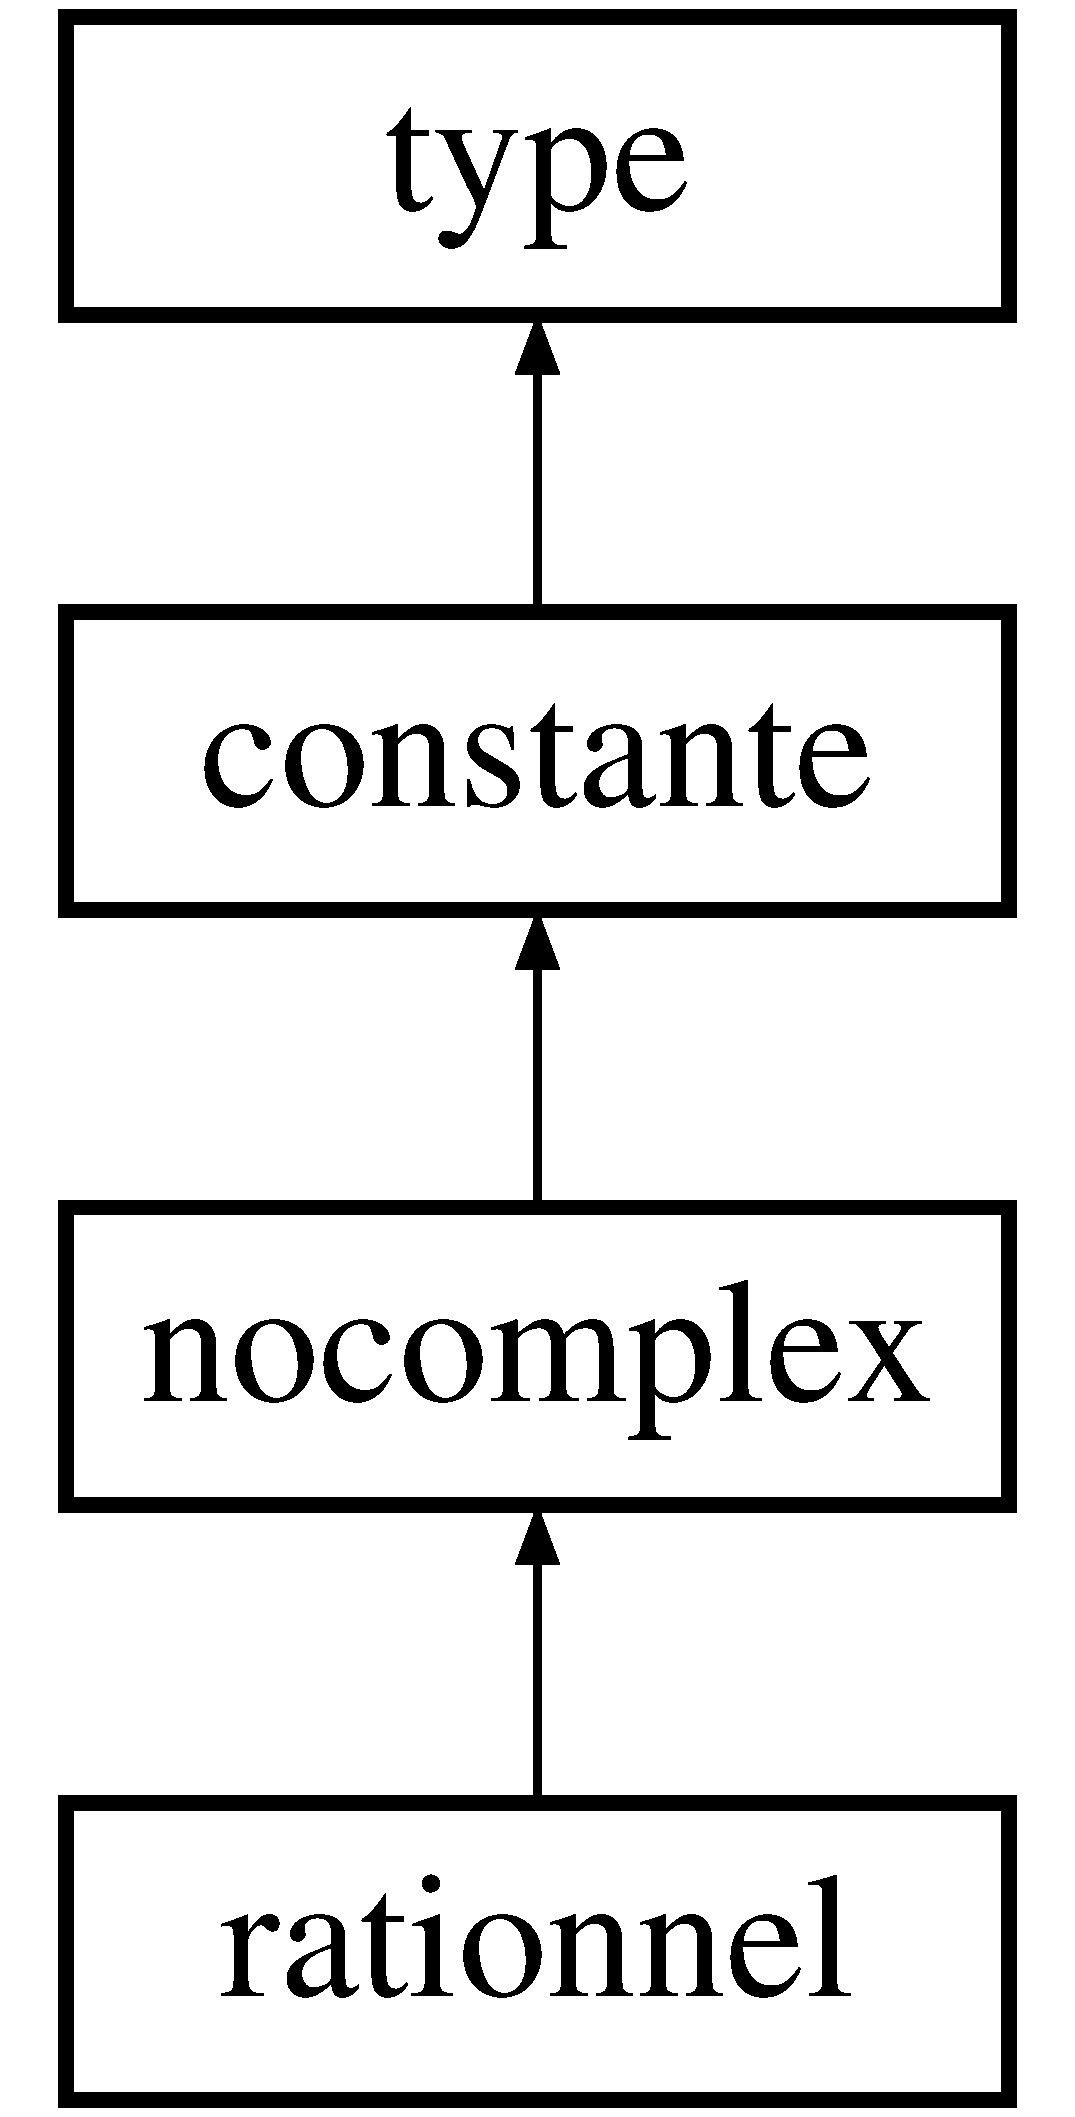
\includegraphics[height=4.000000cm]{classrationnel}
\end{center}
\end{figure}
\subsection*{Public Member Functions}
\begin{DoxyCompactItemize}
\item 
\hyperlink{classrationnel_a92b822d1a85e77456f9db2d0c691d74e}{rationnel} (int \-\_\-num=0, int \-\_\-denum=1)
\begin{DoxyCompactList}\small\item\em Constructeur. \end{DoxyCompactList}\item 
\hyperlink{classrationnel_a7411453ee0e517a0008e563938033750}{rationnel} (const Q\-String \&s)
\begin{DoxyCompactList}\small\item\em Constructeur. \end{DoxyCompactList}\item 
\hyperlink{classtype}{type} $\ast$ \hyperlink{classrationnel_a14d9d411058e146e075ccf16997e525e}{operator+} (\hyperlink{classtype}{type} \&t)
\begin{DoxyCompactList}\small\item\em Operateur +. \end{DoxyCompactList}\item 
\hyperlink{classtype}{type} $\ast$ \hyperlink{classrationnel_ae36b04407cc70d425ed0292975b0d1e9}{operator/} (\hyperlink{classtype}{type} \&t)
\begin{DoxyCompactList}\small\item\em Operateur /. \end{DoxyCompactList}\item 
\hyperlink{classtype}{type} $\ast$ \hyperlink{classrationnel_a49250cb9001aad230e5193515ee74efa}{operator$\ast$} (\hyperlink{classtype}{type} \&t)
\begin{DoxyCompactList}\small\item\em Operateur $\ast$. \end{DoxyCompactList}\item 
\hyperlink{classtype}{type} $\ast$ \hyperlink{classrationnel_a3bdf6de1a2526ddafbf1831a9af11dc9}{operator-\/} (\hyperlink{classtype}{type} \&t)
\begin{DoxyCompactList}\small\item\em Operateur -\/. \end{DoxyCompactList}\item 
\hyperlink{classtype}{type} $\ast$ \hyperlink{classrationnel_ad34af896f760a0271286e2dbbf55ad9f}{sinus} (bool degre)
\begin{DoxyCompactList}\small\item\em Sinus. \end{DoxyCompactList}\item 
\hyperlink{classtype}{type} $\ast$ \hyperlink{classrationnel_afd9fd9a30f034952ce889d46a07de617}{pow} (\hyperlink{classtype}{type} \&t)
\begin{DoxyCompactList}\small\item\em Pow. \end{DoxyCompactList}\item 
\hyperlink{classtype}{type} $\ast$ \hyperlink{classrationnel_aa73709167be428fafc4d95a31f4c3cc0}{sign} ()
\begin{DoxyCompactList}\small\item\em sign \end{DoxyCompactList}\item 
\hyperlink{classtype}{type} $\ast$ \hyperlink{classrationnel_a4a2f7528592b31a367799a79c336395c}{cosinus} (bool degre)
\begin{DoxyCompactList}\small\item\em Cosinus. \end{DoxyCompactList}\item 
\hyperlink{classtype}{type} $\ast$ \hyperlink{classrationnel_ac2bdc47a11ea3d010f006256f6e14f79}{tangente} (bool degre)
\begin{DoxyCompactList}\small\item\em Tangente. \end{DoxyCompactList}\item 
\hyperlink{classtype}{type} $\ast$ \hyperlink{classrationnel_a107f6a0be55879bd49dd015144fdfde4}{sinush} (bool degre)
\begin{DoxyCompactList}\small\item\em Sinush. \end{DoxyCompactList}\item 
\hyperlink{classtype}{type} $\ast$ \hyperlink{classrationnel_af8de9bc6850dc5471d2e31ddf8e3866e}{cosinush} (bool degre)
\begin{DoxyCompactList}\small\item\em Cosinush. \end{DoxyCompactList}\item 
\hyperlink{classtype}{type} $\ast$ \hyperlink{classrationnel_a56135a99618c1fec82901c5e7f64a4a2}{tangenteh} (bool degre)
\begin{DoxyCompactList}\small\item\em Tangenteh. \end{DoxyCompactList}\item 
\hyperlink{classtype}{type} $\ast$ \hyperlink{classrationnel_a59b1b593905de8676db02d5d2a5554c3}{ln} ()
\begin{DoxyCompactList}\small\item\em Ln. \end{DoxyCompactList}\item 
\hyperlink{classtype}{type} $\ast$ \hyperlink{classrationnel_a6bed14bda0b8546528454e7b2030645d}{log} ()
\begin{DoxyCompactList}\small\item\em Log. \end{DoxyCompactList}\item 
\hyperlink{classtype}{type} $\ast$ \hyperlink{classrationnel_a75336cd670c61195c833f8459c02c3b5}{inv} ()
\begin{DoxyCompactList}\small\item\em Inv. \end{DoxyCompactList}\item 
\hyperlink{classtype}{type} $\ast$ \hyperlink{classrationnel_ad37ab4380b5ff66104748ecc0bf5babe}{sqrt} ()
\begin{DoxyCompactList}\small\item\em Sqrt. \end{DoxyCompactList}\item 
\hyperlink{classtype}{type} $\ast$ \hyperlink{classrationnel_ab9f341fd09499253dd1f9b6f15795576}{sqr} ()
\begin{DoxyCompactList}\small\item\em Sqr. \end{DoxyCompactList}\item 
\hyperlink{classtype}{type} $\ast$ \hyperlink{classrationnel_a9bca6086c4a5083765d87324418a86ab}{cube} ()
\begin{DoxyCompactList}\small\item\em Cube. \end{DoxyCompactList}\item 
Q\-String \hyperlink{classrationnel_a6c905c688ae54647074a5ddf3ef648bd}{to\-Q\-String} ()
\begin{DoxyCompactList}\small\item\em to\-Q\-String \end{DoxyCompactList}\item 
Q\-String \hyperlink{classrationnel_a1418b1d6ac37f7948affefa7b8d0f314}{eval} ()
\begin{DoxyCompactList}\small\item\em eval \end{DoxyCompactList}\item 
void \hyperlink{classrationnel_a236e82f84556d0fcd978164529f9bf67}{simplifie} ()
\begin{DoxyCompactList}\small\item\em simplifie \end{DoxyCompactList}\item 
int \hyperlink{classrationnel_a7e10c925a450321f53a50636177561e5}{pgcd} (int, int) const 
\begin{DoxyCompactList}\small\item\em pgcd \end{DoxyCompactList}\item 
int \hyperlink{classrationnel_a9c4167d0aafd3bf9460ae58a81a0d29f}{get\-Num} ()
\begin{DoxyCompactList}\small\item\em get\-Num \end{DoxyCompactList}\item 
int \hyperlink{classrationnel_abb14c1aafb5b4e8f28d5c770e2e1523e}{get\-Denum} ()
\begin{DoxyCompactList}\small\item\em get\-Denum \end{DoxyCompactList}\end{DoxyCompactItemize}


\subsection{Detailed Description}
Classe representant une fraction. 

Derive de nocomplex 

\subsection{Constructor \& Destructor Documentation}
\hypertarget{classrationnel_a92b822d1a85e77456f9db2d0c691d74e}{\index{rationnel@{rationnel}!rationnel@{rationnel}}
\index{rationnel@{rationnel}!rationnel@{rationnel}}
\subsubsection[{rationnel}]{\setlength{\rightskip}{0pt plus 5cm}rationnel\-::rationnel (
\begin{DoxyParamCaption}
\item[{int}]{\-\_\-num = {\ttfamily 0}, }
\item[{int}]{\-\_\-denum = {\ttfamily 1}}
\end{DoxyParamCaption}
)\hspace{0.3cm}{\ttfamily [inline]}}}\label{classrationnel_a92b822d1a85e77456f9db2d0c691d74e}


Constructeur. 

Construit une fraction a partir de deux entiers \-: numerateur et denominateur \hypertarget{classrationnel_a7411453ee0e517a0008e563938033750}{\index{rationnel@{rationnel}!rationnel@{rationnel}}
\index{rationnel@{rationnel}!rationnel@{rationnel}}
\subsubsection[{rationnel}]{\setlength{\rightskip}{0pt plus 5cm}rationnel\-::rationnel (
\begin{DoxyParamCaption}
\item[{const Q\-String \&}]{s}
\end{DoxyParamCaption}
)\hspace{0.3cm}{\ttfamily [inline]}}}\label{classrationnel_a7411453ee0e517a0008e563938033750}


Constructeur. 

Construit une fraction a partir d'une Q\-String 

\subsection{Member Function Documentation}
\hypertarget{classrationnel_a4a2f7528592b31a367799a79c336395c}{\index{rationnel@{rationnel}!cosinus@{cosinus}}
\index{cosinus@{cosinus}!rationnel@{rationnel}}
\subsubsection[{cosinus}]{\setlength{\rightskip}{0pt plus 5cm}{\bf type} $\ast$ rationnel\-::cosinus (
\begin{DoxyParamCaption}
\item[{bool}]{degre}
\end{DoxyParamCaption}
)\hspace{0.3cm}{\ttfamily [virtual]}}}\label{classrationnel_a4a2f7528592b31a367799a79c336395c}


Cosinus. 

Implementation de l'operateur unaire cosinus (methode virtuelle dans la classe mere) \begin{DoxyReturn}{Returns}
Pointeur sur type, resultat de l'operation 
\end{DoxyReturn}


Implements \hyperlink{classnocomplex_a2c3aa4791fe0c123079b0332a5978939}{nocomplex}.

\hypertarget{classrationnel_af8de9bc6850dc5471d2e31ddf8e3866e}{\index{rationnel@{rationnel}!cosinush@{cosinush}}
\index{cosinush@{cosinush}!rationnel@{rationnel}}
\subsubsection[{cosinush}]{\setlength{\rightskip}{0pt plus 5cm}{\bf type} $\ast$ rationnel\-::cosinush (
\begin{DoxyParamCaption}
\item[{bool}]{degre}
\end{DoxyParamCaption}
)\hspace{0.3cm}{\ttfamily [virtual]}}}\label{classrationnel_af8de9bc6850dc5471d2e31ddf8e3866e}


Cosinush. 

Implementation de l'operateur unaire cosinush (methode virtuelle dans la classe mere) \begin{DoxyReturn}{Returns}
Pointeur sur type, resultat de l'operation 
\end{DoxyReturn}


Implements \hyperlink{classnocomplex_ae92516f1c7c78298a11e8e34355b9f81}{nocomplex}.

\hypertarget{classrationnel_a9bca6086c4a5083765d87324418a86ab}{\index{rationnel@{rationnel}!cube@{cube}}
\index{cube@{cube}!rationnel@{rationnel}}
\subsubsection[{cube}]{\setlength{\rightskip}{0pt plus 5cm}{\bf type} $\ast$ rationnel\-::cube (
\begin{DoxyParamCaption}
{}
\end{DoxyParamCaption}
)\hspace{0.3cm}{\ttfamily [virtual]}}}\label{classrationnel_a9bca6086c4a5083765d87324418a86ab}


Cube. 

Implementation de l'operateur unaire Cube (methode virtuelle dans la classe mere) \begin{DoxyReturn}{Returns}
Pointeur sur type, resultat de l'operation 
\end{DoxyReturn}


Implements \hyperlink{classnocomplex_ad84e4a7a269024da4551a8e99078e41d}{nocomplex}.

\hypertarget{classrationnel_a1418b1d6ac37f7948affefa7b8d0f314}{\index{rationnel@{rationnel}!eval@{eval}}
\index{eval@{eval}!rationnel@{rationnel}}
\subsubsection[{eval}]{\setlength{\rightskip}{0pt plus 5cm}Q\-String rationnel\-::eval (
\begin{DoxyParamCaption}
{}
\end{DoxyParamCaption}
)\hspace{0.3cm}{\ttfamily [virtual]}}}\label{classrationnel_a1418b1d6ac37f7948affefa7b8d0f314}


eval 

Implementation de l'operateur unaire eval (methode virtuelle dans la classe mere) Permet d'arrondir une fraction 
\begin{DoxyParams}{Parameters}
{\em t} & \-: Pointeur sur un type \\
\hline
\end{DoxyParams}
\begin{DoxyReturn}{Returns}
Pointeur sur type, resultat de l'operation 
\end{DoxyReturn}


Reimplemented from \hyperlink{classnocomplex_a8831dff2cd793c03618b6e0751ffc026}{nocomplex}.

\hypertarget{classrationnel_abb14c1aafb5b4e8f28d5c770e2e1523e}{\index{rationnel@{rationnel}!get\-Denum@{get\-Denum}}
\index{get\-Denum@{get\-Denum}!rationnel@{rationnel}}
\subsubsection[{get\-Denum}]{\setlength{\rightskip}{0pt plus 5cm}int rationnel\-::get\-Denum (
\begin{DoxyParamCaption}
{}
\end{DoxyParamCaption}
)\hspace{0.3cm}{\ttfamily [inline]}}}\label{classrationnel_abb14c1aafb5b4e8f28d5c770e2e1523e}


get\-Denum 

Accesseur du denominateur \begin{DoxyReturn}{Returns}
denominateur(entier) 
\end{DoxyReturn}
\hypertarget{classrationnel_a9c4167d0aafd3bf9460ae58a81a0d29f}{\index{rationnel@{rationnel}!get\-Num@{get\-Num}}
\index{get\-Num@{get\-Num}!rationnel@{rationnel}}
\subsubsection[{get\-Num}]{\setlength{\rightskip}{0pt plus 5cm}int rationnel\-::get\-Num (
\begin{DoxyParamCaption}
{}
\end{DoxyParamCaption}
)\hspace{0.3cm}{\ttfamily [inline]}}}\label{classrationnel_a9c4167d0aafd3bf9460ae58a81a0d29f}


get\-Num 

Accesseur du numerateur \begin{DoxyReturn}{Returns}
numerateur(entier) 
\end{DoxyReturn}
\hypertarget{classrationnel_a75336cd670c61195c833f8459c02c3b5}{\index{rationnel@{rationnel}!inv@{inv}}
\index{inv@{inv}!rationnel@{rationnel}}
\subsubsection[{inv}]{\setlength{\rightskip}{0pt plus 5cm}{\bf type} $\ast$ rationnel\-::inv (
\begin{DoxyParamCaption}
{}
\end{DoxyParamCaption}
)\hspace{0.3cm}{\ttfamily [virtual]}}}\label{classrationnel_a75336cd670c61195c833f8459c02c3b5}


Inv. 

Implementation de l'operateur unaire inv (methode virtuelle dans la classe mere) \begin{DoxyReturn}{Returns}
Pointeur sur type, resultat de l'operation 
\end{DoxyReturn}


Implements \hyperlink{classnocomplex_a9e0f97f51c50b11022c6d0b409c26ecf}{nocomplex}.

\hypertarget{classrationnel_a59b1b593905de8676db02d5d2a5554c3}{\index{rationnel@{rationnel}!ln@{ln}}
\index{ln@{ln}!rationnel@{rationnel}}
\subsubsection[{ln}]{\setlength{\rightskip}{0pt plus 5cm}{\bf type} $\ast$ rationnel\-::ln (
\begin{DoxyParamCaption}
{}
\end{DoxyParamCaption}
)\hspace{0.3cm}{\ttfamily [virtual]}}}\label{classrationnel_a59b1b593905de8676db02d5d2a5554c3}


Ln. 

Implementation de l'operateur unaire ln (methode virtuelle dans la classe mere) \begin{DoxyReturn}{Returns}
Pointeur sur type, resultat de l'operation 
\end{DoxyReturn}


Implements \hyperlink{classnocomplex_ab3e91b96595fef9d53a5cfb93291c8f0}{nocomplex}.

\hypertarget{classrationnel_a6bed14bda0b8546528454e7b2030645d}{\index{rationnel@{rationnel}!log@{log}}
\index{log@{log}!rationnel@{rationnel}}
\subsubsection[{log}]{\setlength{\rightskip}{0pt plus 5cm}{\bf type} $\ast$ rationnel\-::log (
\begin{DoxyParamCaption}
{}
\end{DoxyParamCaption}
)\hspace{0.3cm}{\ttfamily [virtual]}}}\label{classrationnel_a6bed14bda0b8546528454e7b2030645d}


Log. 

Implementation de l'operateur unaire log (methode virtuelle dans la classe mere) \begin{DoxyReturn}{Returns}
Pointeur sur type, resultat de l'operation 
\end{DoxyReturn}


Implements \hyperlink{classnocomplex_a0f7a5802123786d1461271d5c05158ca}{nocomplex}.

\hypertarget{classrationnel_a49250cb9001aad230e5193515ee74efa}{\index{rationnel@{rationnel}!operator$\ast$@{operator$\ast$}}
\index{operator$\ast$@{operator$\ast$}!rationnel@{rationnel}}
\subsubsection[{operator$\ast$}]{\setlength{\rightskip}{0pt plus 5cm}{\bf type} $\ast$ rationnel\-::operator$\ast$ (
\begin{DoxyParamCaption}
\item[{{\bf type} \&}]{t}
\end{DoxyParamCaption}
)\hspace{0.3cm}{\ttfamily [virtual]}}}\label{classrationnel_a49250cb9001aad230e5193515ee74efa}


Operateur $\ast$. 

Implementation de l'operateur binaire $\ast$ (methode virtuelle dans la classe mere) 
\begin{DoxyParams}{Parameters}
{\em t} & \-: Pointeur sur un type \\
\hline
\end{DoxyParams}
\begin{DoxyReturn}{Returns}
Pointeur sur type, resultat de l'operation 
\end{DoxyReturn}


Implements \hyperlink{classnocomplex_ac84954cbe0bd9c77eab88c0b97b34c2b}{nocomplex}.

\hypertarget{classrationnel_a14d9d411058e146e075ccf16997e525e}{\index{rationnel@{rationnel}!operator+@{operator+}}
\index{operator+@{operator+}!rationnel@{rationnel}}
\subsubsection[{operator+}]{\setlength{\rightskip}{0pt plus 5cm}{\bf type} $\ast$ rationnel\-::operator+ (
\begin{DoxyParamCaption}
\item[{{\bf type} \&}]{t}
\end{DoxyParamCaption}
)\hspace{0.3cm}{\ttfamily [virtual]}}}\label{classrationnel_a14d9d411058e146e075ccf16997e525e}


Operateur +. 

Implementation de l'operateur binaire + (methode virtuelle dans la classe mere) 
\begin{DoxyParams}{Parameters}
{\em t} & \-: Pointeur sur un type \\
\hline
\end{DoxyParams}
\begin{DoxyReturn}{Returns}
Pointeur sur type, resultat de l'operation 
\end{DoxyReturn}


Implements \hyperlink{classnocomplex_af3d04b00f4f82d3a35cad0ca023093f4}{nocomplex}.

\hypertarget{classrationnel_a3bdf6de1a2526ddafbf1831a9af11dc9}{\index{rationnel@{rationnel}!operator-\/@{operator-\/}}
\index{operator-\/@{operator-\/}!rationnel@{rationnel}}
\subsubsection[{operator-\/}]{\setlength{\rightskip}{0pt plus 5cm}{\bf type} $\ast$ rationnel\-::operator-\/ (
\begin{DoxyParamCaption}
\item[{{\bf type} \&}]{t}
\end{DoxyParamCaption}
)\hspace{0.3cm}{\ttfamily [virtual]}}}\label{classrationnel_a3bdf6de1a2526ddafbf1831a9af11dc9}


Operateur -\/. 

Implementation de l'operateur binaire -\/ (methode virtuelle dans la classe mere) 
\begin{DoxyParams}{Parameters}
{\em t} & \-: Pointeur sur un type \\
\hline
\end{DoxyParams}
\begin{DoxyReturn}{Returns}
Pointeur sur type, resultat de l'operation 
\end{DoxyReturn}


Implements \hyperlink{classnocomplex_a2005c3a0fcaa1f360561539931ffc578}{nocomplex}.

\hypertarget{classrationnel_ae36b04407cc70d425ed0292975b0d1e9}{\index{rationnel@{rationnel}!operator/@{operator/}}
\index{operator/@{operator/}!rationnel@{rationnel}}
\subsubsection[{operator/}]{\setlength{\rightskip}{0pt plus 5cm}{\bf type} $\ast$ rationnel\-::operator/ (
\begin{DoxyParamCaption}
\item[{{\bf type} \&}]{t}
\end{DoxyParamCaption}
)\hspace{0.3cm}{\ttfamily [virtual]}}}\label{classrationnel_ae36b04407cc70d425ed0292975b0d1e9}


Operateur /. 

Implementation de l'operateur binaire / (methode virtuelle dans la classe mere) 
\begin{DoxyParams}{Parameters}
{\em t} & \-: Pointeur sur un type \\
\hline
\end{DoxyParams}
\begin{DoxyReturn}{Returns}
Pointeur sur type, resultat de l'operation 
\end{DoxyReturn}


Implements \hyperlink{classnocomplex_a47942bdcc78cfc5d5e867c9f9836a465}{nocomplex}.

\hypertarget{classrationnel_a7e10c925a450321f53a50636177561e5}{\index{rationnel@{rationnel}!pgcd@{pgcd}}
\index{pgcd@{pgcd}!rationnel@{rationnel}}
\subsubsection[{pgcd}]{\setlength{\rightskip}{0pt plus 5cm}int rationnel\-::pgcd (
\begin{DoxyParamCaption}
\item[{int}]{a, }
\item[{int}]{b}
\end{DoxyParamCaption}
) const}}\label{classrationnel_a7e10c925a450321f53a50636177561e5}


pgcd 

Calcul le pgcd de deux entier 
\begin{DoxyParams}{Parameters}
{\em 2} & entiers \\
\hline
\end{DoxyParams}
\hypertarget{classrationnel_afd9fd9a30f034952ce889d46a07de617}{\index{rationnel@{rationnel}!pow@{pow}}
\index{pow@{pow}!rationnel@{rationnel}}
\subsubsection[{pow}]{\setlength{\rightskip}{0pt plus 5cm}{\bf type} $\ast$ rationnel\-::pow (
\begin{DoxyParamCaption}
\item[{{\bf type} \&}]{t}
\end{DoxyParamCaption}
)\hspace{0.3cm}{\ttfamily [virtual]}}}\label{classrationnel_afd9fd9a30f034952ce889d46a07de617}


Pow. 

Implementation de l'operateur binaire pow (methode virtuelle dans la classe mere) 
\begin{DoxyParams}{Parameters}
{\em t} & \-: Pointeur sur un type \\
\hline
\end{DoxyParams}
\begin{DoxyReturn}{Returns}
Pointeur sur type, resultat de l'operation 
\end{DoxyReturn}


Implements \hyperlink{classnocomplex_a1ad1b692783c8449efb03cc0dc5d1f3c}{nocomplex}.

\hypertarget{classrationnel_aa73709167be428fafc4d95a31f4c3cc0}{\index{rationnel@{rationnel}!sign@{sign}}
\index{sign@{sign}!rationnel@{rationnel}}
\subsubsection[{sign}]{\setlength{\rightskip}{0pt plus 5cm}{\bf type} $\ast$ rationnel\-::sign (
\begin{DoxyParamCaption}
{}
\end{DoxyParamCaption}
)\hspace{0.3cm}{\ttfamily [virtual]}}}\label{classrationnel_aa73709167be428fafc4d95a31f4c3cc0}


sign 

Implementation de l'operateur unaire sign (methode virtuelle dans la classe mere) Inverse le signe de la constante 
\begin{DoxyParams}{Parameters}
{\em t} & \-: Pointeur sur un type \\
\hline
\end{DoxyParams}
\begin{DoxyReturn}{Returns}
Pointeur sur type, resultat de l'operation 
\end{DoxyReturn}


Implements \hyperlink{classnocomplex_acd1c0365d1a2ed160934320cff01cecd}{nocomplex}.

\hypertarget{classrationnel_a236e82f84556d0fcd978164529f9bf67}{\index{rationnel@{rationnel}!simplifie@{simplifie}}
\index{simplifie@{simplifie}!rationnel@{rationnel}}
\subsubsection[{simplifie}]{\setlength{\rightskip}{0pt plus 5cm}void rationnel\-::simplifie (
\begin{DoxyParamCaption}
{}
\end{DoxyParamCaption}
)}}\label{classrationnel_a236e82f84556d0fcd978164529f9bf67}


simplifie 

Simplifie la fration. Utilisation du P\-G\-C\-D \hypertarget{classrationnel_ad34af896f760a0271286e2dbbf55ad9f}{\index{rationnel@{rationnel}!sinus@{sinus}}
\index{sinus@{sinus}!rationnel@{rationnel}}
\subsubsection[{sinus}]{\setlength{\rightskip}{0pt plus 5cm}{\bf type} $\ast$ rationnel\-::sinus (
\begin{DoxyParamCaption}
\item[{bool}]{degre}
\end{DoxyParamCaption}
)\hspace{0.3cm}{\ttfamily [virtual]}}}\label{classrationnel_ad34af896f760a0271286e2dbbf55ad9f}


Sinus. 

Implementation de l'operateur unaire sinus (methode virtuelle dans la classe mere) 
\begin{DoxyParams}{Parameters}
{\em t} & \-: Pointeur sur un type \\
\hline
\end{DoxyParams}
\begin{DoxyReturn}{Returns}
Pointeur sur type, resultat de l'operation 
\end{DoxyReturn}


Implements \hyperlink{classnocomplex_aea2ba416f34c37ad2cf751b6220d53b8}{nocomplex}.

\hypertarget{classrationnel_a107f6a0be55879bd49dd015144fdfde4}{\index{rationnel@{rationnel}!sinush@{sinush}}
\index{sinush@{sinush}!rationnel@{rationnel}}
\subsubsection[{sinush}]{\setlength{\rightskip}{0pt plus 5cm}{\bf type} $\ast$ rationnel\-::sinush (
\begin{DoxyParamCaption}
\item[{bool}]{degre}
\end{DoxyParamCaption}
)\hspace{0.3cm}{\ttfamily [virtual]}}}\label{classrationnel_a107f6a0be55879bd49dd015144fdfde4}


Sinush. 

Implementation de l'operateur unaire sinush (methode virtuelle dans la classe mere) \begin{DoxyReturn}{Returns}
Pointeur sur type, resultat de l'operation 
\end{DoxyReturn}


Implements \hyperlink{classnocomplex_a4df698a9ee147b77aaab9f63840b1012}{nocomplex}.

\hypertarget{classrationnel_ab9f341fd09499253dd1f9b6f15795576}{\index{rationnel@{rationnel}!sqr@{sqr}}
\index{sqr@{sqr}!rationnel@{rationnel}}
\subsubsection[{sqr}]{\setlength{\rightskip}{0pt plus 5cm}{\bf type} $\ast$ rationnel\-::sqr (
\begin{DoxyParamCaption}
{}
\end{DoxyParamCaption}
)\hspace{0.3cm}{\ttfamily [virtual]}}}\label{classrationnel_ab9f341fd09499253dd1f9b6f15795576}


Sqr. 

Implementation de l'operateur unaire sqr (methode virtuelle dans la classe mere) \begin{DoxyReturn}{Returns}
Pointeur sur type, resultat de l'operation 
\end{DoxyReturn}


Implements \hyperlink{classnocomplex_a5665f2bcf5ad839e92c31f38f3dfc7b7}{nocomplex}.

\hypertarget{classrationnel_ad37ab4380b5ff66104748ecc0bf5babe}{\index{rationnel@{rationnel}!sqrt@{sqrt}}
\index{sqrt@{sqrt}!rationnel@{rationnel}}
\subsubsection[{sqrt}]{\setlength{\rightskip}{0pt plus 5cm}{\bf type} $\ast$ rationnel\-::sqrt (
\begin{DoxyParamCaption}
{}
\end{DoxyParamCaption}
)\hspace{0.3cm}{\ttfamily [virtual]}}}\label{classrationnel_ad37ab4380b5ff66104748ecc0bf5babe}


Sqrt. 

Implementation de l'operateur unaire sqrt (methode virtuelle dans la classe mere) 
\begin{DoxyParams}{Parameters}
{\em t} & \-: Pointeur sur un type \\
\hline
\end{DoxyParams}
\begin{DoxyReturn}{Returns}
Pointeur sur type, resultat de l'operation 
\end{DoxyReturn}


Implements \hyperlink{classnocomplex_a7f693a0869814705bcc3b8add799e6cd}{nocomplex}.

\hypertarget{classrationnel_ac2bdc47a11ea3d010f006256f6e14f79}{\index{rationnel@{rationnel}!tangente@{tangente}}
\index{tangente@{tangente}!rationnel@{rationnel}}
\subsubsection[{tangente}]{\setlength{\rightskip}{0pt plus 5cm}{\bf type} $\ast$ rationnel\-::tangente (
\begin{DoxyParamCaption}
\item[{bool}]{degre}
\end{DoxyParamCaption}
)\hspace{0.3cm}{\ttfamily [virtual]}}}\label{classrationnel_ac2bdc47a11ea3d010f006256f6e14f79}


Tangente. 

Implementation de l'operateur unaire tangente (methode virtuelle dans la classe mere) \begin{DoxyReturn}{Returns}
Pointeur sur type, resultat de l'operation 
\end{DoxyReturn}


Implements \hyperlink{classnocomplex_a2e7f4563e7d602c79e356dcb5472e341}{nocomplex}.

\hypertarget{classrationnel_a56135a99618c1fec82901c5e7f64a4a2}{\index{rationnel@{rationnel}!tangenteh@{tangenteh}}
\index{tangenteh@{tangenteh}!rationnel@{rationnel}}
\subsubsection[{tangenteh}]{\setlength{\rightskip}{0pt plus 5cm}{\bf type} $\ast$ rationnel\-::tangenteh (
\begin{DoxyParamCaption}
\item[{bool}]{degre}
\end{DoxyParamCaption}
)\hspace{0.3cm}{\ttfamily [virtual]}}}\label{classrationnel_a56135a99618c1fec82901c5e7f64a4a2}


Tangenteh. 

Implementation de l'operateur unaire tangenteh (methode virtuelle dans la classe mere) \begin{DoxyReturn}{Returns}
Pointeur sur type, resultat de l'operation 
\end{DoxyReturn}


Implements \hyperlink{classnocomplex_a79aa6c234a5a66bfe18c39794e56c277}{nocomplex}.

\hypertarget{classrationnel_a6c905c688ae54647074a5ddf3ef648bd}{\index{rationnel@{rationnel}!to\-Q\-String@{to\-Q\-String}}
\index{to\-Q\-String@{to\-Q\-String}!rationnel@{rationnel}}
\subsubsection[{to\-Q\-String}]{\setlength{\rightskip}{0pt plus 5cm}Q\-String rationnel\-::to\-Q\-String (
\begin{DoxyParamCaption}
{}
\end{DoxyParamCaption}
)\hspace{0.3cm}{\ttfamily [virtual]}}}\label{classrationnel_a6c905c688ae54647074a5ddf3ef648bd}


to\-Q\-String 

Transforme l'objet Qstring. Permet ensuite l'affichage dans des widget \begin{DoxyReturn}{Returns}
Qstring \-: chaine resultat 
\end{DoxyReturn}


Implements \hyperlink{classtype_ab61f01d56f3896cc99788a1a18c4b0c2}{type}.



The documentation for this class was generated from the following files\-:\begin{DoxyCompactItemize}
\item 
Code/projet\-\_\-lo21/\hyperlink{rationnel_8h}{rationnel.\-h}\item 
Code/projet\-\_\-lo21/rationnel.\-cpp\end{DoxyCompactItemize}

\hypertarget{classreel}{\section{reel Class Reference}
\label{classreel}\index{reel@{reel}}
}


{\ttfamily \#include $<$reel.\-h$>$}



Inherits \hyperlink{classnocomplex}{nocomplex}.

\subsection*{Public Member Functions}
\begin{DoxyCompactItemize}
\item 
\hyperlink{classreel_af400a93dfd7cfa7447f8751ab32c48fc}{reel} (double val=0)
\item 
\hyperlink{classreel_a6399912ce32c14c918ce5b6fb0b294dc}{reel} (const Q\-String \&s)
\item 
double \hyperlink{classreel_ad1d16e6ce54fc6b8844757a8f04300ca}{get\-Data} ()
\item 
\hyperlink{classtype}{type} $\ast$ \hyperlink{classreel_af2ae884e68ab28b286cf9940f05f59d9}{operator+} (\hyperlink{classtype}{type} \&t)
\begin{DoxyCompactList}\small\item\em Operateur +. \end{DoxyCompactList}\item 
\hyperlink{classtype}{type} $\ast$ \hyperlink{classreel_a3bc55f29b377547040d47be018b73fe6}{operator/} (\hyperlink{classtype}{type} \&t)
\begin{DoxyCompactList}\small\item\em Operateur /. \end{DoxyCompactList}\item 
\hyperlink{classtype}{type} $\ast$ \hyperlink{classreel_a044791a71fd9926cbedf3f19f6eea122}{operator$\ast$} (\hyperlink{classtype}{type} \&t)
\begin{DoxyCompactList}\small\item\em Operateur $\ast$. \end{DoxyCompactList}\item 
\hyperlink{classtype}{type} $\ast$ \hyperlink{classreel_a9cd96b762004392eda5216262201322c}{operator-\/} (\hyperlink{classtype}{type} \&t)
\begin{DoxyCompactList}\small\item\em Operateur -\/. \end{DoxyCompactList}\item 
\hyperlink{classtype}{type} $\ast$ \hyperlink{classreel_a8436fd89eda982a6b023e2f7081b5cb0}{sinus} ()
\begin{DoxyCompactList}\small\item\em Sinus. \end{DoxyCompactList}\item 
\hyperlink{classtype}{type} $\ast$ \hyperlink{classreel_a4fdea6a69bd78b2593fb44cc172fc7bf}{pow} (\hyperlink{classtype}{type} \&t)
\item 
\hyperlink{classtype}{type} $\ast$ \hyperlink{classreel_a7bf66e936c424f243a534406dbe8e8d7}{mod} (\hyperlink{classtype}{type} \&t)
\item 
\hyperlink{classtype}{type} $\ast$ \hyperlink{classreel_a9a172c44e0a496059bdd1c4d53a98590}{sign} ()
\item 
\hyperlink{classtype}{type} $\ast$ \hyperlink{classreel_a4d1fb90011705658295e922d525a91dd}{cosinus} ()
\begin{DoxyCompactList}\small\item\em Cosinus. \end{DoxyCompactList}\item 
\hyperlink{classtype}{type} $\ast$ \hyperlink{classreel_a8ded2c9525ab4937f20b28d31a381442}{tangente} ()
\begin{DoxyCompactList}\small\item\em Tangente. \end{DoxyCompactList}\item 
\hyperlink{classtype}{type} $\ast$ \hyperlink{classreel_ad404481ff6381767546b93ca0c4ba3e3}{sinush} ()
\begin{DoxyCompactList}\small\item\em Sinush. \end{DoxyCompactList}\item 
\hyperlink{classtype}{type} $\ast$ \hyperlink{classreel_ad2d6ed0dcaa8fa7b410ca1a84c0d3f57}{cosinush} ()
\begin{DoxyCompactList}\small\item\em Cosinush. \end{DoxyCompactList}\item 
\hyperlink{classtype}{type} $\ast$ \hyperlink{classreel_a4d66c94b0c33019d0dfae8deb2bb41a3}{tangenteh} ()
\begin{DoxyCompactList}\small\item\em Tangenteh. \end{DoxyCompactList}\item 
\hyperlink{classtype}{type} $\ast$ \hyperlink{classreel_a5d09de0b7e0856eb63d333f766c770ed}{ln} ()
\begin{DoxyCompactList}\small\item\em Ln. \end{DoxyCompactList}\item 
\hyperlink{classtype}{type} $\ast$ \hyperlink{classreel_adcf600e2052329def8e10e81e35ef96e}{log} ()
\begin{DoxyCompactList}\small\item\em Log. \end{DoxyCompactList}\item 
\hyperlink{classtype}{type} $\ast$ \hyperlink{classreel_ab863c6b28a5345dbf7657b4b5121c2f7}{inv} ()
\begin{DoxyCompactList}\small\item\em Inv. \end{DoxyCompactList}\item 
\hyperlink{classtype}{type} $\ast$ \hyperlink{classreel_a980bc278bf5537519ee05746262ebb6a}{sqrt} ()
\begin{DoxyCompactList}\small\item\em Sqrt. \end{DoxyCompactList}\item 
\hyperlink{classtype}{type} $\ast$ \hyperlink{classreel_ad295586d5862f6dc41966f25c365c4a1}{sqr} ()
\begin{DoxyCompactList}\small\item\em Sqr. \end{DoxyCompactList}\item 
\hyperlink{classtype}{type} $\ast$ \hyperlink{classreel_a3a2dc28d66ee81177a986fca957f6fd5}{cube} ()
\begin{DoxyCompactList}\small\item\em Cube. \end{DoxyCompactList}\item 
\hyperlink{classtype}{type} $\ast$ \hyperlink{classreel_ac56ec7c9e6b96b85723e518e70ecfc24}{fact} ()
\begin{DoxyCompactList}\small\item\em Fact. \end{DoxyCompactList}\item 
\hyperlink{classtype}{type} $\ast$ \hyperlink{classreel_a5d0427a4f39bbb96411cb5a1a0320625}{eval} ()
\begin{DoxyCompactList}\small\item\em eval \end{DoxyCompactList}\item 
Q\-String \hyperlink{classreel_a6b06a283958b63fde5c12382b744a8c9}{to\-Q\-String} ()
\begin{DoxyCompactList}\small\item\em to\-Q\-String \end{DoxyCompactList}\end{DoxyCompactItemize}
\subsection*{Static Public Member Functions}
\begin{DoxyCompactItemize}
\item 
static bool \hyperlink{classreel_abdb4c9f0cd45c053b35f868885c5b822}{is\-Reel} (const Q\-String \&s)
\begin{DoxyCompactList}\small\item\em is\-Reel \end{DoxyCompactList}\end{DoxyCompactItemize}


\subsection{Constructor \& Destructor Documentation}
\hypertarget{classreel_af400a93dfd7cfa7447f8751ab32c48fc}{\index{reel@{reel}!reel@{reel}}
\index{reel@{reel}!reel@{reel}}
\subsubsection[{reel}]{\setlength{\rightskip}{0pt plus 5cm}reel\-::reel (
\begin{DoxyParamCaption}
\item[{double}]{val = {\ttfamily 0}}
\end{DoxyParamCaption}
)\hspace{0.3cm}{\ttfamily [inline]}}}\label{classreel_af400a93dfd7cfa7447f8751ab32c48fc}
\hypertarget{classreel_a6399912ce32c14c918ce5b6fb0b294dc}{\index{reel@{reel}!reel@{reel}}
\index{reel@{reel}!reel@{reel}}
\subsubsection[{reel}]{\setlength{\rightskip}{0pt plus 5cm}reel\-::reel (
\begin{DoxyParamCaption}
\item[{const Q\-String \&}]{s}
\end{DoxyParamCaption}
)\hspace{0.3cm}{\ttfamily [inline]}}}\label{classreel_a6399912ce32c14c918ce5b6fb0b294dc}


\subsection{Member Function Documentation}
\hypertarget{classreel_a4d1fb90011705658295e922d525a91dd}{\index{reel@{reel}!cosinus@{cosinus}}
\index{cosinus@{cosinus}!reel@{reel}}
\subsubsection[{cosinus}]{\setlength{\rightskip}{0pt plus 5cm}{\bf type} $\ast$ reel\-::cosinus (
\begin{DoxyParamCaption}
{}
\end{DoxyParamCaption}
)\hspace{0.3cm}{\ttfamily [virtual]}}}\label{classreel_a4d1fb90011705658295e922d525a91dd}


Cosinus. 

Implementation de l'operateur unaire cosinus (methode virtuelle pure dans la classe mere) \begin{DoxyReturn}{Returns}
Pointeur sur type, resultat de l'operation 
\end{DoxyReturn}


Implements \hyperlink{classtype_ac459ee75f7ab8d345c01a1f9a13f0728}{type}.

\hypertarget{classreel_ad2d6ed0dcaa8fa7b410ca1a84c0d3f57}{\index{reel@{reel}!cosinush@{cosinush}}
\index{cosinush@{cosinush}!reel@{reel}}
\subsubsection[{cosinush}]{\setlength{\rightskip}{0pt plus 5cm}{\bf type} $\ast$ reel\-::cosinush (
\begin{DoxyParamCaption}
{}
\end{DoxyParamCaption}
)\hspace{0.3cm}{\ttfamily [virtual]}}}\label{classreel_ad2d6ed0dcaa8fa7b410ca1a84c0d3f57}


Cosinush. 

Implementation de l'operateur unaire cosinush (methode virtuelle pure dans la classe mere) \begin{DoxyReturn}{Returns}
Pointeur sur type, resultat de l'operation 
\end{DoxyReturn}


Implements \hyperlink{classtype_acd7a105cccf58a42d6c09b40c91f75f0}{type}.

\hypertarget{classreel_a3a2dc28d66ee81177a986fca957f6fd5}{\index{reel@{reel}!cube@{cube}}
\index{cube@{cube}!reel@{reel}}
\subsubsection[{cube}]{\setlength{\rightskip}{0pt plus 5cm}{\bf type} $\ast$ reel\-::cube (
\begin{DoxyParamCaption}
{}
\end{DoxyParamCaption}
)\hspace{0.3cm}{\ttfamily [virtual]}}}\label{classreel_a3a2dc28d66ee81177a986fca957f6fd5}


Cube. 

Implementation de l'operateur unaire Cube (methode virtuelle pure dans la classe mere) \begin{DoxyReturn}{Returns}
Pointeur sur type, resultat de l'operation 
\end{DoxyReturn}


Implements \hyperlink{classtype_ae9ff7857936535092924b83aec1412c6}{type}.

\hypertarget{classreel_a5d0427a4f39bbb96411cb5a1a0320625}{\index{reel@{reel}!eval@{eval}}
\index{eval@{eval}!reel@{reel}}
\subsubsection[{eval}]{\setlength{\rightskip}{0pt plus 5cm}{\bf type}$\ast$ reel\-::eval (
\begin{DoxyParamCaption}
{}
\end{DoxyParamCaption}
)\hspace{0.3cm}{\ttfamily [inline]}, {\ttfamily [virtual]}}}\label{classreel_a5d0427a4f39bbb96411cb5a1a0320625}


eval 

Implementation de l'operateur unaire eval (methode virtuelle pure dans la classe mere) \begin{DoxyReturn}{Returns}
Pointeur sur type, resultat de l'operation 
\end{DoxyReturn}


Implements \hyperlink{classtype_a20555e9f6c76f728d94049bd72f65fc6}{type}.

\hypertarget{classreel_ac56ec7c9e6b96b85723e518e70ecfc24}{\index{reel@{reel}!fact@{fact}}
\index{fact@{fact}!reel@{reel}}
\subsubsection[{fact}]{\setlength{\rightskip}{0pt plus 5cm}{\bf type}$\ast$ reel\-::fact (
\begin{DoxyParamCaption}
{}
\end{DoxyParamCaption}
)\hspace{0.3cm}{\ttfamily [inline]}, {\ttfamily [virtual]}}}\label{classreel_ac56ec7c9e6b96b85723e518e70ecfc24}


Fact. 

Implementation de l'operateur unaire fact (methode virtuelle pure dans la classe mere) 
\begin{DoxyParams}{Parameters}
{\em t} & \-: Pointeur sur un type (Utilisation du polymorphisme) \\
\hline
\end{DoxyParams}
\begin{DoxyReturn}{Returns}
Pointeur sur type, resultat de l'operation 
\end{DoxyReturn}


Implements \hyperlink{classtype_aa5503ee1cdc7c88b058f9216e1e780c3}{type}.

\hypertarget{classreel_ad1d16e6ce54fc6b8844757a8f04300ca}{\index{reel@{reel}!get\-Data@{get\-Data}}
\index{get\-Data@{get\-Data}!reel@{reel}}
\subsubsection[{get\-Data}]{\setlength{\rightskip}{0pt plus 5cm}double reel\-::get\-Data (
\begin{DoxyParamCaption}
{}
\end{DoxyParamCaption}
)\hspace{0.3cm}{\ttfamily [inline]}}}\label{classreel_ad1d16e6ce54fc6b8844757a8f04300ca}
\hypertarget{classreel_ab863c6b28a5345dbf7657b4b5121c2f7}{\index{reel@{reel}!inv@{inv}}
\index{inv@{inv}!reel@{reel}}
\subsubsection[{inv}]{\setlength{\rightskip}{0pt plus 5cm}{\bf type} $\ast$ reel\-::inv (
\begin{DoxyParamCaption}
{}
\end{DoxyParamCaption}
)\hspace{0.3cm}{\ttfamily [virtual]}}}\label{classreel_ab863c6b28a5345dbf7657b4b5121c2f7}


Inv. 

Implementation de l'operateur unaire inv (methode virtuelle pure dans la classe mere) \begin{DoxyReturn}{Returns}
Pointeur sur type, resultat de l'operation 
\end{DoxyReturn}


Implements \hyperlink{classtype_a5eeb7c768cc90a0e9abd91d585169264}{type}.

\hypertarget{classreel_abdb4c9f0cd45c053b35f868885c5b822}{\index{reel@{reel}!is\-Reel@{is\-Reel}}
\index{is\-Reel@{is\-Reel}!reel@{reel}}
\subsubsection[{is\-Reel}]{\setlength{\rightskip}{0pt plus 5cm}static bool reel\-::is\-Reel (
\begin{DoxyParamCaption}
\item[{const Q\-String \&}]{s}
\end{DoxyParamCaption}
)\hspace{0.3cm}{\ttfamily [inline]}, {\ttfamily [static]}}}\label{classreel_abdb4c9f0cd45c053b35f868885c5b822}


is\-Reel 

Methode static permettant de savoir quel type d'objet creer \begin{DoxyReturn}{Returns}
true si la chaine permet de construire un reel false sinon 
\end{DoxyReturn}
\hypertarget{classreel_a5d09de0b7e0856eb63d333f766c770ed}{\index{reel@{reel}!ln@{ln}}
\index{ln@{ln}!reel@{reel}}
\subsubsection[{ln}]{\setlength{\rightskip}{0pt plus 5cm}{\bf type} $\ast$ reel\-::ln (
\begin{DoxyParamCaption}
{}
\end{DoxyParamCaption}
)\hspace{0.3cm}{\ttfamily [virtual]}}}\label{classreel_a5d09de0b7e0856eb63d333f766c770ed}


Ln. 

Implementation de l'operateur unaire ln (methode virtuelle pure dans la classe mere) \begin{DoxyReturn}{Returns}
Pointeur sur type, resultat de l'operation 
\end{DoxyReturn}


Implements \hyperlink{classtype_a601802c36f0dd5c1067b9873eb103a6d}{type}.

\hypertarget{classreel_adcf600e2052329def8e10e81e35ef96e}{\index{reel@{reel}!log@{log}}
\index{log@{log}!reel@{reel}}
\subsubsection[{log}]{\setlength{\rightskip}{0pt plus 5cm}{\bf type} $\ast$ reel\-::log (
\begin{DoxyParamCaption}
{}
\end{DoxyParamCaption}
)\hspace{0.3cm}{\ttfamily [virtual]}}}\label{classreel_adcf600e2052329def8e10e81e35ef96e}


Log. 

Implementation de l'operateur unaire log (methode virtuelle pure dans la classe mere) \begin{DoxyReturn}{Returns}
Pointeur sur type, resultat de l'operation 
\end{DoxyReturn}


Implements \hyperlink{classtype_a7fc23e8e38550f3ad98c0b3582f6163a}{type}.

\hypertarget{classreel_a7bf66e936c424f243a534406dbe8e8d7}{\index{reel@{reel}!mod@{mod}}
\index{mod@{mod}!reel@{reel}}
\subsubsection[{mod}]{\setlength{\rightskip}{0pt plus 5cm}{\bf type}$\ast$ reel\-::mod (
\begin{DoxyParamCaption}
\item[{{\bf type} \&}]{t}
\end{DoxyParamCaption}
)\hspace{0.3cm}{\ttfamily [inline]}, {\ttfamily [virtual]}}}\label{classreel_a7bf66e936c424f243a534406dbe8e8d7}


Implements \hyperlink{classtype_ab6f68c2a7481faf20b02aa4ae67c6500}{type}.

\hypertarget{classreel_a044791a71fd9926cbedf3f19f6eea122}{\index{reel@{reel}!operator$\ast$@{operator$\ast$}}
\index{operator$\ast$@{operator$\ast$}!reel@{reel}}
\subsubsection[{operator$\ast$}]{\setlength{\rightskip}{0pt plus 5cm}{\bf type} $\ast$ reel\-::operator$\ast$ (
\begin{DoxyParamCaption}
\item[{{\bf type} \&}]{t}
\end{DoxyParamCaption}
)\hspace{0.3cm}{\ttfamily [virtual]}}}\label{classreel_a044791a71fd9926cbedf3f19f6eea122}


Operateur $\ast$. 

Implementation de l'operateur binaire $\ast$ (methode virtuelle pure dans la classe mere) 
\begin{DoxyParams}{Parameters}
{\em t} & \-: Pointeur sur un type (Utilisation du polymorphisme) \\
\hline
\end{DoxyParams}
\begin{DoxyReturn}{Returns}
Pointeur sur type, resultat de l'operation 
\end{DoxyReturn}


Implements \hyperlink{classnocomplex_ac84954cbe0bd9c77eab88c0b97b34c2b}{nocomplex}.

\hypertarget{classreel_af2ae884e68ab28b286cf9940f05f59d9}{\index{reel@{reel}!operator+@{operator+}}
\index{operator+@{operator+}!reel@{reel}}
\subsubsection[{operator+}]{\setlength{\rightskip}{0pt plus 5cm}{\bf type} $\ast$ reel\-::operator+ (
\begin{DoxyParamCaption}
\item[{{\bf type} \&}]{t}
\end{DoxyParamCaption}
)\hspace{0.3cm}{\ttfamily [virtual]}}}\label{classreel_af2ae884e68ab28b286cf9940f05f59d9}


Operateur +. 

Implementation de l'operateur binaire + (methode virtuelle pure dans la classe mere) 
\begin{DoxyParams}{Parameters}
{\em t} & \-: Pointeur sur un type (Utilisation du polymorphisme) \\
\hline
\end{DoxyParams}
\begin{DoxyReturn}{Returns}
Pointeur sur type, resultat de l'operation 
\end{DoxyReturn}


Implements \hyperlink{classnocomplex_af3d04b00f4f82d3a35cad0ca023093f4}{nocomplex}.

\hypertarget{classreel_a9cd96b762004392eda5216262201322c}{\index{reel@{reel}!operator-\/@{operator-\/}}
\index{operator-\/@{operator-\/}!reel@{reel}}
\subsubsection[{operator-\/}]{\setlength{\rightskip}{0pt plus 5cm}{\bf type} $\ast$ reel\-::operator-\/ (
\begin{DoxyParamCaption}
\item[{{\bf type} \&}]{t}
\end{DoxyParamCaption}
)\hspace{0.3cm}{\ttfamily [virtual]}}}\label{classreel_a9cd96b762004392eda5216262201322c}


Operateur -\/. 

Implementation de l'operateur binaire -\/ (methode virtuelle pure dans la classe mere) 
\begin{DoxyParams}{Parameters}
{\em t} & \-: Pointeur sur un type (Utilisation du polymorphisme) \\
\hline
\end{DoxyParams}
\begin{DoxyReturn}{Returns}
Pointeur sur type, resultat de l'operation 
\end{DoxyReturn}


Implements \hyperlink{classnocomplex_a2005c3a0fcaa1f360561539931ffc578}{nocomplex}.

\hypertarget{classreel_a3bc55f29b377547040d47be018b73fe6}{\index{reel@{reel}!operator/@{operator/}}
\index{operator/@{operator/}!reel@{reel}}
\subsubsection[{operator/}]{\setlength{\rightskip}{0pt plus 5cm}{\bf type} $\ast$ reel\-::operator/ (
\begin{DoxyParamCaption}
\item[{{\bf type} \&}]{t}
\end{DoxyParamCaption}
)\hspace{0.3cm}{\ttfamily [virtual]}}}\label{classreel_a3bc55f29b377547040d47be018b73fe6}


Operateur /. 

Implementation de l'operateur binaire / (methode virtuelle pure dans la classe mere) 
\begin{DoxyParams}{Parameters}
{\em t} & \-: Pointeur sur un type (Utilisation du polymorphisme) \\
\hline
\end{DoxyParams}
\begin{DoxyReturn}{Returns}
Pointeur sur type, resultat de l'operation 
\end{DoxyReturn}


Implements \hyperlink{classnocomplex_a47942bdcc78cfc5d5e867c9f9836a465}{nocomplex}.

\hypertarget{classreel_a4fdea6a69bd78b2593fb44cc172fc7bf}{\index{reel@{reel}!pow@{pow}}
\index{pow@{pow}!reel@{reel}}
\subsubsection[{pow}]{\setlength{\rightskip}{0pt plus 5cm}{\bf type} $\ast$ reel\-::pow (
\begin{DoxyParamCaption}
\item[{{\bf type} \&}]{t}
\end{DoxyParamCaption}
)\hspace{0.3cm}{\ttfamily [virtual]}}}\label{classreel_a4fdea6a69bd78b2593fb44cc172fc7bf}


Implements \hyperlink{classtype_a60bc9fca9ded4e67963e6c9fad82ff01}{type}.

\hypertarget{classreel_a9a172c44e0a496059bdd1c4d53a98590}{\index{reel@{reel}!sign@{sign}}
\index{sign@{sign}!reel@{reel}}
\subsubsection[{sign}]{\setlength{\rightskip}{0pt plus 5cm}{\bf type} $\ast$ reel\-::sign (
\begin{DoxyParamCaption}
{}
\end{DoxyParamCaption}
)\hspace{0.3cm}{\ttfamily [virtual]}}}\label{classreel_a9a172c44e0a496059bdd1c4d53a98590}


Implements \hyperlink{classtype_a59342fe365d621d47b607d3f4e155169}{type}.

\hypertarget{classreel_a8436fd89eda982a6b023e2f7081b5cb0}{\index{reel@{reel}!sinus@{sinus}}
\index{sinus@{sinus}!reel@{reel}}
\subsubsection[{sinus}]{\setlength{\rightskip}{0pt plus 5cm}{\bf type} $\ast$ reel\-::sinus (
\begin{DoxyParamCaption}
{}
\end{DoxyParamCaption}
)\hspace{0.3cm}{\ttfamily [virtual]}}}\label{classreel_a8436fd89eda982a6b023e2f7081b5cb0}


Sinus. 

Implementation de l'operateur unaire sinus (methode virtuelle pure dans la classe mere) 
\begin{DoxyParams}{Parameters}
{\em t} & \-: Pointeur sur un type (Utilisation du polymorphisme) \\
\hline
\end{DoxyParams}
\begin{DoxyReturn}{Returns}
Pointeur sur type, resultat de l'operation 
\end{DoxyReturn}


Implements \hyperlink{classtype_ae12b68744cbf5c49e5e065fbf8a13954}{type}.

\hypertarget{classreel_ad404481ff6381767546b93ca0c4ba3e3}{\index{reel@{reel}!sinush@{sinush}}
\index{sinush@{sinush}!reel@{reel}}
\subsubsection[{sinush}]{\setlength{\rightskip}{0pt plus 5cm}{\bf type} $\ast$ reel\-::sinush (
\begin{DoxyParamCaption}
{}
\end{DoxyParamCaption}
)\hspace{0.3cm}{\ttfamily [virtual]}}}\label{classreel_ad404481ff6381767546b93ca0c4ba3e3}


Sinush. 

Implementation de l'operateur unaire sinush (methode virtuelle pure dans la classe mere) \begin{DoxyReturn}{Returns}
Pointeur sur type, resultat de l'operation 
\end{DoxyReturn}


Implements \hyperlink{classtype_a9ae4dee6629d0d366e52e94591de46d3}{type}.

\hypertarget{classreel_ad295586d5862f6dc41966f25c365c4a1}{\index{reel@{reel}!sqr@{sqr}}
\index{sqr@{sqr}!reel@{reel}}
\subsubsection[{sqr}]{\setlength{\rightskip}{0pt plus 5cm}{\bf type} $\ast$ reel\-::sqr (
\begin{DoxyParamCaption}
{}
\end{DoxyParamCaption}
)\hspace{0.3cm}{\ttfamily [virtual]}}}\label{classreel_ad295586d5862f6dc41966f25c365c4a1}


Sqr. 

Implementation de l'operateur unaire sqr (methode virtuelle pure dans la classe mere) \begin{DoxyReturn}{Returns}
Pointeur sur type, resultat de l'operation 
\end{DoxyReturn}


Implements \hyperlink{classtype_ab5ac11ebbed8a99db5ce4933cb17ddea}{type}.

\hypertarget{classreel_a980bc278bf5537519ee05746262ebb6a}{\index{reel@{reel}!sqrt@{sqrt}}
\index{sqrt@{sqrt}!reel@{reel}}
\subsubsection[{sqrt}]{\setlength{\rightskip}{0pt plus 5cm}{\bf type} $\ast$ reel\-::sqrt (
\begin{DoxyParamCaption}
{}
\end{DoxyParamCaption}
)\hspace{0.3cm}{\ttfamily [virtual]}}}\label{classreel_a980bc278bf5537519ee05746262ebb6a}


Sqrt. 

Implementation de l'operateur unaire sqrt (methode virtuelle pure dans la classe mere) 
\begin{DoxyParams}{Parameters}
{\em t} & \-: Pointeur sur un type (Utilisation du polymorphisme) \\
\hline
\end{DoxyParams}
\begin{DoxyReturn}{Returns}
Pointeur sur type, resultat de l'operation 
\end{DoxyReturn}


Implements \hyperlink{classtype_a626c58aa4bca21f65845140c7c9b895e}{type}.

\hypertarget{classreel_a8ded2c9525ab4937f20b28d31a381442}{\index{reel@{reel}!tangente@{tangente}}
\index{tangente@{tangente}!reel@{reel}}
\subsubsection[{tangente}]{\setlength{\rightskip}{0pt plus 5cm}{\bf type} $\ast$ reel\-::tangente (
\begin{DoxyParamCaption}
{}
\end{DoxyParamCaption}
)\hspace{0.3cm}{\ttfamily [virtual]}}}\label{classreel_a8ded2c9525ab4937f20b28d31a381442}


Tangente. 

Implementation de l'operateur unaire tangente (methode virtuelle pure dans la classe mere) \begin{DoxyReturn}{Returns}
Pointeur sur type, resultat de l'operation 
\end{DoxyReturn}


Implements \hyperlink{classtype_a425ad47ffa64f9dafe38ac2cf6f542fb}{type}.

\hypertarget{classreel_a4d66c94b0c33019d0dfae8deb2bb41a3}{\index{reel@{reel}!tangenteh@{tangenteh}}
\index{tangenteh@{tangenteh}!reel@{reel}}
\subsubsection[{tangenteh}]{\setlength{\rightskip}{0pt plus 5cm}{\bf type} $\ast$ reel\-::tangenteh (
\begin{DoxyParamCaption}
{}
\end{DoxyParamCaption}
)\hspace{0.3cm}{\ttfamily [virtual]}}}\label{classreel_a4d66c94b0c33019d0dfae8deb2bb41a3}


Tangenteh. 

Implementation de l'operateur unaire tangenteh (methode virtuelle pure dans la classe mere) \begin{DoxyReturn}{Returns}
Pointeur sur type, resultat de l'operation 
\end{DoxyReturn}


Implements \hyperlink{classtype_a260ae21ca7b4f5e7eb4dd6f8996ea9a8}{type}.

\hypertarget{classreel_a6b06a283958b63fde5c12382b744a8c9}{\index{reel@{reel}!to\-Q\-String@{to\-Q\-String}}
\index{to\-Q\-String@{to\-Q\-String}!reel@{reel}}
\subsubsection[{to\-Q\-String}]{\setlength{\rightskip}{0pt plus 5cm}Q\-String reel\-::to\-Q\-String (
\begin{DoxyParamCaption}
{}
\end{DoxyParamCaption}
)\hspace{0.3cm}{\ttfamily [virtual]}}}\label{classreel_a6b06a283958b63fde5c12382b744a8c9}


to\-Q\-String 

Transforme l'objet Qstring. Permet ensuite l'affichage dans des widget \begin{DoxyReturn}{Returns}
Qstring \-: chaine resultat 
\end{DoxyReturn}


Implements \hyperlink{classtype_ab61f01d56f3896cc99788a1a18c4b0c2}{type}.



The documentation for this class was generated from the following files\-:\begin{DoxyCompactItemize}
\item 
Code/projet\-\_\-lo21/\hyperlink{reel_8h}{reel.\-h}\item 
Code/projet\-\_\-lo21/\hyperlink{reel_8cpp}{reel.\-cpp}\end{DoxyCompactItemize}

\hypertarget{classtype}{\section{type Class Reference}
\label{classtype}\index{type@{type}}
}


Classe representant un type.  




{\ttfamily \#include $<$type.\-h$>$}

Inheritance diagram for type\-:\begin{figure}[H]
\begin{center}
\leavevmode
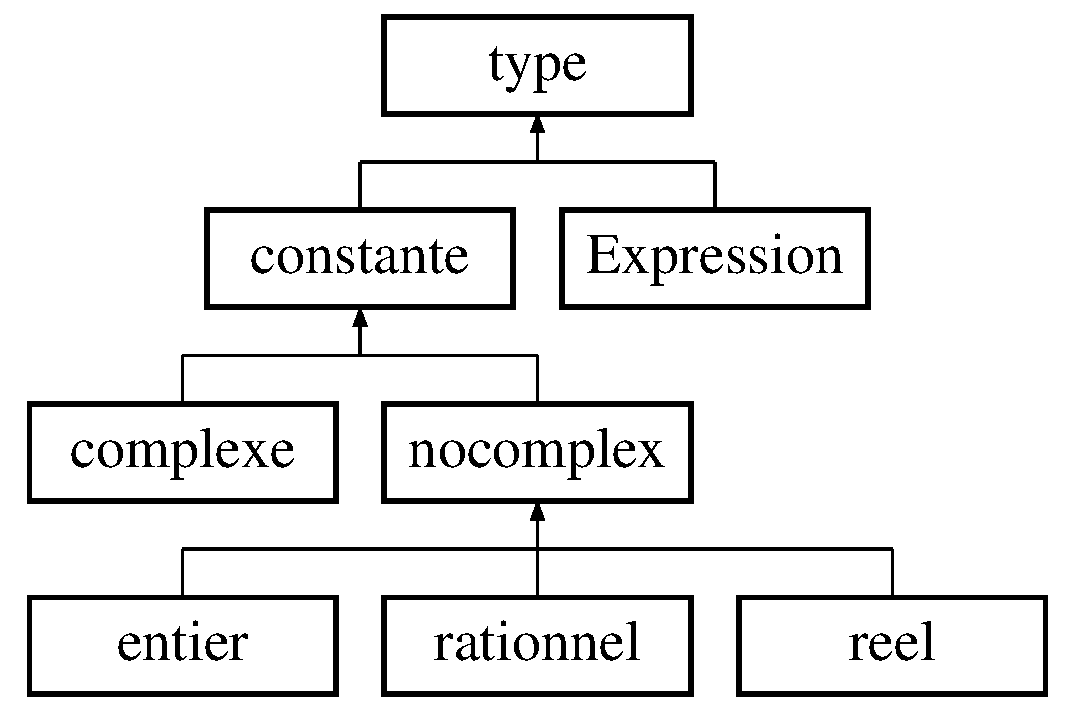
\includegraphics[height=4.000000cm]{classtype}
\end{center}
\end{figure}
\subsection*{Public Member Functions}
\begin{DoxyCompactItemize}
\item 
\hypertarget{classtype_a24236b97ec65acd7624c81fc33305e7c}{\hyperlink{classtype_a24236b97ec65acd7624c81fc33305e7c}{type} ()}\label{classtype_a24236b97ec65acd7624c81fc33305e7c}

\begin{DoxyCompactList}\small\item\em Constructeur. \end{DoxyCompactList}\item 
\hypertarget{classtype_a87f20c8ea87a2752a61aacd9a818ae8e}{virtual \hyperlink{classtype_a87f20c8ea87a2752a61aacd9a818ae8e}{$\sim$type} ()}\label{classtype_a87f20c8ea87a2752a61aacd9a818ae8e}

\begin{DoxyCompactList}\small\item\em Destructeur (virtuel) \end{DoxyCompactList}\item 
virtual \hyperlink{classtype}{type} $\ast$ \hyperlink{classtype_aae435de533d21af297434702fd71d04d}{operator+} (\hyperlink{classtype}{type} \&t)=0
\begin{DoxyCompactList}\small\item\em Operateur + Operateur binaire + Methode virtuelle pure. \end{DoxyCompactList}\item 
virtual \hyperlink{classtype}{type} $\ast$ \hyperlink{classtype_a0fad8179d45b9bbde90b48e1950ce639}{operator/} (\hyperlink{classtype}{type} \&t)=0
\begin{DoxyCompactList}\small\item\em Operateur / Operateur binaire / Methode virtuelle pure. \end{DoxyCompactList}\item 
virtual \hyperlink{classtype}{type} $\ast$ \hyperlink{classtype_a9e275d2b8465d6085515f58aaf631ea7}{operator$\ast$} (\hyperlink{classtype}{type} \&t)=0
\begin{DoxyCompactList}\small\item\em Operateur $\ast$ Operateur binaire $\ast$ Methode virtuelle pure. \end{DoxyCompactList}\item 
virtual \hyperlink{classtype}{type} $\ast$ \hyperlink{classtype_a4d440ee89d624d7314786d8d18751588}{operator-\/} (\hyperlink{classtype}{type} \&t)=0
\begin{DoxyCompactList}\small\item\em Operateur -\/ Operateur binaire -\/ Methode virtuelle pure. \end{DoxyCompactList}\item 
virtual \hyperlink{classtype}{type} $\ast$ \hyperlink{classtype_a01ae853856fcd929e5455b460ccd0be6}{pow} (\hyperlink{classtype}{type} \&t)
\begin{DoxyCompactList}\small\item\em Pow Operateur binaire Pow Methode virtuelle pure. \end{DoxyCompactList}\item 
virtual \hyperlink{classtype}{type} $\ast$ \hyperlink{classtype_aed752df353b43b17d3f993d4b02f216b}{mod} (\hyperlink{classtype}{type} \&t)
\begin{DoxyCompactList}\small\item\em Mod Operateur binaire Modulo Methode virtuelle. \end{DoxyCompactList}\item 
virtual \hyperlink{classtype}{type} $\ast$ \hyperlink{classtype_a3ec9f31aec3ddc52efe2adff634a671a}{sign} ()
\begin{DoxyCompactList}\small\item\em sign Operateur unaire sign Methode virtuelle \end{DoxyCompactList}\item 
virtual \hyperlink{classtype}{type} $\ast$ \hyperlink{classtype_acfff98100e9af7fe51f22ca553b49652}{sinus} (bool degre=false)
\begin{DoxyCompactList}\small\item\em sinus Operateur unaire sinus Methode virtuelle \end{DoxyCompactList}\item 
virtual \hyperlink{classtype}{type} $\ast$ \hyperlink{classtype_a4bf0be87d5e0314cc6a29ce86930d34e}{cosinus} (bool degre=false)
\begin{DoxyCompactList}\small\item\em cosinus Operateur unaire cosinus Methode virtuelle \end{DoxyCompactList}\item 
virtual \hyperlink{classtype}{type} $\ast$ \hyperlink{classtype_a0e48cd1a39419994f14550b2fd188e1d}{tangente} (bool degre=false)
\begin{DoxyCompactList}\small\item\em tangente Operateur unaire tangente Methode virtuelle \end{DoxyCompactList}\item 
virtual \hyperlink{classtype}{type} $\ast$ \hyperlink{classtype_a1bb104502962725e2d8d1909a208e7fa}{sinush} (bool degre=false)
\begin{DoxyCompactList}\small\item\em sinush Operateur unaire sinush Methode virtuelle \end{DoxyCompactList}\item 
virtual \hyperlink{classtype}{type} $\ast$ \hyperlink{classtype_a387836cc1a0dd2a20ece2f721fab822a}{cosinush} (bool degre=false)
\begin{DoxyCompactList}\small\item\em cosinush Operateur unaire cosinush Methode virtuelle \end{DoxyCompactList}\item 
virtual \hyperlink{classtype}{type} $\ast$ \hyperlink{classtype_a36763dd363a8de97e4a52aa87776e61c}{tangenteh} (bool degre=false)
\begin{DoxyCompactList}\small\item\em tangenteh Operateur unaire tangenteh Methode virtuelle \end{DoxyCompactList}\item 
virtual \hyperlink{classtype}{type} $\ast$ \hyperlink{classtype_aba57b52b37f984806842df5478b2489c}{ln} ()
\begin{DoxyCompactList}\small\item\em ln Operateur unaire ln Methode virtuelle \end{DoxyCompactList}\item 
virtual \hyperlink{classtype}{type} $\ast$ \hyperlink{classtype_ab02a7131b07f81a545beb9ae499bcef6}{log} ()
\begin{DoxyCompactList}\small\item\em log Operateur unaire log Methode virtuelle \end{DoxyCompactList}\item 
virtual \hyperlink{classtype}{type} $\ast$ \hyperlink{classtype_af4bf1a878929fb77f6e1edf90d33a275}{inv} ()
\begin{DoxyCompactList}\small\item\em inv Operateur unaire inv Methode virtuelle \end{DoxyCompactList}\item 
virtual \hyperlink{classtype}{type} $\ast$ \hyperlink{classtype_aedd0df2ba42b6cb66ee3dba28309a47b}{sqrt} ()
\begin{DoxyCompactList}\small\item\em sqrt Operateur unaire sqrt Methode virtuelle \end{DoxyCompactList}\item 
virtual \hyperlink{classtype}{type} $\ast$ \hyperlink{classtype_a70b655b274b3378154cd29127c22a4f0}{sqr} ()
\begin{DoxyCompactList}\small\item\em sqr Operateur unaire sqr Methode virtuelle \end{DoxyCompactList}\item 
virtual \hyperlink{classtype}{type} $\ast$ \hyperlink{classtype_ac470662477ea88722b58e98fee3e1ec0}{cube} ()
\begin{DoxyCompactList}\small\item\em cube Operateur unaire cube Methode virtuelle \end{DoxyCompactList}\item 
virtual \hyperlink{classtype}{type} $\ast$ \hyperlink{classtype_adfeadf5e6478f3687bcaba9cf9aaf8d9}{fact} ()
\begin{DoxyCompactList}\small\item\em fact Operateur unaire fact Methode virtuelle \end{DoxyCompactList}\item 
virtual Q\-String \hyperlink{classtype_a8288e5361dba59212d1f2490f6531793}{eval} ()
\begin{DoxyCompactList}\small\item\em sign Operateur unaire sign Methode virtuelle \end{DoxyCompactList}\item 
virtual Q\-String \hyperlink{classtype_ab61f01d56f3896cc99788a1a18c4b0c2}{to\-Q\-String} ()=0
\begin{DoxyCompactList}\small\item\em to\-Q\-String Methode virtuelle pure \end{DoxyCompactList}\end{DoxyCompactItemize}
\subsection*{Static Public Member Functions}
\begin{DoxyCompactItemize}
\item 
static bool \hyperlink{classtype_a011e2bd55a2d7784a1455bbc2fbba2e5}{is\-Entier} (const Q\-String \&s)
\begin{DoxyCompactList}\small\item\em is\-Entier Methode statique permettant de determiner le type (Utiisation de regexp) \end{DoxyCompactList}\item 
static bool \hyperlink{classtype_ae610cb80e031c43ae3c56033ec95a3a7}{is\-Reel} (const Q\-String \&s)
\begin{DoxyCompactList}\small\item\em is\-Reel Methode statique permettant de determiner le type (Utiisation de regexp) \end{DoxyCompactList}\item 
static bool \hyperlink{classtype_a8f2852f004b9d1676aa8ee4385d4ed49}{is\-Rationnel} (const Q\-String \&s)
\begin{DoxyCompactList}\small\item\em is\-Rationnel Methode statique permettant de determiner le type (Utiisation de regexp) \end{DoxyCompactList}\item 
static bool \hyperlink{classtype_a095a592d75acdef11c9e01e199c49e33}{is\-Expression} (const Q\-String \&s)
\begin{DoxyCompactList}\small\item\em is\-Expression Methode statique permettant de determiner le type (Utiisation de regexp) \end{DoxyCompactList}\item 
static bool \hyperlink{classtype_aeadbcfa313ab5a235bb44cf724c3ccba}{is\-Complexe} (const Q\-String \&s)
\begin{DoxyCompactList}\small\item\em is\-Complexe Methode statique permettant de determiner le type (Utiisation de regexp) \end{DoxyCompactList}\end{DoxyCompactItemize}


\subsection{Detailed Description}
Classe representant un type. 

Super Classe Abstraite utilise pour le polymorphisme 

\subsection{Member Function Documentation}
\hypertarget{classtype_a4bf0be87d5e0314cc6a29ce86930d34e}{\index{type@{type}!cosinus@{cosinus}}
\index{cosinus@{cosinus}!type@{type}}
\subsubsection[{cosinus}]{\setlength{\rightskip}{0pt plus 5cm}virtual {\bf type}$\ast$ type\-::cosinus (
\begin{DoxyParamCaption}
\item[{bool}]{degre = {\ttfamily false}}
\end{DoxyParamCaption}
)\hspace{0.3cm}{\ttfamily [inline]}, {\ttfamily [virtual]}}}\label{classtype_a4bf0be87d5e0314cc6a29ce86930d34e}


cosinus Operateur unaire cosinus Methode virtuelle 

\begin{DoxyReturn}{Returns}
Pointeur sur type, resultat de l'operation 
\end{DoxyReturn}


Reimplemented in \hyperlink{classentier_a1313e6cfa480cab69942f9b97418e491}{entier}, \hyperlink{classrationnel_a4a2f7528592b31a367799a79c336395c}{rationnel}, \hyperlink{class_expression_ab33831fb9207ba778ae46f49b2f0f7ac}{Expression}, \hyperlink{classreel_ab1d6bb643ca3335b8cb19e1b7eb89878}{reel}, and \hyperlink{classnocomplex_a2c3aa4791fe0c123079b0332a5978939}{nocomplex}.

\hypertarget{classtype_a387836cc1a0dd2a20ece2f721fab822a}{\index{type@{type}!cosinush@{cosinush}}
\index{cosinush@{cosinush}!type@{type}}
\subsubsection[{cosinush}]{\setlength{\rightskip}{0pt plus 5cm}virtual {\bf type}$\ast$ type\-::cosinush (
\begin{DoxyParamCaption}
\item[{bool}]{degre = {\ttfamily false}}
\end{DoxyParamCaption}
)\hspace{0.3cm}{\ttfamily [inline]}, {\ttfamily [virtual]}}}\label{classtype_a387836cc1a0dd2a20ece2f721fab822a}


cosinush Operateur unaire cosinush Methode virtuelle 

\begin{DoxyReturn}{Returns}
Pointeur sur type, resultat de l'operation 
\end{DoxyReturn}


Reimplemented in \hyperlink{classentier_af111db8d7c89d47f20c59e3bd0ef1dfd}{entier}, \hyperlink{classrationnel_af8de9bc6850dc5471d2e31ddf8e3866e}{rationnel}, \hyperlink{class_expression_a032591ce129e8d11b9a75c55287323d8}{Expression}, \hyperlink{classreel_a94a01afa4662790da504857247837160}{reel}, and \hyperlink{classnocomplex_ae92516f1c7c78298a11e8e34355b9f81}{nocomplex}.

\hypertarget{classtype_ac470662477ea88722b58e98fee3e1ec0}{\index{type@{type}!cube@{cube}}
\index{cube@{cube}!type@{type}}
\subsubsection[{cube}]{\setlength{\rightskip}{0pt plus 5cm}virtual {\bf type}$\ast$ type\-::cube (
\begin{DoxyParamCaption}
{}
\end{DoxyParamCaption}
)\hspace{0.3cm}{\ttfamily [inline]}, {\ttfamily [virtual]}}}\label{classtype_ac470662477ea88722b58e98fee3e1ec0}


cube Operateur unaire cube Methode virtuelle 

\begin{DoxyReturn}{Returns}
Pointeur sur type, resultat de l'operation 
\end{DoxyReturn}


Reimplemented in \hyperlink{classentier_a4c726d947d2f7464ec858f50054118e8}{entier}, \hyperlink{classrationnel_a9bca6086c4a5083765d87324418a86ab}{rationnel}, \hyperlink{class_expression_afaa9e88c0eedebcd346859b7593f5b48}{Expression}, \hyperlink{classreel_a3a2dc28d66ee81177a986fca957f6fd5}{reel}, and \hyperlink{classnocomplex_ad84e4a7a269024da4551a8e99078e41d}{nocomplex}.

\hypertarget{classtype_a8288e5361dba59212d1f2490f6531793}{\index{type@{type}!eval@{eval}}
\index{eval@{eval}!type@{type}}
\subsubsection[{eval}]{\setlength{\rightskip}{0pt plus 5cm}virtual Q\-String type\-::eval (
\begin{DoxyParamCaption}
{}
\end{DoxyParamCaption}
)\hspace{0.3cm}{\ttfamily [inline]}, {\ttfamily [virtual]}}}\label{classtype_a8288e5361dba59212d1f2490f6531793}


sign Operateur unaire sign Methode virtuelle 

\begin{DoxyReturn}{Returns}
Pointeur sur type, resultat de l'operation 
\end{DoxyReturn}


Reimplemented in \hyperlink{classrationnel_a1418b1d6ac37f7948affefa7b8d0f314}{rationnel}, \hyperlink{class_expression_a7312cb958b6366f84fb4e01f58cd2119}{Expression}, and \hyperlink{classnocomplex_a8831dff2cd793c03618b6e0751ffc026}{nocomplex}.

\hypertarget{classtype_adfeadf5e6478f3687bcaba9cf9aaf8d9}{\index{type@{type}!fact@{fact}}
\index{fact@{fact}!type@{type}}
\subsubsection[{fact}]{\setlength{\rightskip}{0pt plus 5cm}virtual {\bf type}$\ast$ type\-::fact (
\begin{DoxyParamCaption}
{}
\end{DoxyParamCaption}
)\hspace{0.3cm}{\ttfamily [inline]}, {\ttfamily [virtual]}}}\label{classtype_adfeadf5e6478f3687bcaba9cf9aaf8d9}


fact Operateur unaire fact Methode virtuelle 

\begin{DoxyReturn}{Returns}
Pointeur sur type, resultat de l'operation 
\end{DoxyReturn}


Reimplemented in \hyperlink{classentier_a8a475a326fc2c4e1b2a03ec437270144}{entier}.

\hypertarget{classtype_af4bf1a878929fb77f6e1edf90d33a275}{\index{type@{type}!inv@{inv}}
\index{inv@{inv}!type@{type}}
\subsubsection[{inv}]{\setlength{\rightskip}{0pt plus 5cm}virtual {\bf type}$\ast$ type\-::inv (
\begin{DoxyParamCaption}
{}
\end{DoxyParamCaption}
)\hspace{0.3cm}{\ttfamily [inline]}, {\ttfamily [virtual]}}}\label{classtype_af4bf1a878929fb77f6e1edf90d33a275}


inv Operateur unaire inv Methode virtuelle 

\begin{DoxyReturn}{Returns}
Pointeur sur type, resultat de l'operation 
\end{DoxyReturn}


Reimplemented in \hyperlink{classentier_abaa5775172cf9c417ccdb174304056b3}{entier}, \hyperlink{classrationnel_a75336cd670c61195c833f8459c02c3b5}{rationnel}, \hyperlink{class_expression_ab3dc93b84bb845663383b4347550c9d5}{Expression}, \hyperlink{classreel_ab863c6b28a5345dbf7657b4b5121c2f7}{reel}, and \hyperlink{classnocomplex_a9e0f97f51c50b11022c6d0b409c26ecf}{nocomplex}.

\hypertarget{classtype_aeadbcfa313ab5a235bb44cf724c3ccba}{\index{type@{type}!is\-Complexe@{is\-Complexe}}
\index{is\-Complexe@{is\-Complexe}!type@{type}}
\subsubsection[{is\-Complexe}]{\setlength{\rightskip}{0pt plus 5cm}static bool type\-::is\-Complexe (
\begin{DoxyParamCaption}
\item[{const Q\-String \&}]{s}
\end{DoxyParamCaption}
)\hspace{0.3cm}{\ttfamily [inline]}, {\ttfamily [static]}}}\label{classtype_aeadbcfa313ab5a235bb44cf724c3ccba}


is\-Complexe Methode statique permettant de determiner le type (Utiisation de regexp) 


\begin{DoxyParams}{Parameters}
{\em Qstring} & s, chaine de caractere source \\
\hline
\end{DoxyParams}
\begin{DoxyReturn}{Returns}
true si la chaine ressemble a un complexe, false sinon 
\end{DoxyReturn}
\hypertarget{classtype_a011e2bd55a2d7784a1455bbc2fbba2e5}{\index{type@{type}!is\-Entier@{is\-Entier}}
\index{is\-Entier@{is\-Entier}!type@{type}}
\subsubsection[{is\-Entier}]{\setlength{\rightskip}{0pt plus 5cm}static bool type\-::is\-Entier (
\begin{DoxyParamCaption}
\item[{const Q\-String \&}]{s}
\end{DoxyParamCaption}
)\hspace{0.3cm}{\ttfamily [inline]}, {\ttfamily [static]}}}\label{classtype_a011e2bd55a2d7784a1455bbc2fbba2e5}


is\-Entier Methode statique permettant de determiner le type (Utiisation de regexp) 


\begin{DoxyParams}{Parameters}
{\em Qstring} & s, chaine de caractere source \\
\hline
\end{DoxyParams}
\begin{DoxyReturn}{Returns}
true si la chaine ressemble a un entier, false sinon 
\end{DoxyReturn}
\hypertarget{classtype_a095a592d75acdef11c9e01e199c49e33}{\index{type@{type}!is\-Expression@{is\-Expression}}
\index{is\-Expression@{is\-Expression}!type@{type}}
\subsubsection[{is\-Expression}]{\setlength{\rightskip}{0pt plus 5cm}static bool type\-::is\-Expression (
\begin{DoxyParamCaption}
\item[{const Q\-String \&}]{s}
\end{DoxyParamCaption}
)\hspace{0.3cm}{\ttfamily [inline]}, {\ttfamily [static]}}}\label{classtype_a095a592d75acdef11c9e01e199c49e33}


is\-Expression Methode statique permettant de determiner le type (Utiisation de regexp) 


\begin{DoxyParams}{Parameters}
{\em Qstring} & s, chaine de caractere source \\
\hline
\end{DoxyParams}
\begin{DoxyReturn}{Returns}
true si la chaine ressemble a une expression, false sinon 
\end{DoxyReturn}
\hypertarget{classtype_a8f2852f004b9d1676aa8ee4385d4ed49}{\index{type@{type}!is\-Rationnel@{is\-Rationnel}}
\index{is\-Rationnel@{is\-Rationnel}!type@{type}}
\subsubsection[{is\-Rationnel}]{\setlength{\rightskip}{0pt plus 5cm}static bool type\-::is\-Rationnel (
\begin{DoxyParamCaption}
\item[{const Q\-String \&}]{s}
\end{DoxyParamCaption}
)\hspace{0.3cm}{\ttfamily [inline]}, {\ttfamily [static]}}}\label{classtype_a8f2852f004b9d1676aa8ee4385d4ed49}


is\-Rationnel Methode statique permettant de determiner le type (Utiisation de regexp) 


\begin{DoxyParams}{Parameters}
{\em Qstring} & s, chaine de caractere source \\
\hline
\end{DoxyParams}
\begin{DoxyReturn}{Returns}
true si la chaine ressemble a un rationnel, false sinon 
\end{DoxyReturn}
\hypertarget{classtype_ae610cb80e031c43ae3c56033ec95a3a7}{\index{type@{type}!is\-Reel@{is\-Reel}}
\index{is\-Reel@{is\-Reel}!type@{type}}
\subsubsection[{is\-Reel}]{\setlength{\rightskip}{0pt plus 5cm}static bool type\-::is\-Reel (
\begin{DoxyParamCaption}
\item[{const Q\-String \&}]{s}
\end{DoxyParamCaption}
)\hspace{0.3cm}{\ttfamily [inline]}, {\ttfamily [static]}}}\label{classtype_ae610cb80e031c43ae3c56033ec95a3a7}


is\-Reel Methode statique permettant de determiner le type (Utiisation de regexp) 


\begin{DoxyParams}{Parameters}
{\em Qstring} & s, chaine de caractere source \\
\hline
\end{DoxyParams}
\begin{DoxyReturn}{Returns}
true si la chaine ressemble a un reel, false sinon 
\end{DoxyReturn}
\hypertarget{classtype_aba57b52b37f984806842df5478b2489c}{\index{type@{type}!ln@{ln}}
\index{ln@{ln}!type@{type}}
\subsubsection[{ln}]{\setlength{\rightskip}{0pt plus 5cm}virtual {\bf type}$\ast$ type\-::ln (
\begin{DoxyParamCaption}
{}
\end{DoxyParamCaption}
)\hspace{0.3cm}{\ttfamily [inline]}, {\ttfamily [virtual]}}}\label{classtype_aba57b52b37f984806842df5478b2489c}


ln Operateur unaire ln Methode virtuelle 

\begin{DoxyReturn}{Returns}
Pointeur sur type, resultat de l'operation 
\end{DoxyReturn}


Reimplemented in \hyperlink{classentier_aef2c65b9f379c5ea7857fcaabca30dba}{entier}, \hyperlink{classrationnel_a59b1b593905de8676db02d5d2a5554c3}{rationnel}, \hyperlink{class_expression_a1f6cd71d574995f2c3e80c3033ca2940}{Expression}, \hyperlink{classreel_a5d09de0b7e0856eb63d333f766c770ed}{reel}, and \hyperlink{classnocomplex_ab3e91b96595fef9d53a5cfb93291c8f0}{nocomplex}.

\hypertarget{classtype_ab02a7131b07f81a545beb9ae499bcef6}{\index{type@{type}!log@{log}}
\index{log@{log}!type@{type}}
\subsubsection[{log}]{\setlength{\rightskip}{0pt plus 5cm}virtual {\bf type}$\ast$ type\-::log (
\begin{DoxyParamCaption}
{}
\end{DoxyParamCaption}
)\hspace{0.3cm}{\ttfamily [inline]}, {\ttfamily [virtual]}}}\label{classtype_ab02a7131b07f81a545beb9ae499bcef6}


log Operateur unaire log Methode virtuelle 

\begin{DoxyReturn}{Returns}
Pointeur sur type, resultat de l'operation 
\end{DoxyReturn}


Reimplemented in \hyperlink{classentier_aeca6cf72ceaa32cfc7b52f00d962d3cc}{entier}, \hyperlink{classrationnel_a6bed14bda0b8546528454e7b2030645d}{rationnel}, \hyperlink{class_expression_a9eb28aee26ef54093fc83f89ef3c1523}{Expression}, \hyperlink{classreel_adcf600e2052329def8e10e81e35ef96e}{reel}, and \hyperlink{classnocomplex_a0f7a5802123786d1461271d5c05158ca}{nocomplex}.

\hypertarget{classtype_aed752df353b43b17d3f993d4b02f216b}{\index{type@{type}!mod@{mod}}
\index{mod@{mod}!type@{type}}
\subsubsection[{mod}]{\setlength{\rightskip}{0pt plus 5cm}virtual {\bf type}$\ast$ type\-::mod (
\begin{DoxyParamCaption}
\item[{{\bf type} \&}]{t}
\end{DoxyParamCaption}
)\hspace{0.3cm}{\ttfamily [inline]}, {\ttfamily [virtual]}}}\label{classtype_aed752df353b43b17d3f993d4b02f216b}


Mod Operateur binaire Modulo Methode virtuelle. 


\begin{DoxyParams}{Parameters}
{\em t} & \-: Pointeur sur un type \\
\hline
\end{DoxyParams}
\begin{DoxyReturn}{Returns}
Pointeur sur type, resultat de l'operation 
\end{DoxyReturn}


Reimplemented in \hyperlink{classentier_a4e5c25c0ed52135136bb75563a9337e7}{entier}, and \hyperlink{class_expression_ac46a4b88a1b08206e08da229fdbfd3e9}{Expression}.

\hypertarget{classtype_a9e275d2b8465d6085515f58aaf631ea7}{\index{type@{type}!operator$\ast$@{operator$\ast$}}
\index{operator$\ast$@{operator$\ast$}!type@{type}}
\subsubsection[{operator$\ast$}]{\setlength{\rightskip}{0pt plus 5cm}virtual {\bf type}$\ast$ type\-::operator$\ast$ (
\begin{DoxyParamCaption}
\item[{{\bf type} \&}]{t}
\end{DoxyParamCaption}
)\hspace{0.3cm}{\ttfamily [pure virtual]}}}\label{classtype_a9e275d2b8465d6085515f58aaf631ea7}


Operateur $\ast$ Operateur binaire $\ast$ Methode virtuelle pure. 


\begin{DoxyParams}{Parameters}
{\em t} & \-: Pointeur sur un type \\
\hline
\end{DoxyParams}
\begin{DoxyReturn}{Returns}
Pointeur sur type, resultat de l'operation 
\end{DoxyReturn}


Implemented in \hyperlink{classcomplexe_a02371b6578996af8af11f260931259b4}{complexe}, \hyperlink{classentier_a7314a5aad4a2c997eaea01e3aa42092a}{entier}, \hyperlink{classreel_a044791a71fd9926cbedf3f19f6eea122}{reel}, \hyperlink{classrationnel_a49250cb9001aad230e5193515ee74efa}{rationnel}, \hyperlink{class_expression_a9f63512e41bb2e498951342759a6fa1e}{Expression}, and \hyperlink{classnocomplex_ac84954cbe0bd9c77eab88c0b97b34c2b}{nocomplex}.

\hypertarget{classtype_aae435de533d21af297434702fd71d04d}{\index{type@{type}!operator+@{operator+}}
\index{operator+@{operator+}!type@{type}}
\subsubsection[{operator+}]{\setlength{\rightskip}{0pt plus 5cm}virtual {\bf type}$\ast$ type\-::operator+ (
\begin{DoxyParamCaption}
\item[{{\bf type} \&}]{t}
\end{DoxyParamCaption}
)\hspace{0.3cm}{\ttfamily [pure virtual]}}}\label{classtype_aae435de533d21af297434702fd71d04d}


Operateur + Operateur binaire + Methode virtuelle pure. 


\begin{DoxyParams}{Parameters}
{\em t} & \-: Pointeur sur un type \\
\hline
\end{DoxyParams}
\begin{DoxyReturn}{Returns}
Pointeur sur type, resultat de l'operation 
\end{DoxyReturn}


Implemented in \hyperlink{classcomplexe_a9f98da0548d8b73f1f10f248061d196b}{complexe}, \hyperlink{classentier_a531e654172d6e2fe225fad108dbb84a7}{entier}, \hyperlink{classreel_af2ae884e68ab28b286cf9940f05f59d9}{reel}, \hyperlink{classrationnel_a14d9d411058e146e075ccf16997e525e}{rationnel}, \hyperlink{class_expression_a1572f9f1d8b2619b14d7d58f72a63e22}{Expression}, and \hyperlink{classnocomplex_af3d04b00f4f82d3a35cad0ca023093f4}{nocomplex}.

\hypertarget{classtype_a4d440ee89d624d7314786d8d18751588}{\index{type@{type}!operator-\/@{operator-\/}}
\index{operator-\/@{operator-\/}!type@{type}}
\subsubsection[{operator-\/}]{\setlength{\rightskip}{0pt plus 5cm}virtual {\bf type}$\ast$ type\-::operator-\/ (
\begin{DoxyParamCaption}
\item[{{\bf type} \&}]{t}
\end{DoxyParamCaption}
)\hspace{0.3cm}{\ttfamily [pure virtual]}}}\label{classtype_a4d440ee89d624d7314786d8d18751588}


Operateur -\/ Operateur binaire -\/ Methode virtuelle pure. 


\begin{DoxyParams}{Parameters}
{\em t} & \-: Pointeur sur un type \\
\hline
\end{DoxyParams}
\begin{DoxyReturn}{Returns}
Pointeur sur type, resultat de l'operation 
\end{DoxyReturn}


Implemented in \hyperlink{classcomplexe_ae74ae6a7236ccbdaf74e88e5464ffb43}{complexe}, \hyperlink{classentier_ac0acf2b6156ef6f5f2e034c0425e1114}{entier}, \hyperlink{classreel_a9cd96b762004392eda5216262201322c}{reel}, \hyperlink{classrationnel_a3bdf6de1a2526ddafbf1831a9af11dc9}{rationnel}, \hyperlink{class_expression_adb495f245e3652e3605b290d7d41acb5}{Expression}, and \hyperlink{classnocomplex_a2005c3a0fcaa1f360561539931ffc578}{nocomplex}.

\hypertarget{classtype_a0fad8179d45b9bbde90b48e1950ce639}{\index{type@{type}!operator/@{operator/}}
\index{operator/@{operator/}!type@{type}}
\subsubsection[{operator/}]{\setlength{\rightskip}{0pt plus 5cm}virtual {\bf type}$\ast$ type\-::operator/ (
\begin{DoxyParamCaption}
\item[{{\bf type} \&}]{t}
\end{DoxyParamCaption}
)\hspace{0.3cm}{\ttfamily [pure virtual]}}}\label{classtype_a0fad8179d45b9bbde90b48e1950ce639}


Operateur / Operateur binaire / Methode virtuelle pure. 


\begin{DoxyParams}{Parameters}
{\em t} & \-: Pointeur sur un type \\
\hline
\end{DoxyParams}
\begin{DoxyReturn}{Returns}
Pointeur sur type, resultat de l'operation 
\end{DoxyReturn}


Implemented in \hyperlink{classcomplexe_af2faf54f25b3e58699ecf1d0b6409603}{complexe}, \hyperlink{classentier_a3bfd34b6998c5c09df0dbbadead47867}{entier}, \hyperlink{classreel_a3bc55f29b377547040d47be018b73fe6}{reel}, \hyperlink{classrationnel_ae36b04407cc70d425ed0292975b0d1e9}{rationnel}, \hyperlink{class_expression_aeb3e786f0524b1b1e2c5b238c8d2e50c}{Expression}, and \hyperlink{classnocomplex_a47942bdcc78cfc5d5e867c9f9836a465}{nocomplex}.

\hypertarget{classtype_a01ae853856fcd929e5455b460ccd0be6}{\index{type@{type}!pow@{pow}}
\index{pow@{pow}!type@{type}}
\subsubsection[{pow}]{\setlength{\rightskip}{0pt plus 5cm}virtual {\bf type}$\ast$ type\-::pow (
\begin{DoxyParamCaption}
\item[{{\bf type} \&}]{t}
\end{DoxyParamCaption}
)\hspace{0.3cm}{\ttfamily [inline]}, {\ttfamily [virtual]}}}\label{classtype_a01ae853856fcd929e5455b460ccd0be6}


Pow Operateur binaire Pow Methode virtuelle pure. 


\begin{DoxyParams}{Parameters}
{\em t} & \-: Pointeur sur un type \\
\hline
\end{DoxyParams}
\begin{DoxyReturn}{Returns}
Pointeur sur type, resultat de l'operation 
\end{DoxyReturn}


Reimplemented in \hyperlink{classentier_adc71e10e6ea385f7c1aa1de06e2d1b4c}{entier}, \hyperlink{classrationnel_afd9fd9a30f034952ce889d46a07de617}{rationnel}, \hyperlink{classreel_a4fdea6a69bd78b2593fb44cc172fc7bf}{reel}, \hyperlink{class_expression_aeaf521221894a0012b604cc0033518b9}{Expression}, and \hyperlink{classnocomplex_a1ad1b692783c8449efb03cc0dc5d1f3c}{nocomplex}.

\hypertarget{classtype_a3ec9f31aec3ddc52efe2adff634a671a}{\index{type@{type}!sign@{sign}}
\index{sign@{sign}!type@{type}}
\subsubsection[{sign}]{\setlength{\rightskip}{0pt plus 5cm}virtual {\bf type}$\ast$ type\-::sign (
\begin{DoxyParamCaption}
{}
\end{DoxyParamCaption}
)\hspace{0.3cm}{\ttfamily [inline]}, {\ttfamily [virtual]}}}\label{classtype_a3ec9f31aec3ddc52efe2adff634a671a}


sign Operateur unaire sign Methode virtuelle 

\begin{DoxyReturn}{Returns}
Pointeur sur type, resultat de l'operation 
\end{DoxyReturn}


Reimplemented in \hyperlink{classentier_a4a25b08f29eba0a531bebadeaf77ee04}{entier}, \hyperlink{classrationnel_aa73709167be428fafc4d95a31f4c3cc0}{rationnel}, \hyperlink{class_expression_aa654b4e71cfafd29af080020a77dc1e0}{Expression}, \hyperlink{classreel_a9a172c44e0a496059bdd1c4d53a98590}{reel}, \hyperlink{classcomplexe_a9e7f59cfa1dd74f77891d7bfd1c1c62b}{complexe}, and \hyperlink{classnocomplex_acd1c0365d1a2ed160934320cff01cecd}{nocomplex}.

\hypertarget{classtype_acfff98100e9af7fe51f22ca553b49652}{\index{type@{type}!sinus@{sinus}}
\index{sinus@{sinus}!type@{type}}
\subsubsection[{sinus}]{\setlength{\rightskip}{0pt plus 5cm}virtual {\bf type}$\ast$ type\-::sinus (
\begin{DoxyParamCaption}
\item[{bool}]{degre = {\ttfamily false}}
\end{DoxyParamCaption}
)\hspace{0.3cm}{\ttfamily [inline]}, {\ttfamily [virtual]}}}\label{classtype_acfff98100e9af7fe51f22ca553b49652}


sinus Operateur unaire sinus Methode virtuelle 

\begin{DoxyReturn}{Returns}
Pointeur sur type, resultat de l'operation 
\end{DoxyReturn}


Reimplemented in \hyperlink{classentier_a5dd86ffdc48bf745871ac2f65199d2ce}{entier}, \hyperlink{classreel_a3502ff761467546024da46f1f2bbb2e7}{reel}, \hyperlink{classrationnel_ad34af896f760a0271286e2dbbf55ad9f}{rationnel}, \hyperlink{class_expression_a67a5046f6af705fef094ff5e4a78880d}{Expression}, and \hyperlink{classnocomplex_aea2ba416f34c37ad2cf751b6220d53b8}{nocomplex}.

\hypertarget{classtype_a1bb104502962725e2d8d1909a208e7fa}{\index{type@{type}!sinush@{sinush}}
\index{sinush@{sinush}!type@{type}}
\subsubsection[{sinush}]{\setlength{\rightskip}{0pt plus 5cm}virtual {\bf type}$\ast$ type\-::sinush (
\begin{DoxyParamCaption}
\item[{bool}]{degre = {\ttfamily false}}
\end{DoxyParamCaption}
)\hspace{0.3cm}{\ttfamily [inline]}, {\ttfamily [virtual]}}}\label{classtype_a1bb104502962725e2d8d1909a208e7fa}


sinush Operateur unaire sinush Methode virtuelle 

\begin{DoxyReturn}{Returns}
Pointeur sur type, resultat de l'operation 
\end{DoxyReturn}


Reimplemented in \hyperlink{classentier_abfb8840f088a4771520fd48a78c01434}{entier}, \hyperlink{classrationnel_a107f6a0be55879bd49dd015144fdfde4}{rationnel}, \hyperlink{class_expression_a45aef44cb37e21e99614053bf80801f6}{Expression}, \hyperlink{classreel_a410b5cc4316eeddbeff2ec46c13ca249}{reel}, and \hyperlink{classnocomplex_a4df698a9ee147b77aaab9f63840b1012}{nocomplex}.

\hypertarget{classtype_a70b655b274b3378154cd29127c22a4f0}{\index{type@{type}!sqr@{sqr}}
\index{sqr@{sqr}!type@{type}}
\subsubsection[{sqr}]{\setlength{\rightskip}{0pt plus 5cm}virtual {\bf type}$\ast$ type\-::sqr (
\begin{DoxyParamCaption}
{}
\end{DoxyParamCaption}
)\hspace{0.3cm}{\ttfamily [inline]}, {\ttfamily [virtual]}}}\label{classtype_a70b655b274b3378154cd29127c22a4f0}


sqr Operateur unaire sqr Methode virtuelle 

\begin{DoxyReturn}{Returns}
Pointeur sur type, resultat de l'operation 
\end{DoxyReturn}


Reimplemented in \hyperlink{classentier_a33b0b2b13a0fdc767a809df33b934dd6}{entier}, \hyperlink{classrationnel_ab9f341fd09499253dd1f9b6f15795576}{rationnel}, \hyperlink{class_expression_a172e59bd44c5ddf668fd8027f0733d8d}{Expression}, \hyperlink{classreel_ad295586d5862f6dc41966f25c365c4a1}{reel}, and \hyperlink{classnocomplex_a5665f2bcf5ad839e92c31f38f3dfc7b7}{nocomplex}.

\hypertarget{classtype_aedd0df2ba42b6cb66ee3dba28309a47b}{\index{type@{type}!sqrt@{sqrt}}
\index{sqrt@{sqrt}!type@{type}}
\subsubsection[{sqrt}]{\setlength{\rightskip}{0pt plus 5cm}virtual {\bf type}$\ast$ type\-::sqrt (
\begin{DoxyParamCaption}
{}
\end{DoxyParamCaption}
)\hspace{0.3cm}{\ttfamily [inline]}, {\ttfamily [virtual]}}}\label{classtype_aedd0df2ba42b6cb66ee3dba28309a47b}


sqrt Operateur unaire sqrt Methode virtuelle 

\begin{DoxyReturn}{Returns}
Pointeur sur type, resultat de l'operation 
\end{DoxyReturn}


Reimplemented in \hyperlink{classentier_a9058b76c3fae96fb3a9ade24e6c33926}{entier}, \hyperlink{classrationnel_ad37ab4380b5ff66104748ecc0bf5babe}{rationnel}, \hyperlink{class_expression_ac5b9d54cc3699ccec579001a9e954bd3}{Expression}, \hyperlink{classreel_a980bc278bf5537519ee05746262ebb6a}{reel}, and \hyperlink{classnocomplex_a7f693a0869814705bcc3b8add799e6cd}{nocomplex}.

\hypertarget{classtype_a0e48cd1a39419994f14550b2fd188e1d}{\index{type@{type}!tangente@{tangente}}
\index{tangente@{tangente}!type@{type}}
\subsubsection[{tangente}]{\setlength{\rightskip}{0pt plus 5cm}virtual {\bf type}$\ast$ type\-::tangente (
\begin{DoxyParamCaption}
\item[{bool}]{degre = {\ttfamily false}}
\end{DoxyParamCaption}
)\hspace{0.3cm}{\ttfamily [inline]}, {\ttfamily [virtual]}}}\label{classtype_a0e48cd1a39419994f14550b2fd188e1d}


tangente Operateur unaire tangente Methode virtuelle 

\begin{DoxyReturn}{Returns}
Pointeur sur type, resultat de l'operation 
\end{DoxyReturn}


Reimplemented in \hyperlink{classentier_a600a48ecf8280f0ab465ab3f3c253662}{entier}, \hyperlink{classrationnel_ac2bdc47a11ea3d010f006256f6e14f79}{rationnel}, \hyperlink{class_expression_ae47f82ffeefff823064141174ba5c3ac}{Expression}, \hyperlink{classreel_a88d653b80c7d3a1a4f9c4ac4b709957b}{reel}, and \hyperlink{classnocomplex_a2e7f4563e7d602c79e356dcb5472e341}{nocomplex}.

\hypertarget{classtype_a36763dd363a8de97e4a52aa87776e61c}{\index{type@{type}!tangenteh@{tangenteh}}
\index{tangenteh@{tangenteh}!type@{type}}
\subsubsection[{tangenteh}]{\setlength{\rightskip}{0pt plus 5cm}virtual {\bf type}$\ast$ type\-::tangenteh (
\begin{DoxyParamCaption}
\item[{bool}]{degre = {\ttfamily false}}
\end{DoxyParamCaption}
)\hspace{0.3cm}{\ttfamily [inline]}, {\ttfamily [virtual]}}}\label{classtype_a36763dd363a8de97e4a52aa87776e61c}


tangenteh Operateur unaire tangenteh Methode virtuelle 

\begin{DoxyReturn}{Returns}
Pointeur sur type, resultat de l'operation 
\end{DoxyReturn}


Reimplemented in \hyperlink{classentier_abd47ffc368af385550ed2db6ce289ded}{entier}, \hyperlink{classrationnel_a56135a99618c1fec82901c5e7f64a4a2}{rationnel}, \hyperlink{class_expression_a0d0acd016a909609e451836060d4e676}{Expression}, \hyperlink{classreel_a00cb6cca23061d928135c074a5d69eb0}{reel}, and \hyperlink{classnocomplex_a79aa6c234a5a66bfe18c39794e56c277}{nocomplex}.

\hypertarget{classtype_ab61f01d56f3896cc99788a1a18c4b0c2}{\index{type@{type}!to\-Q\-String@{to\-Q\-String}}
\index{to\-Q\-String@{to\-Q\-String}!type@{type}}
\subsubsection[{to\-Q\-String}]{\setlength{\rightskip}{0pt plus 5cm}virtual Q\-String type\-::to\-Q\-String (
\begin{DoxyParamCaption}
{}
\end{DoxyParamCaption}
)\hspace{0.3cm}{\ttfamily [pure virtual]}}}\label{classtype_ab61f01d56f3896cc99788a1a18c4b0c2}


to\-Q\-String Methode virtuelle pure 

\begin{DoxyReturn}{Returns}
chaine de caractere 
\end{DoxyReturn}


Implemented in \hyperlink{classentier_a47b7c0d899f24e9117e123165648686b}{entier}, \hyperlink{class_expression_a4404792ff4997e7c06a3242062825f5c}{Expression}, \hyperlink{classrationnel_a6c905c688ae54647074a5ddf3ef648bd}{rationnel}, \hyperlink{classreel_a6b06a283958b63fde5c12382b744a8c9}{reel}, and \hyperlink{classcomplexe_a5fc10d08facdcbd833d91d0c765c9c18}{complexe}.



The documentation for this class was generated from the following file\-:\begin{DoxyCompactItemize}
\item 
Code/projet\-\_\-lo21/\hyperlink{type_8h}{type.\-h}\end{DoxyCompactItemize}

\hypertarget{classtype__factory}{\section{type\-\_\-factory Class Reference}
\label{classtype__factory}\index{type\-\_\-factory@{type\-\_\-factory}}
}


{\ttfamily \#include $<$type\-\_\-factory.\-h$>$}

\subsection*{Public Member Functions}
\begin{DoxyCompactItemize}
\item 
\hyperlink{classtype}{type} $\ast$ \hyperlink{classtype__factory_a144da545ae1616b3e9e644ad0df9564c}{get\-Type} (Q\-String s)
\end{DoxyCompactItemize}
\subsection*{Static Public Member Functions}
\begin{DoxyCompactItemize}
\item 
static \hyperlink{classtype__factory}{type\-\_\-factory} \& \hyperlink{classtype__factory_a78223a2e795f2fd36ca4b2a1666b59ec}{get\-Instance} ()
\item 
static void \hyperlink{classtype__factory_af91382fb401454be520fe8cf43ee9245}{release\-Instance} ()
\end{DoxyCompactItemize}


\subsection{Member Function Documentation}
\hypertarget{classtype__factory_a78223a2e795f2fd36ca4b2a1666b59ec}{\index{type\-\_\-factory@{type\-\_\-factory}!get\-Instance@{get\-Instance}}
\index{get\-Instance@{get\-Instance}!type_factory@{type\-\_\-factory}}
\subsubsection[{get\-Instance}]{\setlength{\rightskip}{0pt plus 5cm}{\bf type\-\_\-factory} \& type\-\_\-factory\-::get\-Instance (
\begin{DoxyParamCaption}
{}
\end{DoxyParamCaption}
)\hspace{0.3cm}{\ttfamily [static]}}}\label{classtype__factory_a78223a2e795f2fd36ca4b2a1666b59ec}
\hypertarget{classtype__factory_a144da545ae1616b3e9e644ad0df9564c}{\index{type\-\_\-factory@{type\-\_\-factory}!get\-Type@{get\-Type}}
\index{get\-Type@{get\-Type}!type_factory@{type\-\_\-factory}}
\subsubsection[{get\-Type}]{\setlength{\rightskip}{0pt plus 5cm}{\bf type} $\ast$ type\-\_\-factory\-::get\-Type (
\begin{DoxyParamCaption}
\item[{Q\-String}]{s}
\end{DoxyParamCaption}
)}}\label{classtype__factory_a144da545ae1616b3e9e644ad0df9564c}
\hypertarget{classtype__factory_af91382fb401454be520fe8cf43ee9245}{\index{type\-\_\-factory@{type\-\_\-factory}!release\-Instance@{release\-Instance}}
\index{release\-Instance@{release\-Instance}!type_factory@{type\-\_\-factory}}
\subsubsection[{release\-Instance}]{\setlength{\rightskip}{0pt plus 5cm}void type\-\_\-factory\-::release\-Instance (
\begin{DoxyParamCaption}
{}
\end{DoxyParamCaption}
)\hspace{0.3cm}{\ttfamily [static]}}}\label{classtype__factory_af91382fb401454be520fe8cf43ee9245}


The documentation for this class was generated from the following files\-:\begin{DoxyCompactItemize}
\item 
Code/projet\-\_\-lo21/\hyperlink{type__factory_8h}{type\-\_\-factory.\-h}\item 
Code/projet\-\_\-lo21/\hyperlink{type__factory_8cpp}{type\-\_\-factory.\-cpp}\end{DoxyCompactItemize}

\hypertarget{classtype_exception}{\section{type\-Exception Class Reference}
\label{classtype_exception}\index{type\-Exception@{type\-Exception}}
}


Classe d'exception pour les types.  




{\ttfamily \#include $<$typeexception.\-h$>$}

\subsection*{Public Member Functions}
\begin{DoxyCompactItemize}
\item 
\hyperlink{classtype_exception_a929459bb1b2c25570a7a8db39dc780c9}{type\-Exception} (const char $\ast$s=\char`\"{}\char`\"{})
\begin{DoxyCompactList}\small\item\em Constructeur. \end{DoxyCompactList}\item 
const char $\ast$ \hyperlink{classtype_exception_acb09e914ab67041e5aedd399b78241a7}{what} () const   throw ()
\begin{DoxyCompactList}\small\item\em what \end{DoxyCompactList}\item 
\hypertarget{classtype_exception_a9eae7b8d8c538fa64ae5f40a23ae417e}{\hyperlink{classtype_exception_a9eae7b8d8c538fa64ae5f40a23ae417e}{$\sim$type\-Exception} ()  throw ()}\label{classtype_exception_a9eae7b8d8c538fa64ae5f40a23ae417e}

\begin{DoxyCompactList}\small\item\em Destructeur. \end{DoxyCompactList}\end{DoxyCompactItemize}


\subsection{Detailed Description}
Classe d'exception pour les types. 

Derive de std\-::exception 

\subsection{Constructor \& Destructor Documentation}
\hypertarget{classtype_exception_a929459bb1b2c25570a7a8db39dc780c9}{\index{type\-Exception@{type\-Exception}!type\-Exception@{type\-Exception}}
\index{type\-Exception@{type\-Exception}!typeException@{type\-Exception}}
\subsubsection[{type\-Exception}]{\setlength{\rightskip}{0pt plus 5cm}type\-Exception\-::type\-Exception (
\begin{DoxyParamCaption}
\item[{const char $\ast$}]{s = {\ttfamily \char`\"{}\char`\"{}}}
\end{DoxyParamCaption}
)\hspace{0.3cm}{\ttfamily [inline]}}}\label{classtype_exception_a929459bb1b2c25570a7a8db39dc780c9}


Constructeur. 

Construit une exception a partir d'une chaine de caractere 

\subsection{Member Function Documentation}
\hypertarget{classtype_exception_acb09e914ab67041e5aedd399b78241a7}{\index{type\-Exception@{type\-Exception}!what@{what}}
\index{what@{what}!typeException@{type\-Exception}}
\subsubsection[{what}]{\setlength{\rightskip}{0pt plus 5cm}const char$\ast$ type\-Exception\-::what (
\begin{DoxyParamCaption}
{}
\end{DoxyParamCaption}
) const  throw ()\hspace{0.3cm}{\ttfamily [inline]}}}\label{classtype_exception_acb09e914ab67041e5aedd399b78241a7}


what 

Permet d'en savoir plus sur la cause de l'erreur \begin{DoxyReturn}{Returns}
information sur l'erreur (char $\ast$) 
\end{DoxyReturn}


The documentation for this class was generated from the following file\-:\begin{DoxyCompactItemize}
\item 
Code/projet\-\_\-lo21/\hyperlink{typeexception_8h}{typeexception.\-h}\end{DoxyCompactItemize}

\chapter{File Documentation}
\hypertarget{collection__pile_8h}{\section{Code/projet\-\_\-lo21/collection\-\_\-pile.h File Reference}
\label{collection__pile_8h}\index{Code/projet\-\_\-lo21/collection\-\_\-pile.\-h@{Code/projet\-\_\-lo21/collection\-\_\-pile.\-h}}
}


Conteneur de piles.  


{\ttfamily \#include $<$vector$>$}\\*
{\ttfamily \#include \char`\"{}pile.\-h\char`\"{}}\\*
{\ttfamily \#include $<$Q\-String$>$}\\*
\subsection*{Classes}
\begin{DoxyCompactItemize}
\item 
class \hyperlink{class_collection__pile}{Collection\-\_\-pile}
\begin{DoxyCompactList}\small\item\em Classe conteneur de piles. \end{DoxyCompactList}\end{DoxyCompactItemize}


\subsection{Detailed Description}
Conteneur de piles. \begin{DoxyAuthor}{Author}
Le Feurmou/\-Leleu 
\end{DoxyAuthor}

\hypertarget{complexe_8h}{\section{Code/projet\-\_\-lo21/complexe.h File Reference}
\label{complexe_8h}\index{Code/projet\-\_\-lo21/complexe.\-h@{Code/projet\-\_\-lo21/complexe.\-h}}
}
{\ttfamily \#include \char`\"{}type.\-h\char`\"{}}\\*
{\ttfamily \#include $<$sstream$>$}\\*
{\ttfamily \#include $<$Q\-String$>$}\\*
{\ttfamily \#include \char`\"{}nocomplex.\-h\char`\"{}}\\*
{\ttfamily \#include \char`\"{}type\-\_\-factory.\-h\char`\"{}}\\*
{\ttfamily \#include \char`\"{}constante.\-h\char`\"{}}\\*
\subsection*{Classes}
\begin{DoxyCompactItemize}
\item 
class \hyperlink{classcomplexe}{complexe}
\begin{DoxyCompactList}\small\item\em Classe representant un complexe. \end{DoxyCompactList}\end{DoxyCompactItemize}


\subsection{Detailed Description}
\begin{DoxyAuthor}{Author}
Le Feurmou/\-Leleu 
\end{DoxyAuthor}

\hypertarget{dom_8h}{\section{Code/projet\-\_\-lo21/dom.h File Reference}
\label{dom_8h}\index{Code/projet\-\_\-lo21/dom.\-h@{Code/projet\-\_\-lo21/dom.\-h}}
}
{\ttfamily \#include $<$Q\-Text\-Stream$>$}\\*
{\ttfamily \#include $<$Qt\-Xml/\-Q\-Dom\-Document$>$}\\*
{\ttfamily \#include $<$Q\-File$>$}\\*
{\ttfamily \#include $<$Q\-Message\-Box$>$}\\*
{\ttfamily \#include $<$Q\-String$>$}\\*
{\ttfamily \#include $<$Q\-Debug$>$}\\*
{\ttfamily \#include \char`\"{}pile.\-h\char`\"{}}\\*
\subsection*{Classes}
\begin{DoxyCompactItemize}
\item 
class \hyperlink{class_dom}{Dom}
\end{DoxyCompactItemize}

\hypertarget{entier_8h}{\section{Code/projet\-\_\-lo21/entier.h File Reference}
\label{entier_8h}\index{Code/projet\-\_\-lo21/entier.\-h@{Code/projet\-\_\-lo21/entier.\-h}}
}
{\ttfamily \#include \char`\"{}type.\-h\char`\"{}}\\*
{\ttfamily \#include $<$sstream$>$}\\*
{\ttfamily \#include $<$Q\-String$>$}\\*
{\ttfamily \#include \char`\"{}nocomplex.\-h\char`\"{}}\\*
{\ttfamily \#include $<$Q\-Reg\-Exp$>$}\\*
\subsection*{Classes}
\begin{DoxyCompactItemize}
\item 
class \hyperlink{classentier}{entier}
\begin{DoxyCompactList}\small\item\em Classe representant une constante. \end{DoxyCompactList}\end{DoxyCompactItemize}


\subsection{Detailed Description}
\begin{DoxyAuthor}{Author}
Le Feurmou/\-Leleu 
\end{DoxyAuthor}

\hypertarget{expression_8h}{\section{Code/projet\-\_\-lo21/expression.h File Reference}
\label{expression_8h}\index{Code/projet\-\_\-lo21/expression.\-h@{Code/projet\-\_\-lo21/expression.\-h}}
}
{\ttfamily \#include $<$Q\-String$>$}\\*
{\ttfamily \#include \char`\"{}type.\-h\char`\"{}}\\*
\subsection*{Classes}
\begin{DoxyCompactItemize}
\item 
class \hyperlink{class_expression}{Expression}
\end{DoxyCompactItemize}

\hypertarget{gardien_8h}{\section{Code/projet\-\_\-lo21/gardien.h File Reference}
\label{gardien_8h}\index{Code/projet\-\_\-lo21/gardien.\-h@{Code/projet\-\_\-lo21/gardien.\-h}}
}
{\ttfamily \#include $<$Q\-Vector$>$}\\*
{\ttfamily \#include $<$Q\-Stack$>$}\\*
{\ttfamily \#include \char`\"{}type.\-h\char`\"{}}\\*
\subsection*{Classes}
\begin{DoxyCompactItemize}
\item 
class \hyperlink{classgardien}{gardien}
\end{DoxyCompactItemize}

\hypertarget{mainwindow_8h}{\section{Code/projet\-\_\-lo21/mainwindow.h File Reference}
\label{mainwindow_8h}\index{Code/projet\-\_\-lo21/mainwindow.\-h@{Code/projet\-\_\-lo21/mainwindow.\-h}}
}
{\ttfamily \#include $<$Q\-Main\-Window$>$}\\*
{\ttfamily \#include $<$Q\-Stack$>$}\\*
{\ttfamily \#include \char`\"{}pile.\-h\char`\"{}}\\*
{\ttfamily \#include \char`\"{}type.\-h\char`\"{}}\\*
{\ttfamily \#include $<$Q\-String$>$}\\*
{\ttfamily \#include \char`\"{}reglages.\-h\char`\"{}}\\*
{\ttfamily \#include \char`\"{}collection\-\_\-pile.\-h\char`\"{}}\\*
\subsection*{Classes}
\begin{DoxyCompactItemize}
\item 
class \hyperlink{class_main_window}{Main\-Window}
\end{DoxyCompactItemize}
\subsection*{Namespaces}
\begin{DoxyCompactItemize}
\item 
namespace \hyperlink{namespace_ui}{Ui}
\end{DoxyCompactItemize}
\subsection*{Enumerations}
\begin{DoxyCompactItemize}
\item 
enum \hyperlink{mainwindow_8h_ad67f5c4558fd112b346b238fd415278e}{const\-Type} \{ \hyperlink{mainwindow_8h_ad67f5c4558fd112b346b238fd415278ea16dc9f4d70a465af504b4850bb440d3d}{E\-N\-T\-I\-E\-R}, 
\hyperlink{mainwindow_8h_ad67f5c4558fd112b346b238fd415278ea7249a363ec252219f7baa096f3e52b27}{R\-E\-E\-L}, 
\hyperlink{mainwindow_8h_ad67f5c4558fd112b346b238fd415278ea910c496801b48694d14c13801f80a496}{R\-A\-T\-I\-O\-N\-N\-E\-L}
 \}
\item 
enum \hyperlink{mainwindow_8h_a23cbd707a24e07566ce06f2d40ed7979}{complex\-Use} \{ \hyperlink{mainwindow_8h_a23cbd707a24e07566ce06f2d40ed7979a99f136a862ba5c7d16967231c29f09d6}{Y\-E\-S}, 
\hyperlink{mainwindow_8h_a23cbd707a24e07566ce06f2d40ed7979a0d077f5b932ce05e5b9f30c6087a2f31}{N\-O}
 \}
\item 
enum \hyperlink{mainwindow_8h_a9a9c067334793a3ac24564d642912f95}{deg\-Unit} \{ \hyperlink{mainwindow_8h_a9a9c067334793a3ac24564d642912f95a389a4063677c2262f3a8060a641afd3f}{D\-E\-G\-R\-E}, 
\hyperlink{mainwindow_8h_a9a9c067334793a3ac24564d642912f95a1e9ec06897fad14800e4fbb444ce0a08}{R\-A\-D\-I\-A\-N\-T}
 \}
\end{DoxyCompactItemize}


\subsection{Enumeration Type Documentation}
\hypertarget{mainwindow_8h_a23cbd707a24e07566ce06f2d40ed7979}{\index{mainwindow.\-h@{mainwindow.\-h}!complex\-Use@{complex\-Use}}
\index{complex\-Use@{complex\-Use}!mainwindow.h@{mainwindow.\-h}}
\subsubsection[{complex\-Use}]{\setlength{\rightskip}{0pt plus 5cm}enum {\bf complex\-Use}}}\label{mainwindow_8h_a23cbd707a24e07566ce06f2d40ed7979}
\begin{Desc}
\item[Enumerator\-: ]\par
\begin{description}
\index{Y\-E\-S@{Y\-E\-S}!mainwindow.\-h@{mainwindow.\-h}}\index{mainwindow.\-h@{mainwindow.\-h}!Y\-E\-S@{Y\-E\-S}}\item[{\em 
\hypertarget{mainwindow_8h_a23cbd707a24e07566ce06f2d40ed7979a99f136a862ba5c7d16967231c29f09d6}{Y\-E\-S}\label{mainwindow_8h_a23cbd707a24e07566ce06f2d40ed7979a99f136a862ba5c7d16967231c29f09d6}
}]\index{N\-O@{N\-O}!mainwindow.\-h@{mainwindow.\-h}}\index{mainwindow.\-h@{mainwindow.\-h}!N\-O@{N\-O}}\item[{\em 
\hypertarget{mainwindow_8h_a23cbd707a24e07566ce06f2d40ed7979a0d077f5b932ce05e5b9f30c6087a2f31}{N\-O}\label{mainwindow_8h_a23cbd707a24e07566ce06f2d40ed7979a0d077f5b932ce05e5b9f30c6087a2f31}
}]\end{description}
\end{Desc}

\hypertarget{mainwindow_8h_ad67f5c4558fd112b346b238fd415278e}{\index{mainwindow.\-h@{mainwindow.\-h}!const\-Type@{const\-Type}}
\index{const\-Type@{const\-Type}!mainwindow.h@{mainwindow.\-h}}
\subsubsection[{const\-Type}]{\setlength{\rightskip}{0pt plus 5cm}enum {\bf const\-Type}}}\label{mainwindow_8h_ad67f5c4558fd112b346b238fd415278e}
\begin{Desc}
\item[Enumerator\-: ]\par
\begin{description}
\index{E\-N\-T\-I\-E\-R@{E\-N\-T\-I\-E\-R}!mainwindow.\-h@{mainwindow.\-h}}\index{mainwindow.\-h@{mainwindow.\-h}!E\-N\-T\-I\-E\-R@{E\-N\-T\-I\-E\-R}}\item[{\em 
\hypertarget{mainwindow_8h_ad67f5c4558fd112b346b238fd415278ea16dc9f4d70a465af504b4850bb440d3d}{E\-N\-T\-I\-E\-R}\label{mainwindow_8h_ad67f5c4558fd112b346b238fd415278ea16dc9f4d70a465af504b4850bb440d3d}
}]\index{R\-E\-E\-L@{R\-E\-E\-L}!mainwindow.\-h@{mainwindow.\-h}}\index{mainwindow.\-h@{mainwindow.\-h}!R\-E\-E\-L@{R\-E\-E\-L}}\item[{\em 
\hypertarget{mainwindow_8h_ad67f5c4558fd112b346b238fd415278ea7249a363ec252219f7baa096f3e52b27}{R\-E\-E\-L}\label{mainwindow_8h_ad67f5c4558fd112b346b238fd415278ea7249a363ec252219f7baa096f3e52b27}
}]\index{R\-A\-T\-I\-O\-N\-N\-E\-L@{R\-A\-T\-I\-O\-N\-N\-E\-L}!mainwindow.\-h@{mainwindow.\-h}}\index{mainwindow.\-h@{mainwindow.\-h}!R\-A\-T\-I\-O\-N\-N\-E\-L@{R\-A\-T\-I\-O\-N\-N\-E\-L}}\item[{\em 
\hypertarget{mainwindow_8h_ad67f5c4558fd112b346b238fd415278ea910c496801b48694d14c13801f80a496}{R\-A\-T\-I\-O\-N\-N\-E\-L}\label{mainwindow_8h_ad67f5c4558fd112b346b238fd415278ea910c496801b48694d14c13801f80a496}
}]\end{description}
\end{Desc}

\hypertarget{mainwindow_8h_a9a9c067334793a3ac24564d642912f95}{\index{mainwindow.\-h@{mainwindow.\-h}!deg\-Unit@{deg\-Unit}}
\index{deg\-Unit@{deg\-Unit}!mainwindow.h@{mainwindow.\-h}}
\subsubsection[{deg\-Unit}]{\setlength{\rightskip}{0pt plus 5cm}enum {\bf deg\-Unit}}}\label{mainwindow_8h_a9a9c067334793a3ac24564d642912f95}
\begin{Desc}
\item[Enumerator\-: ]\par
\begin{description}
\index{D\-E\-G\-R\-E@{D\-E\-G\-R\-E}!mainwindow.\-h@{mainwindow.\-h}}\index{mainwindow.\-h@{mainwindow.\-h}!D\-E\-G\-R\-E@{D\-E\-G\-R\-E}}\item[{\em 
\hypertarget{mainwindow_8h_a9a9c067334793a3ac24564d642912f95a389a4063677c2262f3a8060a641afd3f}{D\-E\-G\-R\-E}\label{mainwindow_8h_a9a9c067334793a3ac24564d642912f95a389a4063677c2262f3a8060a641afd3f}
}]\index{R\-A\-D\-I\-A\-N\-T@{R\-A\-D\-I\-A\-N\-T}!mainwindow.\-h@{mainwindow.\-h}}\index{mainwindow.\-h@{mainwindow.\-h}!R\-A\-D\-I\-A\-N\-T@{R\-A\-D\-I\-A\-N\-T}}\item[{\em 
\hypertarget{mainwindow_8h_a9a9c067334793a3ac24564d642912f95a1e9ec06897fad14800e4fbb444ce0a08}{R\-A\-D\-I\-A\-N\-T}\label{mainwindow_8h_a9a9c067334793a3ac24564d642912f95a1e9ec06897fad14800e4fbb444ce0a08}
}]\end{description}
\end{Desc}


\hypertarget{nocomplex_8h}{\section{Code/projet\-\_\-lo21/nocomplex.h File Reference}
\label{nocomplex_8h}\index{Code/projet\-\_\-lo21/nocomplex.\-h@{Code/projet\-\_\-lo21/nocomplex.\-h}}
}
{\ttfamily \#include \char`\"{}constante.\-h\char`\"{}}\\*
\subsection*{Classes}
\begin{DoxyCompactItemize}
\item 
class \hyperlink{classnocomplex}{nocomplex}
\end{DoxyCompactItemize}

\hypertarget{pile_8h}{\section{Code/projet\-\_\-lo21/pile.h File Reference}
\label{pile_8h}\index{Code/projet\-\_\-lo21/pile.\-h@{Code/projet\-\_\-lo21/pile.\-h}}
}
{\ttfamily \#include $<$Q\-Stack$>$}\\*
{\ttfamily \#include \char`\"{}type.\-h\char`\"{}}\\*
{\ttfamily \#include $<$Q\-String$>$}\\*
{\ttfamily \#include $<$sstream$>$}\\*
{\ttfamily \#include $<$Q\-String\-List$>$}\\*
{\ttfamily \#include \char`\"{}type\-\_\-factory.\-h\char`\"{}}\\*
{\ttfamily \#include $<$Q\-Debug$>$}\\*
{\ttfamily \#include \char`\"{}gardien.\-h\char`\"{}}\\*
\subsection*{Classes}
\begin{DoxyCompactItemize}
\item 
class \hyperlink{class_pile}{Pile}
\end{DoxyCompactItemize}

\hypertarget{rationnel_8h}{\section{Code/projet\-\_\-lo21/rationnel.h File Reference}
\label{rationnel_8h}\index{Code/projet\-\_\-lo21/rationnel.\-h@{Code/projet\-\_\-lo21/rationnel.\-h}}
}
{\ttfamily \#include \char`\"{}type.\-h\char`\"{}}\\*
{\ttfamily \#include $<$iostream$>$}\\*
{\ttfamily \#include $<$sstream$>$}\\*
{\ttfamily \#include $<$Q\-String$>$}\\*
{\ttfamily \#include \char`\"{}nocomplex.\-h\char`\"{}}\\*
{\ttfamily \#include \char`\"{}typeexception.\-h\char`\"{}}\\*
{\ttfamily \#include $<$Q\-Reg\-Exp$>$}\\*
\subsection*{Classes}
\begin{DoxyCompactItemize}
\item 
class \hyperlink{classrationnel}{rationnel}
\begin{DoxyCompactList}\small\item\em Classe representant une fraction. \end{DoxyCompactList}\end{DoxyCompactItemize}


\subsection{Detailed Description}
\begin{DoxyAuthor}{Author}
Le Feurmou/\-Leleu 
\end{DoxyAuthor}

\hypertarget{reel_8h}{\section{Code/projet\-\_\-lo21/reel.h File Reference}
\label{reel_8h}\index{Code/projet\-\_\-lo21/reel.\-h@{Code/projet\-\_\-lo21/reel.\-h}}
}
{\ttfamily \#include \char`\"{}type.\-h\char`\"{}}\\*
{\ttfamily \#include $<$sstream$>$}\\*
{\ttfamily \#include $<$Q\-String$>$}\\*
{\ttfamily \#include $<$q\-Debug$>$}\\*
{\ttfamily \#include \char`\"{}nocomplex.\-h\char`\"{}}\\*
\subsection*{Classes}
\begin{DoxyCompactItemize}
\item 
class \hyperlink{classreel}{reel}
\end{DoxyCompactItemize}

\hypertarget{type_8h}{\section{Code/projet\-\_\-lo21/type.h File Reference}
\label{type_8h}\index{Code/projet\-\_\-lo21/type.\-h@{Code/projet\-\_\-lo21/type.\-h}}
}
{\ttfamily \#include $<$sstream$>$}\\*
{\ttfamily \#include $<$Q\-String$>$}\\*
{\ttfamily \#include $<$Q\-Text\-Stream$>$}\\*
{\ttfamily \#include \char`\"{}typeexception.\-h\char`\"{}}\\*
{\ttfamily \#include $<$Q\-Message\-Box$>$}\\*
\subsection*{Classes}
\begin{DoxyCompactItemize}
\item 
class \hyperlink{classtype}{type}
\begin{DoxyCompactList}\small\item\em Classe representant un type. \end{DoxyCompactList}\end{DoxyCompactItemize}


\subsection{Detailed Description}
\begin{DoxyAuthor}{Author}
Le Feurmou/\-Leleu 
\end{DoxyAuthor}

\hypertarget{type__factory_8h}{\section{Code/projet\-\_\-lo21/type\-\_\-factory.h File Reference}
\label{type__factory_8h}\index{Code/projet\-\_\-lo21/type\-\_\-factory.\-h@{Code/projet\-\_\-lo21/type\-\_\-factory.\-h}}
}
{\ttfamily \#include $<$Q\-String$>$}\\*
{\ttfamily \#include \char`\"{}type.\-h\char`\"{}}\\*
{\ttfamily \#include $<$Q\-String\-List$>$}\\*
\subsection*{Classes}
\begin{DoxyCompactItemize}
\item 
class \hyperlink{classtype__factory}{type\-\_\-factory}
\end{DoxyCompactItemize}

\hypertarget{typeexception_8h}{\section{Code/projet\-\_\-lo21/typeexception.h File Reference}
\label{typeexception_8h}\index{Code/projet\-\_\-lo21/typeexception.\-h@{Code/projet\-\_\-lo21/typeexception.\-h}}
}
{\ttfamily \#include $<$stdexcept$>$}\\*
{\ttfamily \#include $<$string$>$}\\*
{\ttfamily \#include $<$Q\-String$>$}\\*
\subsection*{Classes}
\begin{DoxyCompactItemize}
\item 
class \hyperlink{classtype_exception}{type\-Exception}
\begin{DoxyCompactList}\small\item\em Classe d'exception pour les types. \end{DoxyCompactList}\end{DoxyCompactItemize}


\subsection{Detailed Description}
\begin{DoxyAuthor}{Author}
Le Feurmou/\-Leleu 
\end{DoxyAuthor}

\printindex
\end{document}
